\documentclass[10pt,oneside]{book}
\usepackage{hyperref}
\usepackage{nameref}
\usepackage{minted}
\usepackage{graphicx}
\usepackage{enumitem}
\usepackage{calc}
\usepackage{tikz}
\usepackage[margin=1in]{geometry}
\usepackage[small,compact]{titlesec}
\usepackage[binary,squaren]{SIunits}
\usetikzlibrary{arrows}
\usetikzlibrary{decorations.markings}

\AtBeginDocument{\renewcommand{\bibname}{References}}

\newcommand{\hdhref}[2]{\href{#1}{#2}\footnote{\href{#1}{#1}}}
\newcommand{\funcdesc}{\vspace{-0.5\baselineskip}\noindent}
\newcommand{\funcsep}{\vspace{0.5\baselineskip}}
\newcommand{\HyperDexVersion}{1.0.dev}

% http://texblog.org/2012/03/21/cross-referencing-list-items/
\makeatletter
\def\namedlabel#1#2{\begingroup
    #2%
    \def\@currentlabel{#2}%
    \phantomsection\label{#1}\endgroup
}
\makeatother

\setcounter{secnumdepth}{3}
\setcounter{tocdepth}{3}

\title{HyperDex Reference Manual v1.0.dev}
\date{October 07, 2013}
\author{Robert Escriva, Bernard Wong, and Emin Gün Sirer}

\newminted{c}{samepage}
\newminted{console}{samepage}
\newminted{python}{samepage}

\begin{document}

\frontmatter
\maketitle
\tableofcontents

\mainmatter

\chapter{Introduction}

\section{Why HyperDex?}

HyperDex is the next-generation key-value store, designed from the ground up to
provide a convenient user interface without sacrificing reliability, robustness,
or performance.  First and foremost, HyperDex enables developers to create new
applications quickly and with strong correctness guarantees.
HyperDex features:

\begin{description}
\item[Performance:]  HyperDex achieves lower latency and higher throughput than
many other key-value stores.  Deploy fewer machines to support your application,
and save on operational costs.

\item[Consistency:]  HyperDex provides strongly-consistent reads, writes, and
atomic operations, making strong guarantees to your application.  Other
key-value stores promise \texttt{eventual} consistency, leaving your application
to pick up the slack.  HyperDex solves the tough problems, enabling you to write
correct applications quickly with less effort.

\item[Fault Tolerance:]  HyperDex employs a unique, built-in fault-tolerance
mechanism to safe-guard your data.  Simply tell HyperDex how many failures your
cluster is likely to experience, and HyperDex ensures that your data is
replicated to withstand at least that many failures.  Where other systems
require you to fully understand the replication internals to bring
fault-tolerance your data, HyperDex's fault-tolerance mechanism is simple to
understand and straightforward to use.

\item[Scalability:]  HyperDex automatically scales as more machines are added to
the system.  Add additional servers to your HyperDex cluster to increase storage
capacity and achievable throughput.

\item[Easy-to-Use:]  HyperDex is easy to use in both development and production
environments.  Set up a HyperDex cluster quickly, and scale out to multiple
machines without any application-level changes.  Other systems may require that
your application know about internals of the deployment, such as cluster
membership, replication options, and sharding configurations.  HyperDex
internally and automatically manages your cluster so your application doesn't
have to.
\end{description}

\section{About this Book}

This book is the definitive HyperDex reference manual for users, administrators,
and developers.  The HyperDex developers update this manual in tandem with each
release to ensure that the book serves as the best reference for HyperDex.

This book is divided into four parts, each of which is directed to a different
audience.  Part~\ref{part:for-developers}, ``For Developers'', provides an
introduction to HyperDex suitable for developers looking to build applications
on top of HyperDex.  The ``For Developers'' part of this book is written as a
series of tutorials that acquaint you with HyperDex's API and describe many of
the features available within HyperDex.

Part~\ref{part:for-admins}, ``For Administrators'', describes the day-to-day
maintenance of a HyperDex cluster.  The ``For Administrators'' portion of this
book is written as a series of small, isolated recipes that provide instruction
for maintaining and monitoring HyperDex clusters.

Part~\ref{part:for-hackers}, ``For Hackers'', should be of interest to
individuals looking to hack on HyperDex itself.  This portion of the book
provides pointers to enterprising individuals looking to extend, modify, or
contribute to HyperDex development.

Finally, Part~\ref{part:api-ref} provides an API reference for HyperDex.  This
section serves primarily as a reference of the developer-visible, and
operations-visible, components of HyperDex and should probably be used for
reference rather than read in its entirety.

This book is a continuous work in progress, and newer versions are available at
the \href{http://hyperdex.org/}{HyperDex website}.  The book's sources are
maintained alongside the HyperDex source code as the de-facto documentation for
HyperDex.  Patches, suggestions, and feedback about this book are welcome and
may be submitted using the contact information in the next section.

\section{Help and Support}

If you run into trouble while working with HyperDex, don't panic!  The HyperDex
team have put together many support avenues to assist you with HyperDex.  Many
of the available resources are freely available online.  When you need more
support than that, the HyperDex team is on standby with commercial support
options that ensure that you're never left in the dark.

\subsection{Online and Free Resources}

The HyperDex team have assembled several free online resources to help you make
the most of HyperDex:

\begin{itemize}
\item HyperDex Reference Manual:  This document is the best avenue for support
    and assistance.  It serves as the canonical documentation of HyperDex and
    should be your first stop with any questions or problems.
\item \href{https://groups.google.com/group/hyperdex-discuss}{HyperDex Mailing List}:
    This open mailing list is most users' first resource solving problems.
    Messages to the list are archived which makes it easy to search for
    solutions to your problem.  If you don't find a solution in the archives,
    start a new thread with your question and the HyperDex developers will try
    to help answer your questions.
\item \href{http://webchat.freenode.net/?channels=hyperdex\&uio=d4}{HyperDex IRC Channel}:
    The \texttt{\#hyperdex} IRC channel on Freenode is a great place to ask
    questions and interact with the HyperDex developers in real-time.
\item \href{https://github.com/rescrv/HyperDex/issues}{HyperDex Bug Tracker}:
    If you've encountered an error in the code that you think may be a bug,
    check the bug tracker to see if other users have reported the same problem.
    Consider reporting the problem yourself if it looks like the problem has not
    yet been reported.
\item \href{http://hyperdex.org/FAQ/}{HyperDex FAQ}:
    If you've got a question, check out the FAQ for frequently asked (and
    answered) questions.  The FAQ contains pointers to other resources to help
    solve your problems.
\item \href{http://hyperdex.org/papers/}{HyperDex Papers}:
    If you're interested in developing or changing the internals of HyperDex,
    we've published papers that detail the internal architecture and design
    principles of HyperDex.
\end{itemize}

\subsection{Commercial Support}

The HyperDex team provides commercial support for HyperDex, which includes
around-the-clock email support and consulting services.  If you're in need of
support, you can contact the HyperDex developers directly at {\em support}@{\em
hyperdex.org}.

\chapter{Installing HyperDex}

HyperDex provides two means of installation for users.  The easiest and most
convenient way to install HyperDex is to use precompiled binary packages.
Packages are available for a several platforms and more platforms will be
supported as resources permit.  For users who need more control over their
installation, HyperDex provides the option to compile from source tarballs.

\section{Installing Binary Packages}

The HyperDex team maintains repositories for Debian, Ubuntu, and Fedora so that
the latest version is always conveniently available.

\subsection{Debian}

To access the Debian repository, add the following to
\texttt{/etc/apt/sources.list}:

\begin{consolecode}
deb http://debian.hyperdex.org wheezy main
\end{consolecode}

Subsequent invocations of the package manager may complain about the absence of
the relevant package signing key.  You can download the
\href{http://debian.hyperdex.org/hyperdex.gpg.key}{Debian public key} and add
it with:

\begin{consolecode}
apt-key add hyperdex.gpg.key
\end{consolecode}

The following code may be copied and pasted into a root terminal to quickly
setup the Debian repository and install HyperDex:

\begin{consolecode}
wget -O - http://debian.hyperdex.org/hyperdex.gpg.key \
| apt-key add -
wget -O /etc/apt/sources.list.d/hyperdex.list \
    http://debian.hyperdex.org/hyperdex.list
aptitude update
aptitude install hyperdex
\end{consolecode}

\subsection{Ubuntu}

To access the Ubuntu repository, add the following to
\texttt{/etc/apt/sources.list}:

\begin{consolecode}
deb [arch=amd64] http://ubuntu.hyperdex.org precise main
\end{consolecode}

Subsequent invocations of the package manager may complain about the absence of
the relevant package signing key.  You can download the
\href{http://ubuntu.hyperdex.org/hyperdex.gpg.key}{Ubuntu public key} and add
it with:

\begin{consolecode}
apt-key add hyperdex.gpg.key
\end{consolecode}

The following code may be copied and pasted to quickly setup the Ubuntu
repository and install HyperDex:

\begin{consolecode}
sudo wget -O /etc/apt/sources.list.d/hyperdex.list \
    http://ubuntu.hyperdex.org/hyperdex.list
sudo wget -O - http://ubuntu.hyperdex.org/hyperdex.gpg.key \
| sudo apt-key add -
sudo apt-get update
sudo apt-get install hyperdex
\end{consolecode}

\subsection{Fedora}

To access the Fedora repository, add the following to \texttt{/etc/yum.conf}:

\begin{consolecode}
[hyperdex]
name=hyperdex
baseurl=http://fedora.hyperdex.org/
enabled=1
gpgcheck=0
\end{consolecode}

To install HyperDex, issue the following command as root:

\begin{consolecode}
yum install hyperdex
\end{consolecode}

\subsection{Package Names}

Packages are named consistently across platforms.  On all architectures, the
\texttt{hyperdex} meta-package pulls in all HyperDex packages.  For most users,
installing the \texttt{hyperdex} package and any language packages will be
sufficient.

For completeness, here is a list of all packages:

\begin{description}
\item[\texttt{hyperdex-daemon}]
This package contains the HyperDex daemon that runs on each storage node.  It
required on every storage node.

\item[\texttt{libhyperdex-client}]
This package contains the client library for C/C++ bindings.  It is required on
all platforms which will access HyperDex.

On Debian and Ubuntu systems, this will have a small number appended to the
package name indicating the version of the package contained within.

\item[\texttt{python-hyperdex-client}]
This provides the python module \texttt{hyperdex.client}.  This package is only
required for systems that need to interact with HyperDex from Python.

\item[\texttt{libhyperdex-coordinator}]
This package provides the coordinator for a HyperDex cluster.  This package is
required only on systems which will serve as the coordinator for the cluster.

\item[\texttt{replicant}]
This package provides part of the HyperDex coordinator and is only necessary on
systems which will serve as the coordinator for the cluster.
\end{description}

Most packages are complemented by development and debug packages.  In the
development package, there are header files and static libraries.  The debug
packages provide symbols which will aid in providing tracebacks to the HyperDex
developers.  Please consult your package manager to find these packages.

\section{Installing Source Tarballs}

An alternative to installing a prepackaged binary is to install from source
tarballs.  This is a straightforward process that should work on most any recent
Linux distribution for which there isn't a prepackaged binary.  We'll first list
the prerequisites to installing HyperDex from a source tarball.  Then, we'll
describe how to configure HyperDex.  Finally, we'll describe the installation
step.

\subsection{Prerequisites}

HyperDex has a minimal number of prerequisites for installation from source.
Although we list all prerequisites in this section for completeness, the
HyperDex configuration step will automatically warn about any missing
dependencies.

Required Dependencies:

\begin{itemize}
\item \href{http://code.google.com/p/cityhash/}{Google CityHash}:  Used for
    hashing strings.  Requires version 1.0.x
\item \href{http://code.google.com/p/google-glog/}{Google Glog}:  Used for
    logging.  Requires version 0.3.x.
\item \href{https://code.google.com/p/sparsehash/}{Google SparseHash}:  Used for
    hash tables.  Requires version 2.0.x.
\item \href{http://rpm5.org/}{libpopt}: Used for argument parsing.  The
    developers use 1.16 but any recent version should do.
\item \href{http://hyperdex.org/downloads/}{libpo6}: Used for general POSIX
    wrappers.  Requires the latest version.  This package is maintained by the
    HyperDex developers.
\item \href{http://hyperdex.org/downloads/}{libe}: Used for general C++:
    utilities.  Requires the latest version.  This package is maintained by the
    HyperDex developers.
\item \href{http://hyperdex.org/downloads/}{BusyBee}: Used for server-server
    and client-server communication.  Requires the latest version.  This package
    is maintained by the HyperDex developers.
\item \href{http://hyperdex.org/downloads/}{HyperLevelDB}  Used to store data
    on the servers.
\item \href{http://hyperdex.org/downloads/}{Replicant} Used for making the
    coordinator fault tolerant.  Requires the latest version.  This package is
    maintained by the HyperDex developers.
\end{itemize}

Dependencies for Python Bindings:

\begin{itemize}
\item \href{http://python.org/}{Python}: Version 2.6 or 2.7 with the
    development headers installed.
\end{itemize}

Dependencies for Java Bindings:

\begin{itemize}
\item \href{http://openjdk.java.net/}{Java}: We test against OpenJDK 7.  Your
    system must include \texttt{javac}, \texttt{jar}, and the JNI development
    headers.
\end{itemize}

Dependencies for Yahoo! Cloud Serving Benchmark (YCSB):

\begin{itemize}
\item \href{https://github.com/brianfrankcooper/YCSB/wiki}{YCSB} The YCSB
    distribution is a moving target.  We generally build against the latest Git
    release.
\end{itemize}

\subsection{Configuring}

HyperDex uses the Autotools to make configuration and installation as
straightforward as possible.  After extracting the HyperDex tarball, you'll need
to configure HyperDex.  The simplest configuration installs HyperDex in its
default location (\texttt{/usr/local}) using the C++ compiler found on the
system.  The configuration is performed in the directory extracted from the
tarball and looks like:

\begin{consolecode}
./configure
\end{consolecode}

This basic configuration will configure the HyperDex daemon and native client
library components to be built; however it omits several useful options for
configuring HyperDex.  The rest of this section will highlight common ways to
configure HyperDex.  Unless otherwise noted, all options should work well
together.

\subsubsection{Java Bindings}

HyperDex does not build Java bindings by default.  To enable the Java bindings,
you must pass \texttt{--enable-java-bindings} to \texttt{./configure} like so:

\begin{consolecode}
./configure --enable-java-bindings
\end{consolecode}

If any of the prerequisites are missing \texttt{./configure} should fail.

\begin{quote}
Java bindings are currently unavailable in \HyperDexVersion.
\end{quote}

\subsubsection{Python Bindings}

HyperDex does not build Python bindings by default.  To enable the Python
bindings, you must pass \texttt{--enable-python-bindings} to
\texttt{./configure} like so:

\begin{consolecode}
./configure --enable-python-bindings
\end{consolecode}

If Python or its headers cannot be found, \texttt{./configure} will fail.

\subsubsection{Yahoo! Cloud Serving Benchmark}

HyperDex provides all the source code necessary to build a HyperDex driver
for the YCSB benchmark.  If Java bindings are enabled, then YCSB can be built
with \texttt{--enable-ycsb-driver}.

\begin{consolecode}
./configure --enable-ycsb-driver
\end{consolecode}

Note that YCSB must be in your Java \texttt{CLASSPATH}.  Configure cannot detect
YCSB by itself.

\subsubsection{Changing the Installation Directory}

By default HyperDex installs files in \texttt{/usr/local}.  If you'd like to
install HyperDex elsewhere, you can specify the installation prefix at configure
time.  For example, to install HyperDex in \texttt{/opt/hyperdex}:

\begin{consolecode}
./configure --prefix=/opt/hyperdex
\end{consolecode}

Check the \texttt{--help} option to configure for more ways to tune where
HyperDex places files.

\subsection{Installing}

Once configured, HyperDex is simple to build and install.  Keep in mind that the
following commands may fail if the installation directory is not writable by the
current user.

\begin{consolecode}
make
make install
ldconfig
\end{consolecode}

\section{Installing from Git}

Developers wishing to contribute to the development of HyperDex may build
HyperDex directly from Git.  Building from Git is as straightforward as building
from source tarballs, but requires a few extra dependencies and some setup
before the \texttt{./configure} step.

In order to build the HyperDex repository, you'll need to have the following
utilities installed.  Most of these utilities are prepacked for Linux
distributions.  Note that since these dependencies are only required for
building from Git, they will not be detected at \texttt{./configure} time and
instead \texttt{make} will fail with an error message.

Required Dependencies:

\begin{itemize}
\item \href{http://www.gnu.org/software/autoconf/}{Autoconf} Used as part of
    the build system.  Required for all builds.
\item \href{http://www.gnu.org/software/automake/}{Automake} Used as part of
    the build system.  Required for all builds.
\item \href{http://www.gnu.org/software/libtool/}{Libtool} Used as part of the
    build system.  Required for all builds.
\item \href{http://www.gnu.org/software/autoconf-archive/}{Autoconf Archive}
    Used as part of the build system.  Required for all builds.
\item \href{http://www.freedesktop.org/wiki/Software/pkg-config/}{pkg-config}
    Used as part of the build system.  Required for all builds.
\item \href{http://flex.sourceforge.net/}{Flex} Used for building internal
    parsers.  Required for all builds.
\item \href{http://www.gnu.org/software/bison/}{Bison} Used for building
    internal parsers.  Required for all builds.
\item \href{http://cython.org/}{Cython} Used for building Python bindings.
    Required for \texttt{--enable-python-bindings}.
    Recommmended version: $\ge$ 0.15.
\item \href{http://www.gnu.org/software/gperf/}{Gperf}  Generate perfect
    hashes.  Used in the client library.
\end{itemize}

You'll need to build po6, e, BusyBee, HyperLevelDB Replicant, and HyperDex from
Git, as the development version often introduces across repositories.

For each of these repositories, you may build and install the code with:

\begin{consolecode}
autoreconf -i
./configure
make
make install
ldconfig
\end{consolecode}

\section{Verifying Installation}

Once you have HyperDex installed, you should be able to view the built-in help.
If the following commands provide meaningful output, then it is very likely that
HyperDex is installed correctly and ready for use.

\begin{consolecode}
hyperdex help
hyperdex daemon --help
\end{consolecode}


\part{For Developers}
\label{part:for-developers}
\chapter{Quick Start}
\label{chap:quick-start}

This chapter is designed to give you a whirlwind tour of HyperDex.  The first
section gives a high-level overview of a typical HyperDex deployment and
application.  Subsequent sections provide step-by-step instructions for how
HyperDex could be used to build store data for a hypothetical phone book
application.

\section{High-Level Overview}

A HyperDex cluster consists of three types of components: clients, servers, and
coordinators.

Applications built on top of HyperDex are the clients.  They use the HyperDex
API through various bindings for popular languages (e.g. C, C++, Java, and
Python) to issue operations, such as \code{get}, \code{put}, \code{search},
\code{delete}, etc, to the storage system.

The HyperDex servers are responsible for storing the data in the system. You can
have a cluster with as few as just a single server, though typical installations
will have dozens to hundreds of servers. These servers store the data in memory
and on disk, and they can crash at any time. HyperDex can be configured to
tolerate as many failed nodes as desired.

The HyperDex coordinator maintains the entire cluster.  This involves making
sure that servers are up, detecting failed or slow nodes, taking them out of the
system, and replacing them where necessary. The coordinator maintains a critical
data structure, the hyperspace map, that establishes the mapping of data to
servers.  Clients use this map to locate the servers they need to contact, while
servers use it to perform object propagation and replication to achieve the
application's desired goals.

In this tutorial, we'll discuss how to get a HyperDex cluster up and running. In
particular, we'll create a simple space, insert objects into it, retrieve those
objects, and then perform queries over these objects.

\section{Starting the Coordinator}

First, we need to start up a coordinator that will oversee the organization of
the hyperspace.

The following command starts and initializes the coordinator:

\begin{consolecode}
hyperdex coordinator -f -l 127.0.0.1 -p 1982
\end{consolecode}

The ``coordinator'' command spawns a new HyperDex coordinator process listening
on on the specified address.  All other servers are introduced to the HyperDex
cluster via this address, so it is important that it be accessible to all
servers.  For the purposes of this tutorial, binding to the loopback address
will suffice, but you will probably want to use a public IP address for a real
deployment

At this point, the coordinator is up and running, and we're ready to start up
additional nodes in our cluster.

\section{Starting HyperDex Daemons}

The HyperDex daemons are the workhorse processes that actually house the data in
the data store and respond to client requests. Let's start a daemon on the the
same machine as the coordinator:

\begin{consolecode}
hyperdex daemon -f --listen=127.0.0.1 --listen-port=2012 \
                   --coordinator=127.0.0.1 --coordinator-port=1982 --data=/path/to/data
\end{consolecode}

This command runs HyperDex in the foreground, listens for incoming connections
on address 127.0.0.1:2012 and connects to the coordinator that we started
earlier.  This enables the daemon to announce its presence, which in turn
enables the coordinator to assign partitions of data to the newly arrived
daemon.  For example, the coordinator can direct the daemon to take over some of
the partitions from an existing daemon, participate in the data replication
protocol, and start handling client requests.  But since we have no data yet and
this is our first node, this particular daemons does not have much work to do.

Note that the second argument (127.0.0.1) is the IP address to which we want to
bind the daemon.  Once again, we are using a loopback address here for the
purposes of the tutorial, while in real life you will undoubtedly want to use
one of the IP addresses bound to your internal network.  If no address is
specified, HyperDex will attempt to autodetect an external address.

The last argument is a pointer to a directory where the daemon will store all
data.  Each HyperDex daemon must have its own data directory.

It doesn't hurt to start a few more daemon instances at this point (although it
is not required to continue with the tutorial).

You now have a functional HyperDex cluster.  It's time to do something with it.

\section{Creating a new Space}

Let's imagine that we are building a phone book application.  Such a phonebook
would end up keeping track of people's first name, last name, and phone number.
And to distinguish unique users, it might assign a user id to each user.  In
HyperDex, each such collection of data is called a {\em space} and is
conceptually similar to {\em tables} in traditional databases.  Let's see how we
can instruct HyperDex to create a suitable space for holding such objects.

First, let's open a Python shell and connect to HyperDex via the Admin interface:

\begin{pythoncode}
>>> import hyperdex.admin
>>> a = hyperdex.admin.Admin('127.0.0.1', 1982)
\end{pythoncode}

This line instructs the admin bindings to talk to the coordinator and get the
current cluster configuration.  There is no need for static configuration files.
Clients always receive the most up-to-date configuration, and if the
configuration changes, say, due to failures, the coordinator will detect that a
client is operating with an out-of-date configuration and instruct it to retry
with a fresh config.  The only thing a client must know to connect to a cluster
is the address of the cluster coordinator.

Let's programmatically create a new space using the Python bindings:

\begin{pythoncode}
>>> a.add_space('''
... space phonebook
... key username
... attributes first, last, int phone
... subspace first, last, phone
... create 8 partitions
... tolerate 2 failures
... ''')
True
\end{pythoncode}

This command creates a new space called ``phonebook'' that has a key of
``username'', and has attributes ``first'', ``last'', and ``phone''.  By
default, HyperDex treats every attribute as an opaque bytestring, but provides
other types as well.  Here, we specify that the phone number be treated as an
integer.  The available datatypes are discussed in
Chapter~\ref{chap:data-types}.

Even though the objects we specify will have many attributes, HyperDex will not
necessarily create one giant hyperdimensional space spanning as many dimensions
as attributes.  Doing so would not be desirable, as the space would be to large
to efficiently map onto a cluster.  Instead, we will typically want to create
{\em subspaces} consisting of smaller numbers of dimensions. The lower number of
dimensions enable the mapping from points in space to nodes in the cluster to be
more efficient; in particular, fewer nodes need to be contacted during search
operations.  In this simple example, we create a 3-dimensional subspace for the
{\em first}, {\em last} and {\em phone} attributes.  HyperDex always implicitly
creates a 1-dimensional subspace for the key of objects.

In other NoSQL systems, objects can {\em only} be retrieved efficiently by the
key under which they were inserted.  So an object <jsmith, John, Smith,
555-1234> can only be retrieved by its key ``jsmith''.  Subspaces enable
HyperDex to retrieve all ``John'' or ``Smith'' objects or, even, reverse lookups
by phone number.  The key serves as an object identifer so that objects may be
retrieved or stored efficiently.  Internally, the key is used to sequence
updates and ensure consistency.

Even though we've only deployed one server in this example, we may want to leave
room for future growth of our HyperDex cluster.  The ``create 8 partitions''
line specifies that HyperDex will partition the resulting space into 8 regions.
As a general rule, the number of partitions should be greater than the number of
daemons that will ever join the cluster.  It's perfectly acceptable to omit this
line, and HyperDex will partition the cluster into 256 regions.

Since large scale cloud-computing deployments are sure to encounter failures, we
will want to safeguard the data in our key-value store by replicating for fault
tolerance.  The ``phonebook'' space is configured to tolerate up to two
concurrent failures (``tolerate 2 failures'').  This instructs HyperDex to
protect against up to two failures by creating three replicas of each object.
Even if two daemons holding an object fail, there will still be one copy of the
object remaining.  HyperDex automatically repairs from this one remaining copy.

Finally, it's possible to create objects using command-line tools that ship with
HyperDex.  One could have created the ``phonebook'' space using the
command-line:

\begin{consolecode}
hyperdex add-space -h 127.0.0.1 -p 1982 << EOF
   space phonebook
   key username
   attributes first, last, int phone
   subspace first, last, phone
   create 8 partitions
   tolerate 2 failures
EOF
\end{consolecode}

\section{Interacting with the ``phonebook'' Space}

Now that we have our hyperspace defined and ready to go, it's time to insert
some information into our phonebook.

Continuing in the same Python session, lets open a new Client connection to the
cluster.  HyperDex separates the metadata manipulation provided by the Admin
library from the data manipulation provided by the Client library.

\begin{pythoncode}
>>> import hyperdex.client
>>> c = hyperdex.client.Client('127.0.0.1', 1982)
\end{pythoncode}

We can create an object by doing the following:

\begin{pythoncode}
>>> c.put('phonebook', 'jsmith1', {'first': 'John', 'last': 'Smith',
...                                'phone': 6075551024})
True
\end{pythoncode}

This operation will determine the right spot in the hyperspace for this object
and issue the \code{put} operation to all replicas.  The operation will only
return once the object has been committed at all requisite nodes.

We can easily retrieve the same ``jsmith'' object by using a standard
\code{get}.

\begin{pythoncode}
>>> c.get('phonebook', 'jsmith1')
{'first': 'John', 'last': 'Smith', 'phone': 6075551024}
\end{pythoncode}

Yay, we inserted an object under the key ``jsmith1'' and retrieved it using the
same key.  This looks exactly like every other NoSQL store out there, but there
are a few differences.

First, it's blazingly fast. You can look at our latest performance graphs for
the precise comparisons, but typically, HyperDex is just way faster than other
key-value stores.

Second, it's fault-tolerant. When we performed the \code{put}, our operation was
sent through a {\em value-dependent chain} of daemons assigned to the object.
The client received an acknowledgment only when the object was replicated on
every single server in the chain.  Unlike NoSQL stores that optimistically
assume that an update was committed before reaching all servers, HyperDex
responds only when all daemons have been updated.  And we can pick the
replication level to achieve any level of fault tolerance we desire.

Finally, it's consistent. If we had multiple concurrent \code{put} operations
being issued by multiple clients at the same time, we would never see an
inconsistent state.  What is an inconsistent state?  It's what you get when you
settle for {\em eventual consistency}.  For instance, we would not want a
prescription tracking system to say that we dispensed a drug, then to say we did
not, only to settle on (say) having dispensed it. Yet this is precisely what
might happen with an eventually consistent NoSQL key-value store.  Eventual
consistency is no consistency at all.  In contrast, HyperDex provides
linearizability. Time will never roll backwards from the point of any client.

And it gets better. For we can not only retrieve objects by their key, but we
can also retrieve them when we don't know their key. Here are some examples:

\begin{pythoncode}
>>> [x for x in c.search('phonebook', {'first': 'John'})]
[{'first': 'John',
  'last': 'Smith',
  'phone': 6075551024,
  'username': 'jsmith1'}]
>>> [x for x in c.search('phonebook', {'last': 'Smith'})]
[{'first': 'John',
  'last': 'Smith',
  'phone': 6075551024,
  'username': 'jsmith1'}]
\end{pythoncode}

Let's do that reverse phone number search:

\begin{pythoncode}
>>> [x for x in c.search('phonebook', {'phone': 6075551024})]
[{'first': 'John',
  'last': 'Smith',
  'phone': 6075551024,
  'username': 'jsmith1'}]
\end{pythoncode}

Here's a fully-qualified search. Hyperspace hashing makes this nearly as fast as
a key-based lookup:

\begin{pythoncode}
>>> [x for x in c.search('phonebook',
...  {'first': 'John', 'last': 'Smith', 'phone': 6075551024})]
[{'first': 'John',
  'last': 'Smith',
  'phone': 6075551024,
  'username': 'jsmith1'}]
\end{pythoncode}

Let's add another user named ``John Doe'':

\begin{pythoncode}
>>> c.put('phonebook', 'jd', {'first': 'John', 'last': 'Doe', 'phone': 6075557878})
True
>>> [x for x in c.search('phonebook',
...  {'first': 'John', 'last': 'Smith', 'phone': 6075551024})]
[{'first': 'John',
  'last': 'Smith',
  'phone': 6075551024,
  'username': 'jsmith1'}]
>>> [x for x in c.search('phonebook', {'first': 'John'})]
[{'first': 'John',
  'last': 'Smith',
  'phone': 6075551024,
  'username': 'jsmith1'},
 {'first': 'John',
  'last': 'Doe',
  'phone': 6075557878,
  'username': 'jd'}]
>>> [x for x in c.search('phonebook', {'last': 'Smith'})]
[{'first': 'John',
  'last': 'Smith',
  'phone': 6075551024,
  'username': 'jsmith1'}]
>>> [x for x in c.search('phonebook', {'last': 'Doe'})]
[{'first': 'John',
  'last': 'Doe',
  'phone': 6075557878,
  'username': 'jd'}]
\end{pythoncode}

Should John Doe decide he no longer wants to be listed in the phonebook, it's
trivial to remove his listing:

\begin{pythoncode}
>>> c.delete('phonebook', 'jd')
True
>>> [x for x in c.search('phonebook', {'first': 'John'})]
[{'first': 'John',
  'last': 'Smith',
  'phone': 6075551024,
  'username': 'jsmith1'}]
\end{pythoncode}

Suppose John Smith needs to change his phone number. This is easily accomplished
by specifying just the key for the object and the changed attribute.  All other
attributes will be preserved.

\begin{pythoncode}
>>> c.put('phonebook', 'jsmith1', {'phone': 6075552048})
True
>>> c.get('phonebook', 'jsmith1')
{'first': 'John',
  'last': 'Smith',
  'phone': 6075552048}
\end{pythoncode}

Smith is a popular name.  Let's say there was ``John Smith'' from Rochester
(area code 585):

\begin{pythoncode}
>>> c.put('phonebook', 'jsmith2',
...          {'first': 'John', 'last': 'Smith', 'phone': 5855552048})
True
>>> c.get('phonebook', 'jsmith2')
{'first': 'John',
  'last': 'Smith',
  'phone': 5855552048}
\end{pythoncode}

Suppose we want to locate everyone named ``John Smith'' from Ithaca (area code
607). We can do this with a range query in HyperDex.

\begin{pythoncode}
   >>> [x for x in c.search('phonebook',
   ...  {'last': 'Smith', 'phone': (6070000000, 6080000000)})]
   [{'first': 'John',
     'last': 'Smith',
     'phone': 6075552048,
     'username': 'jsmith1'}]
\end{pythoncode}

Or perhaps we want to search for everyone whose name falls between ``'Jack'``
and ``'Joseph'``:

\begin{pythoncode}
>>> [x for x in c.search('phonebook',
...  {'first': ('Jack', 'Joseph')})]
[{'first': 'John',
  'last': 'Smith',
  'phone': 6075552048,
  'username': 'jsmith1'},
 {'first': 'John',
  'last': 'Smith',
  'phone': 5855552048,
  'username': 'jsmith2'}]
\end{pythoncode}

\section{Cleaning Up}

When we're done with the ``phonebook'' space, we can delete the space and all
the items in it directly from Python:

\begin{pythoncode}
>>> a.rm_space('phonebook')
True
\end{pythoncode}

\chapter{Data Types}

% .. _datatypes:
% 
% Datatypes
% =========
% 
% As we saw in the previous chapter, HyperDex offers support for the basic
% ``get``, ``put``, and ``search`` operations on strings and integers.  In this
% chapter, we explore HyperDex's richer datatypes and atomic operations on lists,
% sets, and maps.  We will see how providing efficient atomic operations on these
% rich, native datastructures greatly simplifies design for applications with
% complicated data layout requirements.
% 
% By the end of this chapter you'll be familiar with all datatypes provided by
% HyperDex, and a number of atomic operations.
% 
% Setup
% -----
% 
% As in the previous chapter, the first step is to deploy the cluster and connect
% a client.   First we launch and initialize the coordinator:
% 
% .. sourcecode:: console
% 
%    $ hyperdex coordinator -f -l 127.0.0.1 -p 1982
% 
% Next, let's launch a few daemon processes to store data.  Execute the following
% commands (note that each instance binds to a different port and has a different ``/path/to/data``):
% 
% .. sourcecode:: console
% 
%    $ hyperdex daemon -f --listen=127.0.0.1 --listen-port=2012 \
%                         --coordinator=127.0.0.1 --coordinator-port=1982 --data=/path/to/data1
%    $ hyperdex daemon -f --listen=127.0.0.1 --listen-port=2013 \
%                         --coordinator=127.0.0.1 --coordinator-port=1982 --data=/path/to/data2
%    $ hyperdex daemon -f --listen=127.0.0.1 --listen-port=2014 \
%                         --coordinator=127.0.0.1 --coordinator-port=1982 --data=/path/to/data3
% 
% This brings up three different daemons ready to serve in the HyperDex cluster.
% Finally, we create a space which makes use of all three systems in the cluster.
% In this example, let's create a space that may be suitable for storing profiles
% in a social network:
% 
% .. sourcecode:: console
% 
%    >>> import hyperclient
%    >>> c = hyperclient.Client('127.0.0.1', 1982)
%    >>> c.add_space('''
%    ... space profiles
%    ... key username
%    ... attributes
%    ...    string first,
%    ...    string last,
%    ...    int profile_views,
%    ...    list(string) pending_requests,
%    ...    set(string) hobbies,
%    ...    map(string, string) unread_messages,
%    ...    map(string, int) upvotes
%    ... subspace first, last
%    ... subspace profile_views
%    ... ''')
% 
% Finally, let's create a profile for John Smith that we can use in the rest of
% this chapter.
% 
% .. sourcecode:: pycon
% 
%    >>> c.put('profiles', 'jsmith1', {'first': 'John', 'last': 'Smith'})
%    True
%    >>> c.get('profiles', 'jsmith1')
%    {'first': 'John', 'last': 'Smith',
%     'profile_views': 0,
%     'pending_requests': [],
%     'hobbies': set([]),
%     'unread_messages': {},
%     'upvotes': {}}
% 
% Strings
% -------
% 
% The basic datatype in HyperDex is a byte string.  If you don't specify the type
% of an attribute when creating a space, it is automatically treated as an 8-bit
% bytestring.  This means that you'll have to encode and decode unicode strings as
% appropriate.  For example, if John wanted to add an accent to his name on his
% social network page, the code could look like:
% 
% .. sourcecode:: pycon
% 
%    >>> c.put('profiles', 'jsmith1', {'first': u'Jóhn'.encode('utf8')})
%    True
% 
% This encodes the string to raw bytes using UTF-8.  When fetching his profile it
% is necessary to decode the UTF-8:
% 
% .. sourcecode:: pycon
% 
%    >>> c.get('profiles', 'jsmith1')['first']
%    b'J\xc3\xb3hn'
%    >>> c.get('profiles', 'jsmith1')['first'].decode('utf8')
%    'Jóhn'
%    >>> c.put('profiles', 'jsmith1', {'first': 'John', 'last': 'Smith'})
%    True
% 
% Of course, it's always possible to change John's name back to its unaccented
% form:
% 
% .. sourcecode:: pycon
% 
%    >>> c.put('profiles', 'jsmith1', {'first': 'John', 'last': 'Smith'})
%    True
%    >>> c.get('profiles', 'jsmith1')['first']
%    'John'
% 
% HyperDex knows nothing about encodings, so it is up to the application to encode
% or decode data appropriately.
% 
% Integers
% --------
% 
% As we've already seen, HyperDex supports ``get`` and ``put`` operations on
% integers.  In addition to these basic operations, HyperDex provides atomic
% opertions to manipulate integers using basic math operations.  This is useful
% when implementing features such as page-view counters.  Let's add support for
% tracking the profile_views of a page by incrementing the counter:
% 
% .. sourcecode:: pycon
% 
%    >>> c.atomic_add('profiles', 'jsmith1', {'profile_views': 1})
%    True
%    >>> c.get('profiles', 'jsmith1')
%    {'first': 'John', 'last': 'Smith',
%     'profile_views': 1,
%     'pending_requests': [],
%     'hobbies': set([]),
%     'unread_messages': {},
%     'upvotes': {}}
% 
% Note that this change required just one request to HyperDex.  The server
% atomically examines the current value, and changes it by the amount specified.
% In this case, the ``profile_views`` attribute is incremented by one.
% 
% HyperDex supports a full range of basic operations including 
% :py:meth:`hyperclient.Client.atomic_add`,
% :py:meth:`hyperclient.Client.atomic_sub`,
% :py:meth:`hyperclient.Client.atomic_mul`,
% :py:meth:`hyperclient.Client.atomic_div`,
% :py:meth:`hyperclient.Client.atomic_mod`,
% :py:meth:`hyperclient.Client.atomic_and`,
% :py:meth:`hyperclient.Client.atomic_or`, and
% :py:meth:`hyperclient.Client.atomic_xor`.
% 
% Floats
% ------
% 
% HyperDex also supports double-precision floating point types.  Like integers,
% floats support range searches and atomic operations.
% 
% Lists
% -----
% 
% Let's add support for friend requests using HyperDex lists the basis of the
% feature.  For this we'll use the ``pending_requests`` attribute in the
% ``profiles`` space.
% 
% Imagine that shortly after joining, John Smith receives a friend request from
% his friend Brian Jones.  Behind the scenes, this could be implemented with a 
% simple list operation, pushing the friend request onto John's ``pending_requests``:
% 
% .. sourcecode:: pycon
% 
%    >>> c.list_rpush('profiles', 'jsmith1', {'pending_requests': 'bjones1'})
%    True
%    >>> c.get('profiles', 'jsmith1')['pending_requests']
%    ['bjones1']
% 
% The operation ``list_rpush`` is guaranteed to be performed atomically, and will
% be applied consistently with respect to all other operations on the same list.
% 
% .. todo::
% 
%    XXX Note that lists provide both an lpush and rpush operation. The former
%    adds the new element at the head of the list, while the latter adds at the
%    tail. They also provide lpop operation for taking an element off the head of
%    the list. Coupled together, these operations provide a comprehensive list
%    datatype that can be used to implement fault-tolerant lists of all kinds. For
%    instnace, one can implement work queues and generalized producer-consumer
%    patterns on top of HyperDex lists in a pretty straightforward fashion. In
%    this case, producers would push at one end of the list (the tail, with an
%    rpush) and consumers would pop from the other (the head, with a pop). Since
%    the operations are atomic, no additional synchronization would be necessary,
%    enabling a high-performance implementation.
% 
% 
% Sets
% ----
% 
% Our social networking app captures the notion of hobbies.  A set of strings is a
% natural representation for a user's hobbies, as each hobby is represented just
% once and may be added or removed.
% 
% Let's add some hobbies to John's profile:
% 
% .. sourcecode:: pycon
% 
%    >>> hobbies = set(['hockey', 'basket weaving', 'hacking',
%    ...                'air guitar rocking'])
%    >>> c.set_union('profiles', 'jsmith1', {'hobbies': hobbies})
%    True
%    >>> c.set_add('profiles', 'jsmith1', {'hobbies': 'gaming'})
%    True
%    >>> c.get('profiles', 'jsmith1')['hobbies']
%    set(['hacking', 'air guitar rocking', 'hockey', 'gaming', 'basket weaving'])
% 
% If John Smith decides that his life's dream is to just write code, he may decide
% to join a group on the social network filled with like-minded individuals.  We can 
% use HyperDex's intersect primitive to narrow down his interests:
% 
% .. sourcecode:: pycon
% 
%    >>> c.set_intersect('profiles', 'jsmith1',
%    ...                 {'hobbies': set(['hacking', 'programming'])})
%    True
%    >>> c.get('profiles', 'jsmith1')['hobbies']
%    set(['hacking'])
% 
% Notice how John's hobbies become the intersection of his previous hobbies and the 
% ones named in the operation.
% 
% Overall, HyperDex supports simple set assignment (using the ``put`` interface),
% adding and removing elements with :py:meth:`Client.set_add` and
% :py:meth:`hyperclient.Client.set_remove`, taking the union of a set with
% :py:meth:`hyperclient.Client.set_union` and storing the intersection of a set with
% :py:meth:`hyperclient.Client.set_intersect`.
% 
% Maps
% ----
% 
% Lastly, our social networking system needs a means for allowing users to
% exchange messages.  Let's demonstrate how we can accomplish this with the
% ``unread_messages`` attribute. In this contrived example, we're going to use an
% object attribute as a map (aka dictionary) to map from a user name to a string
% that contains the message from that user, as follows:
% 
% .. sourcecode:: pycon
% 
%    >>> c.map_add('profiles', 'jsmith1',
%    ...           {'unread_messages' : {'bjones1' : 'Hi John'}})
%    True
%    >>> c.map_add('profiles', 'jsmith1',
%    ...           {'unread_messages' : {'timmy' : 'Lunch?'}})
%    True
%    >>> c.get('profiles', 'jsmith1')['unread_messages']
%    {'timmy': 'Lunch?', 'bjones1': 'Hi John'}
% 
% HyperDex enables map contents to be modified in-place within the map.  For example, if Brian sent
% another message to John, we could separate the messages with "|" and just append
% the new message:
% 
% .. sourcecode:: pycon
% 
%    >>> c.map_string_append('profiles', 'jsmith1',
%    ...                      {'unread_messages' : {'bjones1' : ' | Want to hang out?'}})
%    True
%    >>> c.get('profiles', 'jsmith1')['unread_messages']
%    {'timmy': 'Lunch?', 'bjones1': 'Hi John | Want to hang out?'}
% 
% Note that maps may have strings or integers as values, and every atomic
% operation available for strings and integers is also available in map form,
% operating on the values of the map.
% 
% For the sake of illustrating maps involving integers, let's imagine that we will use a map to keep track
% of the plus-one's and like/dislike's on John's status updates. 
% 
% First, let's create some counters that will keep the net count of up and down votes 
% corresponding to John's link posts, with ids "http://url1.com" and "http://url2.com". 
% 
% .. sourcecode:: pycon
% 
%    >>> url1 = "http://url1.com"
%    >>> url2 = "http://url2.com"
%    >>> c.map_add('profiles', 'jsmith1',
%    ...           {'upvotes' : {url1 : 1, url2: 1}})
%    True
% 
% So John's posts start out with a counter set to 1, as shown above. 
% 
% Imagine that two other users, Jane and Elaine, upvote John's first link post,
% we would implement it like this:
% 
% .. sourcecode:: pycon
% 
%    >>> c.map_atomic_add('profiles', 'jsmith1', {'upvotes' : {url1: 1}})
%    True
%    >>> c.map_atomic_add('profiles', 'jsmith1', {'upvotes' : {url1: 1}})
%    True
% 
% Charlie, sworn enemy of John, can downvote both of John's urls like this:
% 
% .. sourcecode:: pycon
% 
%    >>> c.map_atomic_add('profiles', 'jsmith1', {'upvotes' : {url1: -1, url2: -1}})
%    True
% 
% This shows that any map operation can operate atomically on a group of map
% attributes at the same time. This is fully transactional; all such operations
% will be ordered in exactly the same way on all replicas, and there is no
% opportunity for divergence, even through failures.
% 
% Checking where we stand:
% 
% .. sourcecode:: pycon
% 
%    >>> c.get('profiles', 'jsmith1')['upvotes']
%    {'http://url1.com': 2, 'http://url2.com': 0}
% 
% All of the preceding operations could have been issued concurrently -- the results
% will be the same because they commute with each other and are executed atomically.
% 
% .. todo::
% 
%    .. sourcecode:: pycon
% 
%       >>> c.rm_space('profiles')

\chapter{Asynchronous Operations}
\label{sec:async-ops}

Thus far, all HyperDex operations we've seen are {\em synchronous}, that is, the
application calls the HyperDex operation and blocks until the operation is
complete.  HyperDex is very fast, but even so, clients may spend a non-trivial
amount of time waiting on HyperDex operations.  For each operation in HyperDex,
there is an {\em asynchronous} variant that accomplishes the same task, but
allows the client to perform other work while the operation completes.

In this chapter, we'll look at the asynchronous operations HyperDex supports,
and see different ways to use them to increase concurrency in the system.

\section{Setup}

As in the previous chapters, the first step is to deploy the cluster and connect
a client.   First we launch and initialize the coordinator:

\begin{consolecode}
hyperdex coordinator -f -l 127.0.0.1 -p 1982
\end{consolecode}

Next, let's launch a few daemon processes to store data.  Execute the following
commands (note that each instance binds to a different port and has a different
\code{/path/to/data}):

\begin{consolecode}
hyperdex daemon -f --listen=127.0.0.1 --listen-port=2012 \
                   --coordinator=127.0.0.1 --coordinator-port=1982 --data=/path/to/data1
hyperdex daemon -f --listen=127.0.0.1 --listen-port=2013 \
                   --coordinator=127.0.0.1 --coordinator-port=1982 --data=/path/to/data2
hyperdex daemon -f --listen=127.0.0.1 --listen-port=2014 \
                   --coordinator=127.0.0.1 --coordinator-port=1982 --data=/path/to/data3
\end{consolecode}

We now have three different daemons ready to serve in the HyperDex cluster.
Finally, we create a space which makes use of all three systems in the cluster.
In this example, let's create a space that may be suitable for storing friend
lists in a social network:

\begin{pythoncode}
>>> import hyperdex.admin
>>> a = hyperdex.admin.Admin('127.0.0.1', 1982)
>>> a.add_space('''
... space friendlists
... key username
... attributes
...    string first,
...    string last,
...    set(string) friends
... ''')
True
>>> import hyperdex.client
>>> c = hyperdex.client.Client('127.0.0.1', 1982)
\end{pythoncode}

Finally, our object for John Smith and some others

\begin{pythoncode}
>>> c.put('friendlists', 'jsmith1', {'first': 'John', 'last': 'Smith'})
True
>>> c.put('friendlists', 'jd', {'first': 'John', 'last': 'Doe'})
True
>>> c.put('friendlists', 'bjones1', {'first': 'Brian', 'last': 'Jones'})
True
\end{pythoncode}

\section{Asynchronous Operations}

Asynchronous operations permit applications to retrieve or modify multiple
objects simultaneously and to perform local computation while doing the same.
In previous chapters, we submitted synchronous operations to the key-value
store, where each client had just a single outstanding request, and waited
patiently for that request to complete.  In high-throughput applications,
clients may have a bactch of operations that may be performed simultaneously.
The standard practice in such cases is to issue *asynchronous* operations, where
the client does not immediately wait for each individual operation to complete.
HyperDex has a very versatile interface for supporting this use case.

Asynchronous operations separate the request and response portions of a single
operation into two separate parts.  Each asynchronous operation returns a small
token that identifies the outstanding operation, which can then be used by the
client, if and when needed, to wait for the completion of the selected
operation.

Every API method covered in the tutorials so far (e.g. \code{get}) has a
corresponding asynchronous version, usually prefixed with \code{async\_} (e.g.
\code{async\_get}), for performing asynchronous operations.  Those without an
\code{async\_} prefix are natively asynchronous.  The basic pattern of usage for
asynchronous operations is:

 * Initiate the asynchronous operation
 * Do some work and perhaps issue more operations, async or otherwise,
 * Wait for selected asynchronous operations to complete

This enables the application to continue doing other work while HyperDex
performs the requested operations.  Here's how we could insert an object for
user John Jackson asynchronously:

\begin{pythoncode}
>>> d = c.async_put('friendlists', 'jj', {'first': 'John', 'last': 'Jackson'})
>>> d
<_hyperdex_client.DeferredFromAttrs object at ...>
>>> # do some work
>>> d.wait()
True
>>> d = c.async_get('friendlists', 'jj')
>>> d.wait()
{'first': 'John', 'last': 'Jackson', 'friends': set([])}
\end{pythoncode}

Notice that the return value of the first \code{d.wait()} is \code{True}.  This
is the same return value that would have come from performing \code{c.put(...)},
except the client was free to do other computations while HyperDex servers were
processing the \code{put} request.  Similarly, the second asynchronous
operation, \code{async\_get}, queues up the request on the servers, frees the
client to perform other work, and yields its results only when \code{wait} is
called.  In fact, the Python bindings implement all synchronous operations using
their asynchronous equivalents.  For example, here's a sample definition of
\code{get}:

\begin{pythoncode}
>>> def get(client, space, key):
...     return client.async_get(space, key).wait()
...
>>> get(c, 'friendlists', 'jj')
{'first': 'John', 'last': 'Jackson', 'friends': set([])}
\end{pythoncode}

By itself, an asynchronous operation is not very useful if it is waited on right
away because that makes it equivalent to a synchronous operation.  The true
power comes from requesting multiple concurrent operations.  For example, to
establish a bidirectional friendship between John Smith and John Jackson:

\begin{pythoncode}
>>> d1 = c.async_set_add('friendlists', 'jj', {'friends': 'jsmith1'})
>>> d2 = c.async_set_add('friendlists', 'jsmith1', {'friends': 'jj'})
>>> d1.wait()
True
>>> d2.wait()
True
\end{pythoncode}

Note that the order in which operations are waited on does not matter.  We could
just as easily execute them in a different order, and still get the desired
effect.  Similarly, we could concurrently add multiple friends for John Smith:

\begin{pythoncode}
>>> d1 = c.async_set_add('friendlists', 'jsmith1', {'friends': 'bjones1'})
>>> d2 = c.async_set_add('friendlists', 'bjones1', {'friends': 'jsmith1'})
>>> d3 = c.async_set_add('friendlists', 'jsmith1', {'friends': 'jd'})
>>> d4 = c.async_set_add('friendlists', 'jd', {'friends': 'jsmith1'})
>>> d1.wait()
True
>>> d2.wait()
True
>>> d3.wait()
True
>>> d4.wait()
True
\end{pythoncode}

This allows for powerful applications.  Going a step further, HyperDex allows a
client to wait for the next operation to complete, without specifying an order
among asynchronous operations.  For instance, fetching the first names of every
friend of John can be done in parallel:

\begin{pythoncode}
>>> friends_usernames = c.get('friendlists', 'jsmith1')['friends']
>>> outstanding = set()
>>> for username in friends_usernames:
...     outstanding.add(c.async_get('friendlists', username))
...
>>> friends = []
>>> while outstanding:
...     d = c.loop()
...     outstanding.remove(d)
...     friend = d.wait()['first']
...     friends.append(friend)
...
>>> sorted(friends)
['Brian', 'John', 'John']
\end{pythoncode}

Using the \code{loop()} method, it is possible to issue thousands of requests
and then wait for each one in turn without having to serialize the round trips
to the server.

\section{Potential Pitfalls}

Keep in mind that HyperDex may (and will!) maximize performance by executing
concurrent asynchronous operations in any order.  If a client wants to ensure
that an operation B is performed only after asynchronous operation A is
committed to the data store, that client needs to call wait() on A. When wait()
returns success, the client is guaranteed that HyperDex has committed the data
to sufficiently many replicas to tolerate the number of failures in the space
definition.

On a related note, a client that has not explicitly performed a wait() on an
outstanding asynchronous operation should not assume anything about the
disposition of those operations. Specifically, the queued asynchronous
operations may not have made it to any of the servers, and therefore may not be
committed anywhere. A client that simply issues asynchronous requests and
terminates without calling wait() on them is not guaranteed to have any of those
asynchronous operations execute. Unless the system explicitly tells a client
that the data is committed, it is not safe to assume that it will be committed
behind the scenes. (The flip-side of this is that, when HyperDex says the data
is committed, it really is committed to sufficiently many replicas to withstand
the number of simultaneous failures in the space specification).

\section{A Common Window Pattern}

The last point necessitates a common pattern, where a client will want to keep a
fixed-size window of outstanding requests so as to not issue too many operations
concurrently, and will appropriately wait for all asynchronous operations to
complete. Such code will look, approximately, like this:

 \begin{pythoncode}
c = hyperclient.Client(...)
outstanding = 0
for line in file:
    while outstanding >= 1024: # 1024 is window size
        d = c.loop()
        d.wait()
        outstanding -= 1
    parse line and issue put
    outstanding += 1
# flush remaining
while outstanding > 0:
    d = c.loop()
    d.wait()
    outstanding -= 1
\end{pythoncode}

\chapter{Atomic Operations}

The operations we have discussed until now have consisted of lone read or write
operations (though we did examine both synchronous and asynchronous versions of
both). While such lone reads and write are very common, some applications
require read-modify-write operations that execute atomically.

For instance, take an application that wants to count the number of times each
word appears as it crawls the web. There will undoubtedly be many concurrent
threads fetching web documents, checking the datastore for the current count of
each word, inserting a "1" if that word has not been encountered before, and
otherwise reading the count, incrementing it and storing the updated value.

It's easy to see that implementing such an application with lone reads and
writes would immediately lead to an incorrect application.  One possible
scenario is that two crawlers will encounter the word at approximately the same
time in two different documents. They will both check whether the word exists,
note that it is not currently in the data store, and both crawlers will store a
"1", whereas the correct count should be 2. Another possible scenario is that
one crawler will encounter a word, read the current count, say 17, and then get
delayed because of VM scheduling. In the meantime, a fast crawler goes through
millions of documents, updating the count for that particular word to, say,
124,232. When the slow crawler resumes, it will blithely write an "18" for that
word, losing more than 124,000 of the occurrences it should have been tracking.

Atomic read-modify-write operations provide a solution to this problem.  Such
operations are guaranteed to execute without interference from other operations.
Atomic operations ensure that the read-modify-write sequence that comprises an
operation is executed in a manner that cannot be interrupted by or interleaved
with any other operation. The entire block is one atomic unit.

Let's see how they're used. The setup below is identical to the previous
chapter, so if you have that space already set up, you can skip it.

\section{Setup}

As in the previous chapters, the first step is to deploy the cluster and connect
a client.   First we launch and initialize the coordinator:

\begin{consolecode}
hyperdex coordinator -f -l 127.0.0.1 -p 1982
\end{consolecode}

Next, let's launch a few daemon processes to store data.  Execute the following
commands (note that each instance binds to a different port and has a different
\code{/path/to/data}):

\begin{consolecode}
hyperdex daemon -f --listen=127.0.0.1 --listen-port=2012 \
                   --coordinator=127.0.0.1 --coordinator-port=1982 --data=/path/to/data1
hyperdex daemon -f --listen=127.0.0.1 --listen-port=2013 \
                   --coordinator=127.0.0.1 --coordinator-port=1982 --data=/path/to/data2
hyperdex daemon -f --listen=127.0.0.1 --listen-port=2014 \
                   --coordinator=127.0.0.1 --coordinator-port=1982 --data=/path/to/data3
\end{consolecode}

We now have three different daemons ready to serve in the HyperDex cluster.
Finally, we create a space which makes use of all three systems in the cluster.
In this example, let's create a space that may be suitable for storing friend
lists in a social network:

\begin{pythoncode}
>>> import hyperdex.admin
>>> a = hyperdex.admin.Admin('127.0.0.1', 1982)
>>> a.add_space('''
... space friendlists
... key username
... attributes
...    string first,
...    string last,
...    set(string) friends
... ''')
True
>>> import hyperdex.client
>>> c = hyperdex.client.Client('127.0.0.1', 1982)
\end{pythoncode}

Finally, our object for John Smith and some others

\begin{pythoncode}
>>> c.put('friendlists', 'jsmith1', {'first': 'John', 'last': 'Smith',
...                                  'friends': set(['bjones1', 'jd', 'jj'])})
True
>>> c.put('friendlists', 'jd', {'first': 'John', 'last': 'Doe'})
True
>>> c.put('friendlists', 'bjones1', {'first': 'Brian', 'last': 'Jones'})
True
\end{pythoncode}

\section{Atomic Operations}

HyperDex supports a few different types of atomic operations. Perhaps the most
general one is the \code{cond\_put}.  A \code{cond\_put} performs an \code{put}
if and only if the value being updated matches a condition specified along with
the new values to be inserted.

In our example, let's say the application wants to change John Smith's name to
Jon Smith only if his name is unchanged, but wants the application to fail if
the application has changed his name since it was last read:

\begin{pythoncode}
>>> c.get('friendlists', 'jsmith1')
{'first': 'John', 'last': 'Smith', 'friends': set(['bjones1', 'jd', 'jj'])}
>>> c.cond_put('friendlists', 'jsmith1',
...            {'first': 'John', 'last': 'Smith'},
...            {'first': 'Jon'})
True
>>> c.get('friendlists', 'jsmith1')
{'first': 'Jon', 'last': 'Smith', 'friends': set(['bjones1', 'jd', 'jj'])}
\end{pythoncode}

Here we told HyperDex to update John's name if and only if it is currently equal
to "John".  The third argument is a set of attributes that must match the object
for the update to succeed.  The fourth argument takes the same form as a typical
\code{put}.

Not surprisingly, this request succeeded, as John's name matched the specified
values. Let's try issuing the same operation again.

\begin{pythoncode}
>>> c.cond_put('friendlists', 'jsmith1',
...            {'first': 'John', 'last': 'Smith'},
...            {'first': 'Jon'})
False
\end{pythoncode}

Notice that \code{cond\_put} failed because the value of the first name field is
no longer "John".

Note that the last argument has the same generality as the arguments to a
regular \code{put} operation. So there is no requirement that a \code{cond\_put}
check and update the same field. The following is a perfectly legitimate
operation that updates the first name field of Jon's profile if and only if his
set of friends has not changed:

\begin{pythoncode}
>>> c.cond_put('friendlists', 'jsmith1',
...            {'friends': set(['bjones1', 'jd', 'jj'])},
...            {'first': 'John'})
True
>>> c.get('friendlists', 'jsmith1')
{'first': 'John', 'last': 'Smith', 'friends': set(['bjones1', 'jd', 'jj'])}
\end{pythoncode}

The great thing about HyperDex is that \code{cond\_put} operations are fast.  In
fact, their performance is indistinguishable from a normal \code{put}, all else
being equal.  Thus, you can rely heavily upon \code{cond\_put} operations to
avoid race conditions without sacrificing performance.  Going a step further,
it's possible to use \code{async\_cond\_put} operations to achieve even more
concurrency without losing correctness.

Keep in mind that \code{cond\_put} operations can and will fail, as intended, if
there are interceding operations that update the object fields that must match.
In these cases, the client will typically want to re-fetch the object,
re-perform its updates, and re-submit the conditional operation.

Another useful atomic primitive HyperDex provides is the
\code{put\_if\_not\_exist} operation.  This operation succeeds if and only if
the object does not already exist.  This can be useful to implement locking
behavior.  For example, a simple lock space can be used to provide per-user
locking:

\begin{pythoncode}
>>> a.add_space('''
... space userlocks
... key username
... ''')
True
\end{pythoncode}

With this space, we can atomically check if an object exists, creating it in the
process; or fail the operation, leaving the object unchanged.

\begin{pythoncode}
>>> c.put_if_not_exist('userlocks', 'jsmith1', {})
True
>>> c.get('userlocks', 'jsmith1')
{}
>>> c.put_if_not_exist('userlocks', 'jsmith1', {})
False
>>> c.delete('userlocks', 'jsmith1')
True
\end{pythoncode}

Here's an illustrative example that shows how a test-and-set mechanism can be
used to implement \code{lock()} and \code{unlock()}.

\begin{pythoncode}
>>> def lock(client, user):
...     while not client.put_if_not_exist('userlocks', user, {}):
...         pass
>>> def unlock(client, user):
...     client.delete('userlocks', user)
>>> lock(c, 'jsmith1')
>>> unlock(c, 'jsmith1')
\end{pythoncode}

Note that a real implementation will not want to busy-loop, and will want to
make provisions for when clients fail while holding the lock.

\section{A Comprehensive Walk}

Having built an intuition for how to structure and use the atomic operations,
let's go through them and illustrate the various atomic operations for each of
the different types. So, let's first create a space that can allow us to do
this:

\begin{pythoncode}
>>> a.add_space('''
... space alldatatypes
... key k
... attributes
...    string s,
...    int i,
...    float f,
...    list(string) ls,
...    set(string) ss,
...    map(string, string) mss,
...    map(string, int) msi''')
True
\end{pythoncode}

The key-based operations \code{put\_if\_not\_exist} and \code{cond\_put} can be
used to create the object if it does not exist, and to modify it only if certain
fields match expected values, respectively.

\begin{pythoncode}
>>> c.put_if_not_exist('alldatatypes', 'somekey', {'s': 'initial value'})
True
>>> c.put_if_not_exist('alldatatypes', 'somekey', {'s': 'initial value'})
False

>>> # cond_put.  First is predicate.  May be any valid search predicate
>>> c.cond_put('alldatatypes', 'somekey', {'s': 'initial value'}, {'s': 'some string'})
True
>>> c.cond_put('alldatatypes', 'somekey', {'s': 'initial value'}, {'s': 'some string'})
False
\end{pythoncode}

Note how the first operations succeeds, and the second one fails. Let's check to
make sure that our object reflects the changes we have applied:

\begin{pythoncode}
>>> c.get('alldatatypes', 'somekey')
{'f': 0.0, 'i': 0, 'mss': {}, 'ss': set([]), 's': 'some string', 'ls': [], 'msi': {}}
\end{pythoncode}

Let's now perform some atomic operations on integers and floats. These are
self-explanatory, so we'll let the code do the talking. You will note that the
float "f" and integer "i" fields are the ones of interest here, the rest are
non-changing:

\begin{pythoncode}
>>> c.atomic_add('alldatatypes', 'somekey', {'i': 1, 'f': 0.25})
True
>>> c.get('alldatatypes', 'somekey')
{'f': 0.25, 'i': 1, 'mss': {}, 'ss': set([]), 's': 'some string', 'ls': [], 'msi': {}}

>>> c.atomic_sub('alldatatypes', 'somekey', {'i': 2, 'f': 0.5})
True
>>> c.get('alldatatypes', 'somekey')
{'f': -0.25, 'i': -1, 'mss': {}, 'ss': set([]), 's': 'some string', 'ls': [], 'msi': {}}

>>> c.atomic_mul('alldatatypes', 'somekey', {'i': 2, 'f': 4.})
True
>>> c.get('alldatatypes', 'somekey')
{'f': -1.0, 'i': -2, 'mss': {}, 'ss': set([]), 's': 'some string', 'ls': [], 'msi': {}}

>>> c.atomic_div('alldatatypes', 'somekey', {'i': 2, 'f': 4.})
True
>>> c.get('alldatatypes', 'somekey')
{'f': -0.25, 'i': -1, 'mss': {}, 'ss': set([]), 's': 'some string', 'ls': [], 'msi': {}}

>>> c.put('alldatatypes', 'somekey', {'i': 0xdeadbeefcafe})
True
>>> c.atomic_and('alldatatypes', 'somekey', {'i': 0xffffffff0000})
True
>>> c.get('alldatatypes', 'somekey')
{'f': -0.25, 'i': 244837814042624, 'mss': {}, 'ss': set([]), 's': 'some string', 'ls': [], 'msi': {}}
>>> print "0x%x" % (c.get('alldatatypes', 'somekey')['i'],)
0xdeadbeef0000

>>> c.atomic_or('alldatatypes', 'somekey', {'i': 0x00000000cafe})
True
>>> print "0x%x" % (c.get('alldatatypes', 'somekey')['i'],)
0xdeadbeefcafe

>>> c.atomic_xor('alldatatypes', 'somekey', {'i': 0xdea5a0403af3})
True
>>> print "0x%x" % (c.get('alldatatypes', 'somekey')['i'],)
0x81eaff00d
\end{pythoncode}

Ok, now let's perform some atomic operations on strings:

\begin{pythoncode}
>>> c.string_prepend('alldatatypes', 'somekey', {'s': '->'})
True
>>> c.get('alldatatypes', 'somekey')['s']
'->some string'

>>> c.string_append('alldatatypes', 'somekey', {'s': '<-'})
True
>>> c.get('alldatatypes', 'somekey')['s']
'->some string<-'
\end{pythoncode}

Lists provide atomic operations as well, to push new items on the left or the
right of the list:

\begin{pythoncode}
>>> c.put('alldatatypes', 'somekey', {'ls': ['B']})
True
>>> c.list_lpush('alldatatypes', 'somekey', {'ls': 'A'})
True
>>> c.get('alldatatypes', 'somekey')['ls']
['A', 'B']

>>> c.list_rpush('alldatatypes', 'somekey', {'ls': 'C'})
True
>>> c.get('alldatatypes', 'somekey')['ls']
['A', 'B', 'C']
\end{pythoncode}

Sets provide the whole range of atomic set operations:

\begin{pythoncode}
>>> c.set_add('alldatatypes', 'somekey', {'ss': 'C'})
True
>>> c.get('alldatatypes', 'somekey')['ss']
set(['C'])

>>> c.set_remove('alldatatypes', 'somekey', {'ss': 'C'})
True
>>> c.get('alldatatypes', 'somekey')['ss']
set([])

>>> c.set_union('alldatatypes', 'somekey', {'ss': set(['A', 'B', 'C'])})
True
>>> c.get('alldatatypes', 'somekey')['ss']
set(['A', 'C', 'B'])

>>> c.set_intersect('alldatatypes', 'somekey', {'ss': set(['A', 'B', 'Z'])})
True
>>> c.get('alldatatypes', 'somekey')['ss']
set(['A', 'B'])
\end{pythoncode}

Finally, we have maps. Maps provide two kinds of atomic operations: the kind
that atomically manipulates the map itself, and the kind that atomically
manipulates an element of the map.

Let's atomically add an element to the \code{mss} field while atomically adding
another element, with the same key, to the \code{msi} field.

\begin{pythoncode}
>>> c.map_add('alldatatypes', 'somekey', {'mss': {'mapkey': 'mapvalue'}, 'msi': {'mapkey': 16}})
True
>>> c.get('alldatatypes', 'somekey')
{'f': -0.25, 'i': 34874585101, 'mss': {'mapkey': 'mapvalue'}, 'ss': set(['A', 'B']), 's': '->some string<-', 'ls': ['A', 'B', 'C'], 'msi': {'mapkey': 16}}
\end{pythoncode}

Let's add another field to one of the maps:

\begin{pythoncode}
>>> c.map_add('alldatatypes', 'somekey', {'mss': {'tmp': 'delete me'}})
True
>>> c.get('alldatatypes', 'somekey')
{'f': -0.25, 'i': 34874585101, 'mss': {'tmp': 'delete me', 'mapkey': 'mapvalue'}, 'ss': set(['A', 'B']), 's': '->some string<-', 'ls': ['A', 'B', 'C'], 'msi': {'mapkey': 16}}
\end{pythoncode}

Let's now atomically delete that field. We need only specify its key, the value
does not matter for the \code{map\_remove} operation.

\begin{pythoncode}
>>> c.map_remove('alldatatypes', 'somekey', {'mss': 'tmp'})
True
>>> c.get('alldatatypes', 'somekey')
{'f': -0.25, 'i': 34874585101, 'mss': {'mapkey': 'mapvalue'}, 'ss': set(['A', 'B']), 's': '->some string<-', 'ls': ['A', 'B', 'C'], 'msi': {'mapkey': 16}}
\end{pythoncode}

Now we can perform all of the preceding atomic operations on each of the
elements of the maps, atomically:

\begin{pythoncode}
>>> c.map_atomic_add('alldatatypes', 'somekey', {'msi': {'mapkey': 16}})
True
>>> c.get('alldatatypes', 'somekey')
{'f': -0.25, 'i': 34874585101, 'mss': {'mapkey': 'mapvalue'}, 'ss': set(['A', 'B']), 's': '->some string<-', 'ls': ['A', 'B', 'C'], 'msi': {'mapkey': 32}}

>>> c.map_atomic_sub('alldatatypes', 'somekey', {'msi': {'mapkey': -32}})
True
>>> c.get('alldatatypes', 'somekey')
{'f': -0.25, 'i': 34874585101, 'mss': {'mapkey': 'mapvalue'}, 'ss': set(['A', 'B']), 's': '->some string<-', 'ls': ['A', 'B', 'C'], 'msi': {'mapkey': 64}}

>>> c.map_atomic_mul('alldatatypes', 'somekey', {'msi': {'mapkey': 4}})
True
>>> c.get('alldatatypes', 'somekey')
{'f': -0.25, 'i': 34874585101, 'mss': {'mapkey': 'mapvalue'}, 'ss': set(['A', 'B']), 's': '->some string<-', 'ls': ['A', 'B', 'C'], 'msi': {'mapkey': 256}}

>>> c.map_atomic_div('alldatatypes', 'somekey', {'msi': {'mapkey': 64}})
True
>>> c.get('alldatatypes', 'somekey')
{'f': -0.25, 'i': 34874585101, 'mss': {'mapkey': 'mapvalue'}, 'ss': set(['A', 'B']), 's': '->some string<-', 'ls': ['A', 'B', 'C'], 'msi': {'mapkey': 4}}

>>> c.map_atomic_and('alldatatypes', 'somekey', {'msi': {'mapkey': 2}})
True
>>> c.get('alldatatypes', 'somekey')
{'f': -0.25, 'i': 34874585101, 'mss': {'mapkey': 'mapvalue'}, 'ss': set(['A', 'B']), 's': '->some string<-', 'ls': ['A', 'B', 'C'], 'msi': {'mapkey': 0}}

>>> c.map_atomic_or('alldatatypes', 'somekey', {'msi': {'mapkey': 5}})
True
>>> c.get('alldatatypes', 'somekey')
{'f': -0.25, 'i': 34874585101, 'mss': {'mapkey': 'mapvalue'}, 'ss': set(['A', 'B']), 's': '->some string<-', 'ls': ['A', 'B', 'C'], 'msi': {'mapkey': 5}}

>>> c.map_atomic_xor('alldatatypes', 'somekey', {'msi': {'mapkey': 7}})
True
>>> c.get('alldatatypes', 'somekey')
{'f': -0.25, 'i': 34874585101, 'mss': {'mapkey': 'mapvalue'}, 'ss': set(['A', 'B']), 's': '->some string<-', 'ls': ['A', 'B', 'C'], 'msi': {'mapkey': 2}}

>>> c.map_string_prepend('alldatatypes', 'somekey', {'mss': {'mapkey': '->'}})
True
>>> c.get('alldatatypes', 'somekey')
{'f': -0.25, 'i': 34874585101, 'mss': {'mapkey': '->mapvalue'}, 'ss': set(['A', 'B']), 's': '->some string<-', 'ls': ['A', 'B', 'C'], 'msi': {'mapkey': 2}}

>>> c.map_string_append('alldatatypes', 'somekey', {'mss': {'mapkey': '<-'}})
True
>>> c.get('alldatatypes', 'somekey')
{'f': -0.25, 'i': 34874585101, 'mss': {'mapkey': '->mapvalue<-'}, 'ss': set(['A', 'B']), 's': '->some string<-', 'ls': ['A', 'B', 'C'], 'msi': {'mapkey': 2}}
\end{pythoncode}

HyperDex's atomic operations are extensive and very expressive. And they are
guaranteed to be applied in the same order on all replicas, so the state of the
object you are operating on is guaranteed to be the same, regardless of
failovers.

\chapter{Transactions}

% .. _transactions:
% 
% Transactions
% ============
% 
% HyperDex Warp is a superset of HyperDex that provides transactions.  For this
% chapter, you'll need to install the hyperdex-warp demo package available at
% http://hyperdex.org/
% 
% By the end of this chapter you'll be familiar with HyperDex Warp's transactions.
% 
% Setup
% -----
% 
% As in the previous chapter, the first step is to deploy the cluster and connect
% a client.   First we launch and initialize the coordinator:
% 
% .. sourcecode:: console
% 
%    $ hyperdex coordinator -f -l 127.0.0.1 -p 1982
% 
% Next, let's launch a few daemon processes to store data.  Execute the following
% commands (note that each instance binds to a different port and has a different ``/path/to/data``):
% 
% .. sourcecode:: console
% 
%    $ hyperdex daemon -f --listen=127.0.0.1 --listen-port=2012 \
%                         --coordinator=127.0.0.1 --coordinator-port=1982 --data=/path/to/data1
%    $ hyperdex daemon -f --listen=127.0.0.1 --listen-port=2013 \
%                         --coordinator=127.0.0.1 --coordinator-port=1982 --data=/path/to/data2
%    $ hyperdex daemon -f --listen=127.0.0.1 --listen-port=2014 \
%                         --coordinator=127.0.0.1 --coordinator-port=1982 --data=/path/to/data3
% 
% 
% This brings up three different daemons ready to serve in the HyperDex cluster.
% Finally, we create a space which makes use of all three systems in the cluster.
% In this example, let's create a space that may be suitable for storing virtual
% currency in a banking application:
% 
% .. sourcecode:: console
% 
%    >>> import hyperclient
%    >>> c = hyperclient.Client('127.0.0.1', 1982)
%    >>> c.add_space('''
%    ... space accounts
%    ... key id
%    ... attribute
%    ...    int balance
%    ... ''')
% 
% Let's create some accounts with some starting balances:
% 
% .. sourcecode:: pycon
% 
%    >>> c.put('accounts', 'joe', {'balance': 100})
%    True
%    >>> c.put('accounts', 'brian', {'balance': 25})
%    True
% 
% Using Transactions
% ------------------
% 
% The prototypical example of where transactions come in handy is a standard bank
% debit/credit scenario.  If Joe wanted to transfer currency to Brian, it would be
% bad for Joe and Brian if the money were to leave Joe's account and not find its
% way into Brian's.  It would be bad for the bank if money were to be created out
% of thin air by a deposit in Brian's account without a corresponding withdrawal
% from Joe's -- manipulating markets in such a fashion is reserved for those who
% are too big to fail.
% 
% In the prototypical, "Hello World," example involving transactions, we transfer
% $10 from Joe to Brian:
% 
% .. sourcecode:: pycon
% 
%    >>> x = c.begin_transaction()
%    >>> brian = x.get('accounts', 'brian')['balance']
%    >>> joe = x.get('accounts', 'joe')['balance']
%    >>> x.put('accounts', 'brian', {'balance': brian + 10})
%    True
%    >>> x.put('accounts', 'joe', {'balance': joe - 10})
%    True
%    >>> x.commit()
%    True
%    >>> print "Brian's balance =", c.get('accounts', 'brian')['balance']
%    Brian's balance = 35
%    >>> print "Joe's balance =", c.get('accounts', 'joe')['balance']
%    Joe's balance = 90
% 
% This transaction is relatively straight-forward.  There are three critical
% properties that will distinguish this transaction.  One, either both of these
% operations execute, or neither do.  It is impossible for half of a transaction
% to be lost.
% 
% Two, there is no eventual consistency.  All transaction results are immediately
% visible to all future events.  There is no need to reconcile or maintain
% multiple versions.  There is no inconsistency.
% 
% Finally, HyperDex Warp is fault tolerant.  A user-configurable fault tolerance
% threshold, ``f`` allows HyperDex Warp to remain available in the presence of
% concurrent failures.
% 
% For a real bank application, we'd likely want to charge Joe an (excessive)
% overdraft fee if he didn't have the money to cover the transfer.  With
% transactions, implementing this case is trivial:
% 
% .. sourcecode:: pycon
% 
%    >>> x = c.begin_transaction()
%    >>> brian = x.get('accounts', 'brian')['balance']
%    >>> joe = x.get('accounts', 'joe')['balance']
%    >>> x.put('accounts', 'brian', {'balance': brian + 10})
%    True
%    >>> if joe < 10:
%    ...     # assess an overdraft fee on Joe
%    ...     joe -= 35
%    ...
%    >>> x.put('accounts', 'joe', {'balance': joe - 10})
%    True
%    >>> x.commit()
%    True
%    >>> print "Brian's balance =", c.get('accounts', 'brian')['balance']
%    Brian's balance = 45
%    >>> print "Joe's balance =", c.get('accounts', 'joe')['balance']
%    Joe's balance = 80
% 
% Here, we've successfully transferred money from Joe to Brian and cover the case
% where the bank wishes to charge Joe a fee for not having enough money in the
% first place.
% 
% The astute reader will notice that the example above is very different from
% doing the following:
% 
% .. sourcecode:: pycon
% 
%    >>> # an example of broken code
%    >>> c.atomic_add('accounts', 'brian', {'balance': 10})
%    True
%    >>> c.atomic_sub('accounts', 'joe', {'balance': 10})
%    True
%    >>> print "Brian's balance =", c.get('accounts', 'brian')['balance']
%    Brian's balance = 55
%    >>> print "Joe's balance =", c.get('accounts', 'joe')['balance']
%    Joe's balance = 70
% 
% This example is broken in multiple ways.  First, even though each individual
% operation is atomic, the two operations are not indivisible, and will be
% interspersed with all other operations on the accounts.  Second, the client is a
% single point of failure for this transaction.  Imagine if the server executing
% these operations failed between the two atomic operations.  No matter what the
% order of operations, someone would lose money.
% 
% Transactions are especially useful when multiple competing processes are
% executing transactions concurrently.  HyperDex Warp guarantees *one-copy
% serializablility*.  Any number of transactions may execute simultaneously.
% The final state of the database will always be identical to executing the
% committed transactions sequentially without concurrency.
% 
% Let's illustrate HyperDex's behavior with concurrent transactions.
% In the same terminal, let's begin a new transaction to pay Joe his yearly
% 5% interest payment:
% 
% .. sourcecode:: pycon
% 
%    >>> x = c.begin_transaction()
%    >>> balance = x.get('accounts', 'joe')['balance']
%    >>> balance = int(balance * 1.05)
%    >>> x.put('accounts', 'joe', {'balance': balance})
%    True
% 
% At this point, transaction ``x`` has not committed.  Any modifications performed
% within the context of a transaction are visible only within the transaction.  No
% other clients or transactions may observe the state.  Verify this for yourself
% with:
% 
% .. sourcecode:: pycon
% 
%    >>> print "Joe's balance =", c.get('accounts', 'joe')['balance']
%    Joe's balance = 70
%    >>> print "Joe's balance =", x.get('accounts', 'joe')['balance']
%    Joe's balance = 73
% 
% Joe's balance is still the same as before.  Now, open another window and start a
% second, concurrent transaction where Joe deposits cash at a branch location:
% 
% .. sourcecode:: pycon
% 
%    >>> import hyperclient
%    >>> c2 = hyperclient.Client('127.0.0.1', 1982)
%    >>> y = c2.begin_transaction()
%    >>> balance = y.get('accounts', 'joe')['balance']
%    >>> balance += 386
%    >>> y.put('accounts', 'joe', {'balance': balance})
%    True
% 
% At this point, both ``x`` and ``y`` are ready to commit, but neither has
% actually altered the account balance.  In fact, there is no way for ``x`` and
% ``y`` to commit that doesn't violate consistency.  If ``x`` commits before
% ``y``, the ending balance will be $466, shorting Joe of the $4 in interest he
% is due.  If, however, ``y`` commits before ``x``, then the ending balance of $84
% will cause Joe's cash deposit of $386 to be lost into the ether.  In this
% situation, one transaction must abort.  If ``y`` commits first, then ``x`` will
% abort:
% 
% In the second terminal, commit ``y``:
% 
% .. sourcecode:: pycon
% 
%    >>> y.commit()
%    True
%    >>> print "Joe's balance =", c2.get('accounts', 'joe')['balance']
%    Joe's balance = 456
% 
% Trying to commit ``x`` in the first terminal will result in the transaction
% being aborted by HyperDex Warp:
% 
% .. sourcecode:: pycon
% 
%    >>> x.commit()
%    Traceback (most recent call last):
%    HyperClientException: HyperClient(HYPERCLIENT_ABORTED, Transaction was aborted)
% 
% As expected, transaction ``x`` will not alter Joe's balance:
% 
% .. sourcecode:: pycon
% 
%    >>> print "Joe's balance =", c2.get('accounts', 'joe')['balance']
%    Joe's balance = 456
% 
% A transaction will only abort if it was executed simultaneously with another
% transation that operates on the same data.  The typical process for handling
% aborted transactions is to repeatedly try the transaction until it succeeds:
% 
% .. sourcecode:: pycon
% 
%    >>> committed = False
%    >>> while not committed:
%    ...     try:
%    ...         x = c.begin_transaction()
%    ...         balance = x.get('accounts', 'joe')['balance']
%    ...         balance = int(balance * 1.05)
%    ...         x.put('accounts', 'joe', {'balance': balance})
%    ...         committed = x.commit()
%    ...     except hyperclient.HyperClientException as e:
%    ...         if e.status != hyperclient.HYPERCLIENT_ABORTED:
%    ...             raise e
%    ...
%    True
% 
% Rich API
% --------
% 
% HyperDex Warp Transactions expose the full set of atomic and asynchronous
% operations from the HyperDex API.  All operations performed under a transaction
% are fully transactional.  The following example shows asynchronous atomic math
% operations combined with an asynchronous commit:
% 
% .. sourcecode:: pycon
% 
%    >>> t = c.begin_transaction()
%    >>> d1 = t.async_atomic_add('accounts', 'brian', {'balance': 10})
%    >>> d2 = t.async_atomic_sub('accounts', 'joe', {'balance': 10})
%    >>> d1.wait()
%    True
%    >>> d2.wait()
%    True
%    >>> d3 = t.async_commit()
%    >>> d3.wait()
%    True
% 
% All transactions operate on the most recent copy of the data.  When a
% transaction commits, the transaction is cosistently applied.  HyperDex Warp
% really means it when it says a transaction has committed.  There are no
% conflicting operations to reconcile later (after the system commits), and there
% is no eventual consistency.  All effects are immediate and permanent.
% 
% Summary
% -------
% 
% HyperDex Warp provides decentralized, distributed ACID transactions.  Committed
% transactions are one-copy serializable, making it extremely easy to reason about
% the concurrent operations.  The rich API coupled with transactional guarantees
% provide a rare combination of ease-of-use, correctness, and performance that
% other NoSQL systems cannot provide.
% 
% Get your copy of `HyperDex Warp`_ today.
% 
% .. _HyperDex Warp: http://hyperdex.org/Warp
% 
% .. todo::
% 
%    .. sourcecode:: pycon
% 
%       >>> c.rm_space('accounts')


\part{For Administrators}
\label{part:for-admins}
\chapter{Fault Tolerance}

HyperDex recovers from failures automatically.  When a node fails, HyperDex
detects the failure, removes the failed node, and automatically reintegrates
other nodes to restore the desired level of fault tolerance.  The coordinator is
made fault tolerant using a replicated state machine.  It, too, is fault
tolerant and can tolerate a configurable number of failures.

Let's see both kinds of fault tolerance in action.

\section{Coordinator}

First, let's demonstrate the coordinator's fault tolerance.  Bring up a
singly-fault tolerant coordinator using the same procedure as in previous
chapters.  Note that this single node coordinator can shutdown and restart, but
is unavailable while it is shutdown for obvious reasons.

\begin{consolecode}
hyperdex coordinator -f -l 127.0.0.1 -p 1982 -D /path/to/coord1
\end{consolecode}

A HyperDex coordinator becomes more fault tolerant as more nodes are added.  A
simple majority of the nodes must remain available for the coordinator to make
progress.  For example, a cluster with three nodes can fail one node at any
point in time, while a cluster with five nodes can tolerate two simultaneous
failures.

Internally, the HyperDex coordinator uses state machine replication to provide
fault tolerance.  Running at least five servers is recommended so that the
cluster can tolerate at least two failures.  To do so, bring additional
coordinators online:

\begin{consolecode}
hyperdex coordinator -f -l 127.0.0.1 -p 1983 -c 127.0.0.1 -P 1982 -D /path/to/coord2
hyperdex coordinator -f -l 127.0.0.1 -p 1984 -c 127.0.0.1 -P 1982 -D /path/to/coord3
hyperdex coordinator -f -l 127.0.0.1 -p 1985 -c 127.0.0.1 -P 1982 -D /path/to/coord4
hyperdex coordinator -f -l 127.0.0.1 -p 1986 -c 127.0.0.1 -P 1982 -D /path/to/coord5
\end{consolecode}

For each new server in the cluster, the coordinator will automatically transfer
a copy of the initialized state machine and replicate further operations on
those nodes as well.  In it's current form our cluster can tolerate two
simultaneous failures or planned shutdowns.  Go ahead and shutdown one or more
coordinator servers by pressing Control-C.  When restarted, they'll rejoin the
cluster and collect any state changes that occurred in their absence.

It's even possible to completely shutdown and restart the coordinator by
shutting down and restarting all nodes in the cluster.

\section{HyperDex Daemons}

HyperDex daemons are organized by the coordinator.  In response to failures and
shutdowns, the coordinator automatically responds by assigning a new server to
take its place and initiating recovery procedures to ensure the new server
maintains an up-to-date view of the data.

To see this in action, we first need to start a cluster:

\begin{consolecode}
hyperdex daemon -f --listen=127.0.0.1 --listen-port=2012 \
                   --coordinator=127.0.0.1 --coordinator-port=1982 --data=/path/to/data1
hyperdex daemon -f --listen=127.0.0.1 --listen-port=2013 \
                   --coordinator=127.0.0.1 --coordinator-port=1983 --data=/path/to/data2
hyperdex daemon -f --listen=127.0.0.1 --listen-port=2014 \
                   --coordinator=127.0.0.1 --coordinator-port=1984 --data=/path/to/data3
\end{consolecode}

If you look carefully, you'll see that we've asked each daemon to connect to a
different coordinator server.  Each daemon connects to the coordinator in a
fault-tolerant manner.  Should the specified server fail after the daemon
connects, the daemon will simply connect to another server in the cluster.  When
a failure of either a coordinator node or a daemon occurs, the coordinator
ensures that all servers in the system will eventually be able to make progress.

Let's see this in action by creating some data items we care deeply about and
checking what happens to our data as failures occur:

\begin{pythoncode}
>>> a.add_space('''
... space phonebook
... key username
... attributes first, last, int phone
... subspace first, last, phone
... create 8 partitions
... tolerate 2 failures
... ''')
>>> c.put('phonebook', 'jsmith1', {'phone': 6075551024})
True
>>> c.get('phonebook', 'jsmith1')
{'first': 'John', 'last': 'Smith', 'phone': 6075551024}
\end{pythoncode}

So now we have a data item we deeply care about. We certainly would not want our
NoSQL store to lose this data item because of a failure. Let's create a failure
by killing one of the three hyperdaemon processes we started in the setup phase
of the tutorial. Feel free to use \code{kill -9}, there is no requirement that
the nodes shut down in an orderly fashion.  HyperDex is designed to handle a
configurable number of crash failures.

\begin{pythoncode}
>>> # kill a node at random
>>> c.get('phonebook', 'jsmith1')
{'first': 'John', 'last': 'Smith', 'phone': 6075551024}
>>> c.put('phonebook', 'jsmith1', {'phone': 6075551025})
True
>>> c.get('phonebook', 'jsmith1')
{'first': 'John', 'last': 'Smith', 'phone': 6075551025}
>>> c.put('phonebook', 'jsmith1', {'phone': 6075551026})
True
\end{pythoncode}

So, our data is alive and well. Not only that, but the subspace is continuing to
operate as normal and handling updates at its usual rate.

Let's kill one more server.

\begin{pythoncode}
>>> # kill a node at random
>>> c.get('phonebook', 'jsmith1')
Traceback (most recent call last):
File "<stdin>", line 1, in <module>
File "hyperclient.pyx", line 473, in hyperclient.Client.put ...
File "hyperclient.pyx", line 499, in hyperclient.Client.async_put ...
File "hyperclient.pyx", line 255, in hyperclient.DeferredInsert.__cinit__ ...
hyperclient.HyperClientException: Connection Failure
>>> c.get('phonebook', 'jsmith1')
{'first': 'John', 'last': 'Smith', 'phone': 6075551026}
\end{pythoncode}

Note that the HyperDex API exposes some failures to the clients at the moment,
so a client may have to catch HyperClientException and retry the operation.  The
HyperDex library does not resubmit failed operations on behalf of clients.  In
this example, behind the scenes, there were two node failures in the
triply-replicated space. Each failure was detected, the space was repaired by
cleaving out the failed node, and normal operations resumed without data loss.

\section{Fault Tolerance Thresholds}

HyperDex daemons and coordinators each tolerate a configurable number of
failures before the system fails completely.  For a desired level of fault
tolerance $f$, you need to start $f + 1$ daemons and $2 f + 1$ coordinators.
Both are able to tolerate more than $f$ failures so long as enough nodes rejoin
the cluster to bring the number of failures back under the failure threshold.

\section{Shutting Down and Restoring a Cluster}

On occasion, you might need to completely shutdown a HyperDex cluster.  For
example, planned power outages or kernel upgrades might require such shutdowns.
Note that complete shutdowns, by definition, require every server process to be
killed and therefore violate the fault tolerance threshold.  Managing and
recovering from such shutdowns is in general a non-trivial process, but HyperDex
makes it easy to restart all processes without any data loss.

Shutting down a cluster is a three step process.  First, stop all client
traffic.  Second, kill all the daemon processes using \code{SIGHUP},
\code{SIGINT}, or \code{SIGTERM}.  The daemons will inform the coordinator of
their departure, and the coordinator will track which daemons departed
successfully.  Finally, kill each coordinator process using \code{SIGHUP},
\code{SIGINT}, or \code{SIGTERM}.

To restore a cluster, all you need to do is first restart the coordinator nodes
and then restart the daemon nodes.  Because state was cleanly saved to the disk,
this restart process will bring back the entire state of the database without
data loss.

\chapter{Cluster Membership}
\label{sec:cluster-membership}

The {\em membership} of a cluster refers to the set of daemons managed by a
common coordinator.  Cluster membership is dynamic and varies as daemons join
and leave the cluster.  The membership is split into two groups: {\em online}
daemons that actively service client requests; and {\em offline} daemons which
are known to the coordinator, but not configured to serve client requests.
Daemons may categorized as offline for a variety of reasons, including planned
maintenance, process failure, and network partitions.

This chapter describes how HyperDex manages cluster membership.
Section~\ref{sec:mem:tutorial} introduces cluster membership in the form of a
short tutorial.
Section~\ref{sec:mem:state-trans} details the state machine the coordinator uses
internally each daemon.
Finally, Section~\ref{sec:mem:commands} provides a reference-style guide to the
commands available for manually managing cluster membership.

\section{Tutorial}
\label{sec:mem:tutorial}

\section{State Transitions}
\label{sec:mem:state-trans}

\begin{description}[labelindent=\widthof{{\bf Not Available}},leftmargin=*,noitemsep,align=right]
\item[\namedlabel{srvstate:unknown}{Unknown}]
    The daemon is not known to the coordinator.  It either has not yet
    associated with the coordinator, or has been explicitly disassociated from
    the coordinator.

    Category: offline
\item[\namedlabel{srvstate:assigned}{Assigned}]
    The daemon has registered with the coordinator, but has taken no further
    action.  Once initialized, the daemon will transition from this state to
    \ref{srvstate:available}.  Daemons should only be in this state for a short
    period of time during the first time they are started.  If a daemon is in
    this state for an extended period of time, it indicates that something has
    likely gone wrong.

    Category: offline
\item[\namedlabel{srvstate:notavailable}{Not Available}]
    The daemon is in an error state where it cannot serve requests.  Daemons
    that are \ref{srvstate:notavailable} will be temporarily unmapped from the
    hyperspace until the become \ref{srvstate:available} again, at which point
    they will reintegrated into the hyperspace.  \ref{srvstate:notavailable} is
    usually a temporary condition that the daemon will rectify when it comes
    back online.  Should the daemon be permanently \ref{srvstate:notavailable},
    it may be desirable to kill and forget the daemon.

    Category: offline
\item[\namedlabel{srvstate:available}{Available}]
    The daemon is fully-operational and accepting client requests.  Daemons
    always work with the coordinator to try converging to this state in
    accordance with Figure~\ref{fig:daemon-state-machine}.

    Category: online
\item[\namedlabel{srvstate:shutdown}{Shutdown}]
    The daemon cleanly shutdown, usually in response to a \texttt{SIGINT} or
    \texttt{SIGTERM}, and the coordinator acknowledged the clean shutdown.

    Category: offline
\item[\namedlabel{srvstate:killed}{Killed}]
    The daemon was explicitly killed by the administrator.
    \ref{srvstate:killed} is permanent, and cannot be undone.  Daemons should
    self-terminate upon transitioning to \ref{srvstate:killed}.
    
    Category: offline
\end{description}

Figure~\ref{fig:daemon-state-machine} shows the state machine that the
coordinator adheres to when changing members' states.

\begin{figure}[t]
\begin{center}
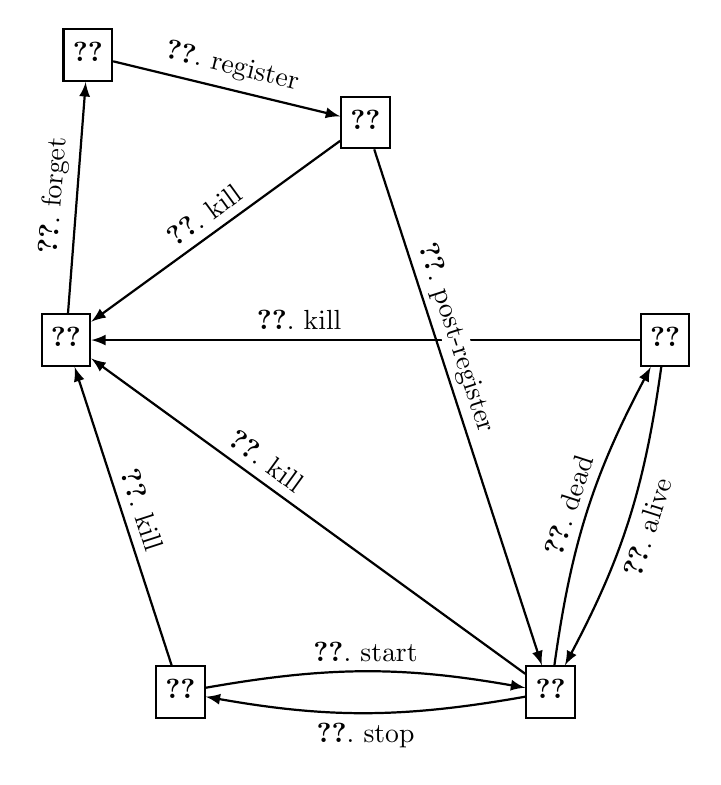
\begin{tikzpicture}
% structure things
% A at 9:30
% B at 12
% ...
% E at 7:30
\foreach \name/\angle/\text in {E/234/E, A/162/A, 
                               B/90/B, C/18/C, D/-54/D}
    \node[circle,draw=white,fill=white,text=white] (\name) at (\angle:4cm) {\text};
\node[circle,draw=white,fill=white,text=white] (F) at (126:6cm) {F};

% Place rectangles for the states
\node[rectangle,minimum height=\baselineskip,draw=black,thick] (unknown)      at (F) {\strut \ref{srvstate:unknown}};
\node[rectangle,minimum height=\baselineskip,draw=black,thick] (assigned)     at (B) {\strut \ref{srvstate:assigned}};
\node[rectangle,minimum height=\baselineskip,draw=black,thick] (notavailable) at (C) {\strut \ref{srvstate:notavailable}};
\node[rectangle,minimum height=\baselineskip,draw=black,thick] (available)    at (D) {\strut \ref{srvstate:available}};
\node[rectangle,minimum height=\baselineskip,draw=black,thick] (shutdown)     at (E) {\strut \ref{srvstate:shutdown}};
\node[rectangle,minimum height=\baselineskip,draw=black,thick] (killed)       at (A) {\strut \ref{srvstate:killed}};

% State transitions
\draw[->,>=latex,thick] (unknown) to node[midway,above,sloped] {\ref{srvtrans:reg}.~register} (assigned);
\draw[->,>=latex,thick] (killed) to node[midway,above,sloped] {\ref{srvtrans:forget}.~forget} (unknown);

\draw[->,>=latex,thick] (notavailable) edge [bend left=10] node[midway,below,sloped] {\ref{srvtrans:alive}.~alive} (available);
\draw[->,>=latex,thick] (available) edge [bend left=10] node[midway,above,sloped] {\ref{srvtrans:dead}.~dead} (notavailable);

\draw[->,>=latex,thick] (available) edge [bend left=10] node[midway,below,sloped] {\ref{srvtrans:stop}.~stop} (shutdown);
\draw[->,>=latex,thick] (shutdown) edge [bend left=10] node[midway,above,sloped] {\ref{srvtrans:start}.~start} (available);

\draw[->,>=latex,thick] (assigned) to node[midway,above,sloped] {\ref{srvtrans:kill}.~kill} (killed);
\draw[->,>=latex,thick] (notavailable) to node[midway,above,sloped,xshift=-24pt] {\ref{srvtrans:kill}.~kill} (killed);
\draw[->,>=latex,thick] (available) to node[midway,above,sloped,xshift=-24pt] {\ref{srvtrans:kill}.~kill} (killed);
\draw[->,>=latex,thick] (shutdown) to node[midway,above,sloped] {\ref{srvtrans:kill}.~kill} (killed);

\draw[->,>=latex,thick] (assigned) -- (available) node[midway,above,sloped,draw=white,fill=white,text=black,rectangle,inner sep=0pt,xshift=-24pt,yshift=2pt] {\ref{srvtrans:postreg}.~post-register};
\end{tikzpicture}
\end{center}
\caption{XXX}
\label{fig:daemon-state-machine}
\end{figure}

\begin{enumerate}[noitemsep]
\item \label{srvtrans:reg} Registration
\item \label{srvtrans:postreg} Post Registration
\item \label{srvtrans:start} Start
\item \label{srvtrans:stop} Stop
\item \label{srvtrans:alive} Alive
\item \label{srvtrans:dead} Dead
\item \label{srvtrans:kill} Kill
\item \label{srvtrans:forget} Forget
\end{enumerate}

\section{Command Reference}
\label{sec:mem:commands}


\part{For Hackers}
\label{part:for-hackers}
\chapter{Writing Client Bindings}
\label{chap:writing-bindigs}


\part{API Reference}
\label{part:api-ref}
\chapter{C API}
\label{chap:api:c}

\section{Client Library}
\label{sec:api:c:client}

The HyperDex Client library, \code{libhyperdex-client} is the de facto way to
access a HyperDex cluster for storing and retrieving data.  All data-store
operations are provided by the this library.

Until release 1.0.rc5, \code{libhyperdex-client} was called
\code{libhyperclient}.  It was changed to be more consistent with the naming of
other HyperDex C libraries.

\subsection{Building the HyperDex C Binding}
\label{sec:api:c:client:build}

The HyperDex C Binding is automatically built and installed via the normal
HyperDex build and install process.  You can ensure that the client is always
built by providing the \code{--enable-client} option to \code{./configure} like
so:

\begin{consolecode}
% ./configure --enable-client
\end{consolecode}

\subsection{Compiling and Linking Your Application}
\label{sec:api:c:client:link}
Unless otherwise noted, all Client operations are defined in the
\code{hyperdex/client.h} include.  You can include this in your own program
with:

\begin{ccode}
#include <hyperdex/client.h>
\end{ccode}

To link against \code{libhyperdex-client}, provide the \code{-lhyperdex-client}
option at link time:

\begin{consolecode}
% cc -o output input.c -I/path/to/hyperdex/include -L/path/to/hyperdex/lib -lhyperdex-client
\end{consolecode}

HyperDex provides support for the automatically determining the compiler and
linker flags for \code{libhyperdex-client}.  First, ensure the \code{pkg-config}
program is installed, and then run:

\begin{consolecode}
% pkg-config --cflags hyperdex-client -I/usr/local/include
% pkg-config --libs hyperdex-client -L/usr/local/lib -lhyperdex-client
\end{consolecode}

The first command outputs the compiler flags necessary to include the
\code{hyperdex/client.h} file, while the second command outputs the flags
necessary for linking against \code{libhyperdex-client}.

To put it all together, you can compile your application with:

\begin{consolecode}
% cc -o output input.c `pkg-config --cflags --libs hyperdex-client`
\end{consolecode}

For more information about \code{pkg-config}, see the
\href{http://people.freedesktop.org/~dbn/pkg-config-guide.html#using}{pkg-config
documentation}.

\subsection{Hello World}
\label{sec:api:c:client:helloworld}

The following is a minimal application that stores the value "Hello World" and
then immediately retrieves the value:

\inputminted{c}{\topdir/api/c/hello-world.c}

You can compile and run this example with:

\begin{consolecode}
% cc -o hello-world hello-world.c `pkg-config --cflags --libs hyperdex-client`
% ./hello-world
put "Hello World!"
get done
got attribute "v" = "Hello World!"
\end{consolecode}

\begin{itemize}
\item Each operation, whether it is a PUT or a GET, is broken down into a
request and a response.  The \code{hyperdex\_client\_put} and
\code{hyperdex\_client\_get} operations each initiate the request.  The
application then calls \code{hyperdex\_client\_loop} to wait for the completion
of the operation.

\item The stored value is passed via \code{struct hyperdex\_client\_attribute}
which specifies both the value of the string "Hello World!" and that this value
is, in fact, a string.  All HyperDex datatypes are passed to HyperDex as
bytestrings via this interface.

\item This code omits error checking, assuming that all operations succeed.  In
the subsequent documentation we'll explore proper error checking, which should
be in place for all non-example code.
\end{itemize}

\subsection{Asynchronous Patterns}
\label{sec:api:c:client:async}

All operations are issued {\em asynchronously}, that is, the operation's start
is decoupled from its completion, and it is up to the application to wait for
its completion.

The C API provides a unified, event-loop-like interface for polling events for
their completion.  An application can issue any number of operations, and poll
for their completion using the \code{hyperdex\_client\_loop} call.  This
provides you with several advantages unavailable in any other distributed
key-value store:

\begin{itemize}
\item Asynchronous events free your application to perform other operations
while waiting for events to complete.

\item Asynchronous events re-use underlying resources, such as TCP connections
to the cluster, across operations.  This enables improved performance and
consumes fewer resources than would be consumed by synchronous clients
generating a similar workload.

\item Operations will be buffered in userspace when they cannot be immediately
sent to a server.  This ensures that applications will never block waiting for
slow servers.
\end{itemize}

Of course, applications do not need to embrace this asynchronous design pattern.
It's always possible to use the library in a synchronous manner by immediately
following every operation with a call to \code{hyperdex\_client\_loop}.

Applications that do embrace this asynchronous design pattern will have a
certain structure.  Specifically:

\begin{itemize}
\item Each operation must eventually be followed by a call to
\code{hyperdex\_client\_loop}.  This is the core of the HyperDex client.  All
work, including flushing userspace buffers, occurs via the call to loop.

\item Pointers used for output from operations must remain valid until
\code{hyperdex\_client\_loop} indicates that the operation has successfully
finished.  Consequently, they must not be aliased to pointers passed to other
operations.
\end{itemize}

Finally, it's important to realize that calling \code{hyperdex\_client\_loop} is
necessary to complete operations.  An operation's outcome is not determined
until the application calls \code{hyperdex\_client\_loop}.  Do not simply issue
\code{hyperdex\_client\_put} operations (or similar) and assume that the
operations complete because there is no guarantee that they will do so.

\subsection{Creating a Client}
\label{sec:api:c:client:create}

A HyperDex client is encapsulated within the incomplete \code{struct
hyperdex\_client} type.  This type is created by the HyperDex client library,
and should only be freed using the provided method.

\begin{ccode}
struct hyperdex_client*
hyperdex_client_create(const char* coordinator, uint16_t port);
\end{ccode}
Create a new client instance.  This call allocates and initializes
local structures.  If allocation or initialization fail, the call will return
NULL and set \code{errno} appropriately.  This call does not establish the
connection to the coordinator; that will be established and maintained
automatically by other calls made with this client instance.

\textbf{Parameters:}
\begin{description}[labelindent=\widthof{{\code{coordinator}}},leftmargin=*,noitemsep,nolistsep,align=right]
\item[\code{coordinator}] A C-string containing IP address or hostname of the
    coordinator.
\item[\code{port}] The port number for the coordinator.
\end{description}

\begin{ccode}
void
hyperdex_client_destroy(struct hyperdex_client* client);
\end{ccode}
Destroy a previously instantiated client, and release all associated
resources.  This call always succeeds.

\textbf{Parameters:}
\begin{description}[labelindent=\widthof{{\code{client}}},leftmargin=*,noitemsep,nolistsep,align=right]
\item[\code{client}] A previously created client instance.
\end{description}

\subsection{Data Structures}
\label{sec:api:c:client:data-structures}

HyperDex natively supports a variety of data structures.  This section describes
the available data structures and their encoding within C.  HyperDex encodes as
a byte string all data structures passed between the application and HyperDex.
This format of this byte string varies according to its type.  In this section,
we'll describe the format of data structures, and provide an API for serializing
to and from the prescribed format.  All APIs discussed in this section are
provided by \code{libhyperdex-client}.

\subsubsection{\code{enum hyperdatatype}}
\label{sec:api:c:client:hyperdatatype}

The \code{enum hyperdatatype} is used to represent the type of a byte string to
HyperDex.  Whenever a structure accepts a byte string as a value, it will
typically accept an \code{enum hyperdatatype} to convey the type of the string.

\paragraph{Primitive Data Types}

Primitive data types are the basic data types of HyperDex.  Applications may use
these primitives as the key and dimensions of hyperspaces within HyperDex.

\begin{description}[noitemsep]
\item[\code{HYPERDATATYPE\_STRING}] A byte string.
\item[\code{HYPERDATATYPE\_INT64}] A 64-bit signed integer.
\item[\code{HYPERDATATYPE\_FLOAT}] A 64-bit floating point value.
\end{description}

\paragraph{Container Data Types}

Container data types contain a collection of primitive data types.  Container
data types cannot be used as the key or dimensions of the hyperspace.

There are three container types available within HyperDex:

\begin{description}
\item[Lists] A list contains elements of one primitive type.  The order of
    elements in a list is preserved, and it's possible for duplicate elements to
    exist.
\item[Sets] A set contains elements of one primitive type.  Each element exists
    in the set at most once.  Although the implementation enforces an order on
    the set for efficiency purposes, set operations are agnostic to the order of
    the included elements.
\item[Maps] A map contains key-value pairs of elements, where the key and value
    may be of different types.  Each key is unique and has an associated value.
    Maps also offer the ability to perform most primitive operations on the
    values within the map.
\end{description}

Each of these containers may be instantiated with a primitive data type as the
contained elements.  In total, HyperDex supports all of the following container
data types:

\begin{description}[noitemsep]
\item[\code{HYPERDATATYPE\_LIST\_STRING}] A list of strings.
\item[\code{HYPERDATATYPE\_LIST\_INT64}] A list of integers.
\item[\code{HYPERDATATYPE\_LIST\_FLOAT}] A list of floats.
\item[\code{HYPERDATATYPE\_SET\_STRING}] A set of strings.
\item[\code{HYPERDATATYPE\_SET\_INT64}] A set of integers.
\item[\code{HYPERDATATYPE\_SET\_FLOAT}] A set of floats.
\item[\code{HYPERDATATYPE\_MAP\_STRING\_STRING}] A map from strings to strings.
\item[\code{HYPERDATATYPE\_MAP\_STRING\_INT64}] A map from strings to integers.
\item[\code{HYPERDATATYPE\_MAP\_STRING\_FLOAT}] A map from strings to floats.
\item[\code{HYPERDATATYPE\_MAP\_INT64\_STRING}] A map from integers to strings.
\item[\code{HYPERDATATYPE\_MAP\_INT64\_INT64}] A map from integers to integers.
\item[\code{HYPERDATATYPE\_MAP\_INT64\_FLOAT}] A map from integers to floats.
\item[\code{HYPERDATATYPE\_MAP\_FLOAT\_STRING}] A map from floats to strings.
\item[\code{HYPERDATATYPE\_MAP\_FLOAT\_INT64}] A map from floats to integers.
\item[\code{HYPERDATATYPE\_MAP\_FLOAT\_FLOAT}] A map from floats to floats.
\end{description}

The following data types are defined as well, and are generally only of interest
to HyperDex developers and those who are writing client bindings:

\begin{description}[noitemsep]
\item[\code{HYPERDATATYPE\_LIST\_GENERIC}] A list whose element type is
    unspecified.
\item[\code{HYPERDATATYPE\_SET\_GENERIC}] A set whose element type is
    unspecified.
\item[\code{HYPERDATATYPE\_MAP\_GENERIC}] A map whose key/value types are
    unspecified.
\item[\code{HYPERDATATYPE\_MAP\_STRING\_KEYONLY}] A map whose key is a string
    and whose value is unspecified.
\item[\code{HYPERDATATYPE\_MAP\_INT64\_KEYONLY}] A map whose key is an integer
    and whose value type is unspecified.
\item[\code{HYPERDATATYPE\_MAP\_FLOAT\_KEYONLY}] A map whose key is a float and
    whose value type is unspecified.
\item[\code{HYPERDATATYPE\_GARBAGE}] A reserved constant never used within
    HyperDex.
\end{description}

\subsubsection{Bytestring Format}
\label{sec:api:c:client:format}

The format of the data structures is defined to be the same on all platforms.

For each format, Python-like psuedocode is provided that shows example
encodings.

\paragraph{string format}

A string is an 8-bit byte string.  HyperDex is agnostic to the contents of the
string, and it may contain any bytes, including \code{\\x00}.  By convention,
the trailing \code{NULL} should be omitted for C-strings to ensure
interoperability across languages.  For example:

\begin{pythoncode}
>>> encode_string('Hello\x00World!')
b'Hello\x00World!'
\end{pythoncode}

\paragraph{int format}

Integers are encoded as signed 8-byte little-endian integers.  For example:

\begin{pythoncode}
>>> encode_int(1)
b'\x01\x00\x00\x00\x00\x00\x00\x00'
>>> encode_int(-1)
b'\xff\xff\xff\xff\xff\xff\xff\xff'
>>> encode_int(0xdeadbeef)
b'\xef\xbe\xad\xde\x00\x00\x00\x00'
\end{pythoncode}

\paragraph{float format}

Floats are encoded as IEEE 754 binary64 values in little-endian format.  For
example:

\begin{pythoncode}
>>> encode_double(0)
b'\x00\x00\x00\x00\x00\x00\x00\x00'
>>> encode_double(3.1415)
b'o\x12\x83\xc0\xca!\t@'
\end{pythoncode}

\paragraph{list(string) format}

Lists of strings are encoded by concatenating the encoding of each string,
prefixed by an unsigned 4-byte little endian integer indicating the length of
the string.  For example:

\begin{pythoncode}
>>> encode_list_string([])
b''
>>> encode_list_string(['hello', 'world'])
b'\x05\x00\x00\x00hello\x05\x00\x00\x00world'
\end{pythoncode}

\paragraph{list(int) format}

Lists of integers are encoded by concatenating the encoded form of each integer.
For example:

\begin{pythoncode}
>>> encode_list_int([])
b''
>>> encode_list_int([1, -1, 0xdeadbeef])
b'\x01\x00\x00\x00\x00\x00\x00\x00' \
b'\xff\xff\xff\xff\xff\xff\xff\xff' \
b'\xef\xbe\xad\xde\x00\x00\x00\x00'
\end{pythoncode}

\paragraph{list(floats) format}

Lists of floats are encoded by concatenating the encoded form of each float.
For example:

\begin{pythoncode}
>>> encode_list_float([])
b''
>>> encode_list_float([0, 3.1415])
b'\x00\x00\x00\x00\x00\x00\x00\x00' \
b'o\x12\x83\xc0\xca!\t@'
\end{pythoncode}

\paragraph{set(string) format}

Sets of strings are encoded by concatenating the encoding of each string in
sorted order, where each string is prefixed by an unsigned 4-byte little endian
integer indicating the length of the string.  For example:

\begin{pythoncode}
>>> encode_set_string([])
b''
>>> encode_set_string(['world', 'hello'])
b'\x05\x00\x00\x00hello\x05\x00\x00\x00world'
\end{pythoncode}

\paragraph{set(int) format}

Sets of integers are encoded by concatenating the encoded form of each integer
in sorted order.  For example:

\begin{pythoncode}
>>> encode_set_int([])
b''
>>> encode_set_int([1, -1, 0xdeadbeef])
b'\xff\xff\xff\xff\xff\xff\xff\xff' \
b'\x01\x00\x00\x00\x00\x00\x00\x00' \
b'\xef\xbe\xad\xde\x00\x00\x00\x00'
\end{pythoncode}

\paragraph{set(float) format}

Sets of floats are encoded by concatenating the encoded form of each float in
sorted order.  For example:

\begin{pythoncode}
>>> encode_set_float([])
b''
>>> encode_set_float([3.1415, 0])
b'\x00\x00\x00\x00\x00\x00\x00\x00' \
b'o\x12\x83\xc0\xca!\t@'
\end{pythoncode}

\paragraph{map(string, string) format}

Maps from strings to strings are formed by encoding the individual elements,
each prefixed by an unsigned 4-byte little endian integer indicating their
length.  The pairs of elements are stored in sorted order according to the first
element of the pair (the map's key).  For example:

\begin{pythoncode}
>>> encode_map_string_string({})
b''
>>> encode_map_string_string({'hello': 'world',
...                           'map key': 'map val',
...                           'map', 'encoding'})
b'\x05\x00\x00\x00hello\x05\x00\x00\x00world' \
b'\x03\x00\x00\x00map\x08\x00\x00\x00encoding' \
b'\x07\x00\x00\x00map key\x07\x00\x00\x00map val'
\end{pythoncode}

\paragraph{map(string, int) format}

Maps from strings to ints are formed by encoding the individual elements, where
keys are prefixed by an unsigned 4-byte little endian integer indicating their
length.  The pairs of elements are stored in sorted order according to the first
element of the pair (the map's key).  For example:

\begin{pythoncode}
>>> encode_map_string_int({})
b''
>>> encode_map_string_int({'world': -1,
...                        'hello': 1})
b'\x05\x00\x00\x00hello\x01\x00\x00\x00\x00\x00\x00\x00' \
b'\x05\x00\x00\x00world\xff\xff\xff\xff\xff\xff\xff\xff'
\end{pythoncode}

\paragraph{map(string, float) format}

Maps from strings to ints are formed by encoding the individual elements, where
keys are prefixed by an unsigned 4-byte little endian integer indicating their
length.  The pairs of elements are stored in sorted order according to the first
element of the pair (the map's key).  For example:

\begin{pythoncode}
>>> encode_map_string_float({})
b''
>>> encode_map_string_float({'zero': 0,
...                          'pi': 3.1415})
b'\x02\x00\x00\x00pio\x12\x83\xc0\xca!\t@' \
b'\x04\x00\x00\x00zero\x00\x00\x00\x00\x00\x00\x00\x00'
\end{pythoncode}

\paragraph{map(int, string) format}

Maps from ints to strings are formed by encoding the individual elements, where
values are prefixed by an unsigned 4-byte little endian integer indicating their
length.  The pairs of elements are stored in sorted order according to the first
element of the pair (the map's key).  For example:

\begin{pythoncode}
>>> encode_map_int_string({})
b''
>>> encode_map_int_string({1: 'hello',
...                        -1: 'world'})
b'\xff\xff\xff\xff\xff\xff\xff\xff\x05\x00\x00\x00world' \
b'\x01\x00\x00\x00\x00\x00\x00\x00\x05\x00\x00\x00hello'
\end{pythoncode}

\paragraph{map(int, int) format}

Maps from ints to ints are formed by encoding the individual elements.  The
pairs of elements are stored in sorted order according to the first element of
the pair (the map's key).  For example:

\begin{pythoncode}
>>> encode_map_int_int({})
b''
>>> encode_map_int_int({1: 0xdeadbeef,
...                     -1: 0x1eaff00d})
b'\xff\xff\xff\xff\xff\xff\xff\xff\x0d\xf0\xaf\x1e\x00\x00\x00\x00' \
b'\x01\x00\x00\x00\x00\x00\x00\x00\xef\xbe\xad\xde\x00\x00\x00\x00'
\end{pythoncode}

\paragraph{map(int, float) format}

Maps from ints to floats are formed by encoding the individual elements.  The
pairs of elements are stored in sorted order according to the first element of
the pair (the map's key).  For example:

\begin{pythoncode}
>>> encode_map_int_float({})
b''
>>> encode_map_int_float({1: 0,
...                       -1: 3.1415})
b'\xff\xff\xff\xff\xff\xff\xff\xffo\x12\x83\xc0\xca!\t@' \
b'\x01\x00\x00\x00\x00\x00\x00\x00\x00\x00\x00\x00\x00\x00\x00\x00'
\end{pythoncode}

\paragraph{map(float, string) format}

Maps from floats to strings are formed by encoding the individual elements,
where values are prefixed by an unsigned 4-byte little endian integer indicating
their length.  The pairs of elements are stored in sorted order according to the
first element of the pair (the map's key).  For example:

\begin{pythoncode}
>>> encode_map_float_string({})
b''
>>> encode_map_float_string({0: 'hello',
...                          3.1415: 'world'})
b'\x00\x00\x00\x00\x00\x00\x00\x00\x05\x00\x00\x00hello' \
b'o\x12\x83\xc0\xca!\t@\x05\x00\x00\x00world'
\end{pythoncode}

\paragraph{map(float, int) format}

Maps from floats to ints are formed by encoding the individual elements.  The
pairs of elements are stored in sorted order according to the first element of
the pair (the map's key).  For example:

\begin{pythoncode}
>>> encode_map_float_int({})
b''
>>> encode_map_float_int({0: 1,
...                       3.1415: -1})
b'\x00\x00\x00\x00\x00\x00\x00\x00\x01\x00\x00\x00\x00\x00\x00\x00' \
b'o\x12\x83\xc0\xca!\t@\xff\xff\xff\xff\xff\xff\xff\xff'
\end{pythoncode}

\paragraph{map(float, float) format}

Maps from floats to floats are formed by encoding the individual elements.  The
pairs of elements are stored in sorted order according to the first element of
the pair (the map's key).  For example:

\begin{pythoncode}
>>> encode_map_float_float({})
b''
>>> encode_map_float_float({0: 1,
...                         3.1415: -1})
b'\x00\x00\x00\x00\x00\x00\x00\x00\x00\x00\x00\x00\x00\x00\xf0?' \
b'o\x12\x83\xc0\xca!\t@\x00\x00\x00\x00\x00\x00\xf0\xbf'
\end{pythoncode}

\subsubsection{Serialization API}
\label{sec:api:c:client:serialize}

The serialization API supports serialization of all datatypes supported by
HyperDex.  Of course, feel free to manually encode data structures, especially
where doing so can make use of efficient stack-allocated data structures.

\paragraph{struct hyperdex\_ds\_arena}

The packing routines described below may occasionally have to allocate memory
into which the encoded forms of the datatypes are copied.  To free the
programmer from the burden of having to manually allocate and free each of these
pieces of memory, the data structures API allocates all memory via an instance
of \code{struct hyperdex\_ds\_arena}.  Via a single call to
\code{hyperdex\_ds\_arena\_destroy}, all memory allocated via the arena is
free'd.

\code{struct hyperdex\_ds\_arena} is intentionally defined as an incomplete type
because its internals are subject to change.  To create an arena, call
\code{hyperdex\_ds\_arena\_create}.  The arena should subsequently be destroyed
via \code{hyperdex\_ds\_arena\_destroy}.

\begin{ccode}
struct hyperdex_ds_arena* hyperdex_ds_arena_create();
\end{ccode}
Create a new arena for alocating memory.  On success, this function
returns a non-null pointer for the new arena.  On failure, the function returns
\code{NULL}, indicating that memory allocation failed.  It is the caller's
responsibility to pass this function to \code{hyperdex\_ds\_arena\_destroy} when
finished.

\begin{ccode}
void hyperdex_ds_arena_destroy(struct hyperdex_ds_arena* arena);
\end{ccode}
Free all memory associated with \code{arena}.  This function always
succeeds.

\paragraph{serialize string}

No serialization is necessary for string data types.  For convenience, the
serialization API provides a copy function that copies a string into
arena-allocated memory.

\begin{ccode}
int hyperdex_ds_copy_string(struct hyperdex_ds_arena* arena, const char* str,
                            size_t str_sz, enum hyperdex_ds_returncode* status,
                            const char** value, size_t* value_sz);
\end{ccode}
Copy the string \code{str}/\code{str\_sz} into memory allocated via
\code{arena} and return the copy via \code{value} and \code{value\_sz}.  This
function will fail and return -1 if there is insufficient memory available for
copying the string.  All pointers returned by this function remain valid until
\code{arena} is destroyed.  The client should not attempt to free the returned
copy.

\paragraph{serialize int}

\begin{ccode}
void hyperdex_ds_pack_int(int64_t num, char* value);
\end{ccode}
Packs \code{num} into the bytes pointed to by \code{buf}.  This
function always succeeds.  It is the caller's responsibility to ensure that
\code{buf} points to at least \unit{8}{\byte}.

\begin{ccode}
int hyperdex_ds_copy_int(struct hyperdex_ds_arena* arena, int64_t num,
                         enum hyperdex_ds_returncode* status,
                         const char** value, size_t* value_sz);
\end{ccode}
Encode \code{num} into memory allocated via \code{arena} and return
the value via \code{value} and \code{value\_sz}.  This function will fail and
return -1 if there is insufficient memory available for encoding the nubmer.
All pointers returned by this function remain valid until \code{arena} is
destroyed.  The client should not attempt to free the returned copy.

\paragraph{serialize float}

\begin{ccode}
void hyperdex_ds_pack_float(double num, char* value);
\end{ccode}
Pack \code{num} into the bytes pointed to by \code{buf}.  This
function always succeeds.  It is the caller's responsibility to ensure that
\code{buf} points to at least \unit{8}{\byte}.

\begin{ccode}
int hyperdex_ds_copy_float(struct hyperdex_ds_arena* arena, double num,
                           enum hyperdex_ds_returncode* status,
                           const char** value, size_t* value_sz);
\end{ccode}
Encode \code{num} into memory allocated via \code{arena} and return
the value via \code{value} and \code{value\_sz}.  This function will fail and
return -1 if there is insufficient memory available for encoding the nubmer.
All pointers returned by this function remain valid until \code{arena} is
destroyed.  The client should not attempt to free the returned copy.

\paragraph{serialize lists}

The below functions incrementally build lists, performing all relevant error
checking to ensure that the resuling HyperDex list is well-formed.  The first
element appended to the list implicitly determines the type of the list.  All
subsequent calls that push elements of a different type will fail.

\begin{ccode}
struct hyperdex_ds_list* hyperdex_ds_allocate_list(struct hyperdex_ds_arena* arena);
\end{ccode}
Create a new dynamic list.  This function will fail and return
\code{NULL} should memory allocation fail.

\begin{ccode}
int hyperdex_ds_list_insert_string(struct hyperdex_ds_list* list,
                                   const char* str, size_t str_sz,
                                   enum hyperdex_ds_returncode* status);
\end{ccode}
Append the string \code{str}/\code{str\_sz} to \code{list}.  This
function will fail and return -1 if memory allocation fails, or the list is not
a list of strings.

\begin{ccode}
int hyperdex_ds_list_insert_int(struct hyperdex_ds_list* list, int64_t num,
                                enum hyperdex_ds_returncode* status);
\end{ccode}
Append the integer \code{num} to \code{list}.  This function will fail
and return -1 if memory allocation fails, or the list is not a list of integers.

\begin{ccode}
int hyperdex_ds_list_insert_float(struct hyperdex_ds_list* list, double num,
                                  enum hyperdex_ds_returncode* status);
\end{ccode}
Append the float \code{num} to \code{list}.  This function will fail
and return -1 if memory allocation fails or the list is not a list of floats.

\begin{ccode}
int hyperdex_ds_list_finalize(struct hyperdex_ds_list*,
                              enum hyperdex_ds_returncode* status,
                              const char** value, size_t* value_sz,
                              enum hyperdatatype* datatype);
\end{ccode}
Finalize the list by writing its elements into a bytestring.  This
function returns the bytestring and the list type.  It will fail and return -1
if memory allocation fails.

\paragraph{serialize sets}

The below functions incrementally build sets, performing all relevant error
checking to ensure that the resuling HyperDex set is well-formed.  The first
element inserted into the set implicitly determines the type of the set.  All
subsequent calls that insert elements of different types will fail.

\begin{ccode}
struct hyperdex_ds_set* hyperdex_ds_allocate_set(struct hyperdex_ds_arena* arena);
\end{ccode}
Create a new dynamic set.  This function will fail and return
\code{NULL} should memory allocation fail.

\begin{ccode}
int hyperdex_ds_set_insert_string(struct hyperdex_ds_set* set,
                                  const char* str, size_t str_sz,
                                  enum hyperdex_ds_returncode* status);
\end{ccode}
Insert the string \code{str}/\code{str\_sz} into \code{set}.  This
function will fail and return -1 if memory allocation fails, or the set is not a
set of strings.

\begin{ccode}
int hyperdex_ds_set_insert_int(struct hyperdex_ds_set* set, int64_t num,
                               enum hyperdex_ds_returncode* status);
\end{ccode}
Insert the integer \code{num} into \code{set}.  This function will
fail and return -1 if memory allocation fails, or the set is not a set of
integers.

\begin{ccode}
int hyperdex_ds_set_insert_float(struct hyperdex_ds_set* set, double num,
                                 enum hyperdex_ds_returncode* status);
\end{ccode}
Insert the float \code{num} into \code{set}.  This function will fail
and return -1 if memory allocation fails, or the set is not a set of floats.

\begin{ccode}
int hyperdex_ds_set_finalize(struct hyperdex_ds_set*,
                             enum hyperdex_ds_returncode* status,
                             const char** value, size_t* value_sz,
                             enum hyperdatatype* datatype);
\end{ccode}
Finalize the set by writing its elements into a bytestring.  This
function returns the bytestring and the set type.  It will fail and return -1 if
memory allocation fails.

\paragraph{serialize maps}

The below functions incrementally build maps, performing all relevant error
checking to ensure that the resuling HyperDex map is well-formed.  The first
key/value-pair inserted into the map implicitly determines the type of the map.  All
subsequent calls that insert elements of different types will fail.

The map is built by alternating calls to the key/value functions described
below, starting with a key-based function.  This keeps the number of cases
linear in the number of primitive types a map may contain, rather than appending
key-value pairs directly (which would require a quadratic number of calls).

\begin{ccode}
struct hyperdex_ds_map* hyperdex_ds_allocate_map(struct hyperdex_ds_arena* arena);
\end{ccode}
Create a new dynamic map.  This function will fail and return
\code{NULL} should memory allocation fail.

\begin{ccode}
int hyperdex_ds_map_insert_key_string(struct hyperdex_ds_map* map,
                                      const char* str, size_t str_sz,
                                      enum hyperdex_ds_returncode* status);
\end{ccode}
Set the key of the next pair to be inserted into \code{map} to the
string specified by \code{str} and \code{str\_sz}.  This function will fail and
return -1 if memory allocation fails, or the map does not use strings for keys.

\begin{ccode}
int hyperdex_ds_map_insert_val_string(struct hyperdex_ds_map* map,
                                      const char* str, size_t str_sz,
                                      enum hyperdex_ds_returncode* status);
\end{ccode}
Set the value of the next pair to be inserted into \code{map} to the
string specified by \code{str} and \code{str\_sz}, and insert the pair.  This
function will fail and return -1 if memory allocation fails, or the map does not
use strings for values.

\begin{ccode}
int hyperdex_ds_map_insert_key_int(struct hyperdex_ds_map* map,
                                   int64_t num,
                                   enum hyperdex_ds_returncode* status);
\end{ccode}
Set the key of the next pair to be inserted into \code{map} to the
integer specified by \code{num}.  This function will fail and return -1 if
memory allocation fails, or the map does not nuse integers for keys.

\begin{ccode}
int hyperdex_ds_map_insert_val_int(struct hyperdex_ds_map* map,
                                   int64_t num,
                                   enum hyperdex_ds_returncode* status);
\end{ccode}
Set the value of the next pair to be inserted into \code{map} to the
integer specified by \code{num}, and insert the pair.  This function will fail
and return -1 if memory allocation fails, or the map does not use integers for
values.

\begin{ccode}
int hyperdex_ds_map_insert_key_float(struct hyperdex_ds_map* map,
                                     double num,
                                     enum hyperdex_ds_returncode* status);
\end{ccode}
Set the key of the next pair to be inserted into \code{map} to the
float specified by \code{num}.  This function will fail and return -1 if memory
allocation fails, or the map does not use floats for keys.

\begin{ccode}
int hyperdex_ds_map_insert_val_float(struct hyperdex_ds_map* map,
                                     double num,
                                     enum hyperdex_ds_returncode* status);
\end{ccode}
Set the value of the next pair to be inserted into \code{map} to the
float specified by \code{num}.  This function will fail and return -1 if memory
allocation fails, or the map does not use floats for values.

\begin{ccode}
int hyperdex_ds_map_finalize(struct hyperdex_ds_map*,
                             enum hyperdex_ds_returncode* status,
                             const char** value, size_t* value_sz,
                             enum hyperdatatype* datatype);
\end{ccode}
Finalize the map by writing its key/value-pairs  into a bytestring.
This function returns the bytestring and the map type.  It will fail and return
-1 if memory allocation fails, or an uneven number of key/value calls were made.

\subsubsection{Deserialization API}
\label{sec:api:c:client:deserialize}

The deserialization API provides routines to unpack ints and floats, and iterate
the elements in lists, sets, and maps.  Iterators return elements one-by-one
with a minimal amount of copying and allocation.  All iterators are used in the
same pattern.  For example, to iterate a list of integers:

\inputminted{c}{\topdir/api/c/iterate.c}

Compile and run this example with:

\begin{consolecode}
$ cc -o iterate iterate.c `pkg-config --cflags --libs hyperdex-client`
$ ./iterate
1
-1
3735928559
\end{consolecode}

The function \code{hyperdex\_ds\_iterator\_init} sets up the iterator.  Each
container data type has a specialized iteration function.  All iterators share
the same initialization function.

\begin{ccode}
void hyperdex_ds_iterator_init(struct hyperdex_ds_iterator* iter,
                               enum hyperdatatype datatype,
                               const char* value,
                               size_t value_sz);
\end{ccode}
Initialize an iterator for the given data type/value.  This function
always succeeds.

\paragraph{deserialize string}

No deserialization is necessary for string data types.

\paragraph{deserialize int}

\begin{ccode}
int hyperdex_ds_unpack_int(const char* buf, size_t buf_sz, int64_t* num);
\end{ccode}
Unpack \code{num} from \code{buf}/\code{buf\_sz}.  This function will
fail and return -1 if \code{buf\_sz} is not exactly \unit{8}{\byte}.

\paragraph{deserialize float}

\begin{ccode}
int hyperdex_ds_unpack_float(const char* buf, size_t buf_sz, double* num);
\end{ccode}
Unpack \code{num} from \code{buf}/\code{buf\_sz}.  This function will
fail and return -1 if \code{buf\_sz} is not exactly \unit{8}{\byte}.

\paragraph{deserialize lists}

\begin{ccode}
int hyperdex_ds_iterate_list_string_next(struct hyperdex_ds_iterator* iter,
                                         const char** str, size_t* str_sz);
\end{ccode}
Return the next string element in the list.  This function will return
1 if an element is returned, 0 if there are no elements to return, and -1 if the
list of strings is malformed.  The falue stored in \code{*str} is a pointer into
the list of strings and should not be free'd by the application.

\begin{ccode}
int hyperdex_ds_iterate_list_int_next(struct hyperdex_ds_iterator* iter, int64_t* num);
\end{ccode}
Return the next integer element in the list.  This function will
return 1 if an element is returned, 0 if there are no elements to return, and -1
if the list of integers is malformed.

\begin{ccode}
int hyperdex_ds_iterate_list_float_next(struct hyperdex_ds_iterator* iter, double* num);
\end{ccode}
Return the next float element in the list.  This function will return
1 if an element is returned, 0 if there are no elements to return, and -1 if the
list of floats is malformed.

\paragraph{deserialize sets}

\begin{ccode}
int hyperdex_ds_iterate_set_string_next(struct hyperdex_ds_iterator* iter,
                                        const char** str, size_t* str_sz);
\end{ccode}
Return the next string element in the set.  This function will return
1 if an element is returned, 0 if there are no elements to return, and -1 if the
set of strings is malformed.  The value stored in \code{*str} is a pointer into
the set of strings and should not be free'd by the application.

\begin{ccode}
int hyperdex_ds_iterate_set_int_next(struct hyperdex_ds_iterator* iter, int64_t* num);
\end{ccode}
Return the next integer element in the set.  This function will return
1 if an element is returned, 0 if there are no elements to return, and -1 if the
set of ints is malformed.

\begin{ccode}
int hyperdex_ds_iterate_set_float_next(struct hyperdex_ds_iterator* iter, double* num);
\end{ccode}
Return the next float element in the set.  This function will return 1
if an element is returned, 0 if there are no elements to return, and -1 if the
set of ints is malformed.

\paragraph{deserialize maps}

\begin{ccode}
int hyperdex_ds_iterate_map_string_string_next(struct hyperdex_ds_iterator* iter,
                                               const char** key, size_t* key_sz,
                                               const char** val, size_t* val_sz);
\end{ccode}
Return the next pair of (string, string) in the map.  This function
will return 1 if an element is returned, 0 if there are no elements to return,
and -1 if the map is malformed.  The values stored in \code{*key} and
\code{*val} are pointers into the map and should not be free'd by the
application.

\begin{ccode}
int hyperdex_ds_iterate_map_string_int_next(struct hyperdex_ds_iterator* iter,
                                            const char** key, size_t* key_sz,
                                            int64_t* val);
\end{ccode}
Return the next pair of (string, int) in the map.  This function will
return 1 if an element is returned, 0 if there are no elements to return, and -1
if the map is malformed.  The value stored in \code{*key} is a pointer into the
map and should not be free'd by the application.

\begin{ccode}
int hyperdex_ds_iterate_map_string_float_next(struct hyperdex_ds_iterator* iter,
                                              const char** key, size_t* key_sz,
                                              double* val);
\end{ccode}
Return the next pair of (string, float) in the map.  This function
will return 1 if an element is returned, 0 if there are no elements to return,
and -1 if the map is malformed.  The value stored in \code{*key} is a pointer
into the map and should not be free'd by the application.

\begin{ccode}
int hyperdex_ds_iterate_map_int_string_next(struct hyperdex_ds_iterator* iter,
                                            int64_t* key,
                                            const char** val, size_t* val_sz);
\end{ccode}
Return the next pair of (int, string) in the map.  This function will
return 1 if an element is returned, 0 if there are no elements to return, and -1
if the map is malformed.  The value stored in \code{*val} is a pointer into the
map and should not be free'd by the application.

\begin{ccode}
int hyperdex_ds_iterate_map_int_int_next(struct hyperdex_ds_iterator* iter,
                                         int64_t* key, int64_t* val);
\end{ccode}
Return the next pair of (int, int) in the map.  This function will
return 1 if an element is returned, 0 if there are no elements to return, and -1
if the map is malformed.

\begin{ccode}
int hyperdex_ds_iterate_map_int_float_next(struct hyperdex_ds_iterator* iter,
                                           int64_t* key, double* val);
\end{ccode}
Return the next pair of (int, float) in the map.  This function will
return 1 if an element is returned, 0 if there are no elements to return, and -1
if the map is malformed.

\begin{ccode}
int hyperdex_ds_iterate_map_float_string_next(struct hyperdex_ds_iterator* iter,
                                              double* key,
                                              const char** val, size_t* val_sz);
\end{ccode}
Return the next pair of (float, string) in the map.  This function
will return 1 if an element is returned, 0 if there are no elements to return,
and -1 if the map is malformed.  The value stored in \code{*val} is a pointer
into the map and should not be free'd by the application.

\begin{ccode}
int hyperdex_ds_iterate_map_float_int_next(struct hyperdex_ds_iterator* iter,
                                           double* key, int64_t* val);
\end{ccode}
Return the next pair of (float, int) in the map.  This function will
return 1 if an element is returned, 0 if there are no elements to return, and -1
if the map is malformed.

\begin{ccode}
int hyperdex_ds_iterate_map_float_float_next(struct hyperdex_ds_iterator* iter,
                                             double* key, double* val);
\end{ccode}
Return the next pair of (float, float) in the map.  This function will
return 1 if an element is returned, 0 if there are no elements to return, and -1
if the map is malformed.

\subsubsection{Memory Management Utilties}
\label{sec:api:c:client:memory}

The data structures API provides utility functions for allocating structures
from the arena, obviating the need to free them individually.

\begin{ccode}
struct hyperdex_client_attribute*
hyperdex_ds_allocate_attribute(struct hyperdex_ds_arena* arena, size_t sz);
\end{ccode}
Allocate an array of \code{struct hyperdex\_client\_attribute}.  On
success, this function returns a non-null pointer containing \code{sz} elements.
On failure, the function returns \code{NULL}, indicating that memory allocation
failed.  The memory will remain valid until the arena is destroyed and should
not be free'd independently by the application.

\begin{ccode}
struct hyperdex_client_attribute_check*
hyperdex_ds_allocate_attribute_check(struct hyperdex_ds_arena* arena, size_t sz);
\end{ccode}
Allocate an array of \code{struct hyperdex\_client\_attribute\_check}.
On success, this function returns a non-null pointer containing \code{sz}
elements.  On failure, the function returns \code{NULL}, indicating that memory
allocation failed.  The memory will remain valid until the arena is destroyed
and should not be free'd independently by the application.

\begin{ccode}
struct hyperdex_client_map_attribute*
hyperdex_ds_allocate_map_attribute(struct hyperdex_ds_arena* arena, size_t sz);
\end{ccode}
Allocate an array of \code{struct hyperdex\_client\_map\_attribute}.
On success, this function returns a non-null pointer containing \code{sz}
elements.  On failure, the function returns \code{NULL}, indicating that memory
allocation failed.  The memory will remain valid until the arena is destroyed
and should not be free'd independently by the application.

\subsection{Attributes}
\label{sec:api:c:client:attributes}

In HyperDex, {\em attributes} specified named values that comprise an object.
For instance, in Chapter~\nameref{chap:quick-start}, the phonebook space has
attributes ``username'', ``first'', ``last'', and ``phone''.  The C API
represents such attributes using \code{struct hyperdex\_client\_attribute}.  The
C definition of this struct is:

\begin{ccode}
struct hyperdex_client_attribute
{
    const char* attr; /* NULL-terminated */
    const char* value;
    size_t value_sz;
    enum hyperdatatype datatype;
};
\end{ccode}

This struct specifies the name, value, and data type of the attribute.  The
\code{attr} field is a NULL-terminated C-string that names the attribute
affected by the value.  The \code{value} and \code{value\_sz} fields contain a
properly formatted byte string and its size.  The \code{datatype} field
indicates the encoding of the byte string.

The interpretation of an attribute is dependent upon the operation being
performed.  In the case of \code{hyperdex\_client\_put}, the attributes directly
convey the values to be stored; \code{hyperdex\_client\_get} returns the
stored attributes.  Other operations, such as
\code{hyperdex\_client\_string\_prepend} interpret the attribute as an argument
to the operation.  In the case of prepend, the attribute specifies the value to
be prepended.

\subsection{Map Attributes}
\label{sec:api:c:client:map-attributes}

Some HyperDex operations affect key-value pairs contained within maps.  These
operations use \code{struct hyperdex\_client\_map\_attribute} to specify the
name of the attribute affected, the key within the map, and the value associated
with that key.  The C definition of this struct is:

\begin{ccode}
struct hyperdex_client_map_attribute
{
    const char* attr; /* NULL-terminated */
    const char* map_key;
    size_t map_key_sz;
    enum hyperdatatype map_key_datatype;
    const char* value;
    size_t value_sz;
    enum hyperdatatype value_datatype;
};
\end{ccode}

The struct specifies the name, key, and value of to be used for the operation.
The \code{map\_key\_*} and \code{value\_*} fields specify, respectively, the key
and value of the element within the map.  The relative fields are specified as
byte strings with associated data types.  The \code{attr} field specifies the
name of the map.

\subsection{Predicates}
\label{sec:api:c:client:predicates}

In HyperDex, a {\em predicate} is an expression about an attribute that is true
or false.  Predicates are specified to HyperDex using \code{struct
hyperdex\_client\_attribute\_check} which is defined as:

\begin{ccode}
struct hyperdex_client_attribute_check
{
    const char* attr; /* NULL-terminated */
    const char* value;
    size_t value_sz;
    enum hyperdatatype datatype;
    enum hyperpredicate predicate;
};
\end{ccode}

Note that this struct closely resembes \code{struct
hyperdex\_client\_attribute}, with the addition of a field named
\code{predicate}.  This field is an enum with the following values:

\begin{description}
\item[\code{HYPERPREDICATE\_FAIL}] Always fail.
\item[\code{HYPERPREDICATE\_EQUALS}] Check that the existing value is equal to
    the one specified by \code{value}/\code{value\_sz}.
\item[\code{HYPERPREDICATE\_LESS\_EQUAL}] Check that the existing value is less
    than or equal to the one specified by \code{value}/\code{value\_sz}.
\item[\code{HYPERPREDICATE\_GREATER\_EQUAL}] Check that the existing value is
    greater than or equal to the one specified by \code{value}/\code{value\_sz}.
\item[\code{HYPERPREDICATE\_REGEX}] Check that the existing value matches the
    regular expression stored in as a string in \code{value}/\code{value\_sz}.
\item[\code{HYPERPREDICATE\_LENGTH\_EQUALS}] Check that the existing container
    or string has a length equal to the integer stored in
    \code{value}/\code{value\_sz}.
\item[\code{HYPERPREDICATE\_LENGTH\_LESS\_EQUAL}] Check that the existing
    container or string has a length less than or equal to the integer stored in
    \code{value}/\code{value\_sz}.
\item[\code{HYPERPREDICATE\_LENGTH\_GREATER\_EQUAL}] Check that the existing
    container or string has a length greater than or equal to the integer stored
    in \code{value}/\code{value\_sz}.
\item[\code{HYPERPREDICATE\_CONTAINS}] Check that the container contains an
    element matching \code{value}/\code{value\_sz}.
\end{description}

\subsection{Error Handling}
\label{sec:api:c:client:error-handling}

Every call in the client provides a means for reporting failure.  After each
call, your application should check for the error and react appropriately.
Depending upon the error, your application may retry the request, or may need to
take more drastic action.

Errors are typically reported via \code{enum hyperdex\_client\_returncode}
defined in \code{hyperdex/client.h}.  Values for this enum fall into three
categories:  values returned during normal operation, values returned to
indicate anticipated errors, and values that should never be returned in
practice.

The common-case returncodes are:

\begin{description}
\item[\code{HYPERDEX\_CLIENT\_SUCCESS}]  The operation was successful and no
    errors occurred.
\item[\code{HYPERDEX\_CLIENT\_NOTFOUND}]  The operation finished because the
    requested object was not found.
\item[\code{HYPERDEX\_CLIENT\_SEARCHDONE}]  An operation that potentially
    returns multiple objects.  For instance, a search has
    finished and will no longer be returned via loop.
\item[\code{HYPERDEX\_CLIENT\_CMPFAIL}]  The predicate specified as part of a
    conditional operation was not true.
\item[\code{HYPERDEX\_CLIENT\_READONLY}] The cluster is in read-only mode and
    not accepting write operations.
\end{description}

The following errors stem from environmental problems or problems with the
application's usage of HyperDex.  These errors are generally easy to remedy and
are anticipated by the client library.

\begin{description}
\item[\code{HYPERDEX\_CLIENT\_UNKNOWNSPACE}] The specified space does not exist.
    Ensure that a space exists before trying to manipulate its data.
\item[\code{HYPERDEX\_CLIENT\_COORDFAIL}] The connection to the coordinator has
    failed.  The application should back off before retrying.

    Note that the connection to the coordinator is not a simple TCP connection,
    and is redundant if the coordinator consists of multiple servers.  This
    error indicates to the application that the redundancy has failed and that
    the application should back-off.
\item[\code{HYPERDEX\_CLIENT\_SERVERERROR}] A server returned a nonsensical
    result to the client library.  Generally retrying the request should be
    sufficient to overcome the problem.
\item[\code{HYPERDEX\_CLIENT\_POLLFAILED}] The poll system call failed in an
    unexpected manner.  Typically, this means that the application using the
    HyperDex library has mismanaged its file descriptors and improperly altered
    descriptors in use by the HyperDex library.

    This generally indicates that there is a bug in the HyperDex client library,
    the application using the library, or both.
\item[\code{HYPERDEX\_CLIENT\_OVERFLOW}] An integer operation failed to complete
    because it would have resulted in signed overflow.
\item[\code{HYPERDEX\_CLIENT\_RECONFIGURE}] The server responsible for managing
    the operation failed while the operation was in-flight.
\item[\code{HYPERDEX\_CLIENT\_TIMEOUT}] The \code{hyperdex\_client\_loop}
    operation exceeded its timeout without completing an outstanding operation.
    This does not affect the status of any outstanding operation.
\item[\code{HYPERDEX\_CLIENT\_UNKNOWNATTR}] The operation references an
    attribute that is not part of the space.  Make sure to use attributes within
    the space's schema.
\item[\code{HYPERDEX\_CLIENT\_DUPEATTR}] The operation references an attribute
    multiple times in a way that is not permitted.
\item[\code{HYPERDEX\_CLIENT\_NONEPENDING}] The \code{hyperdex\_client\_loop}
    call was made, but no operations were outstanding.  This generally indicates
    that the loop call was called too many times for the operations issued.
\item[\code{HYPERDEX\_CLIENT\_DONTUSEKEY}] The operation attempted to mutate the
    key, which is not permitted.
\item[\code{HYPERDEX\_CLIENT\_WRONGTYPE}] The attribute or predicate was not
    compatible with the type in the space's schema.  For example, the operation
    may have attempted to issue a PUT operation that writes an integer to a
    non-integer datatype, or tries to perform string operations on a non-string
    data type.  Check that the operation performed is compatible with the data
    type of the affected attributes.
\item[\code{HYPERDEX\_CLIENT\_NOMEM}] The library failed to allocate memory.
\item[\code{HYPERDEX\_CLIENT\_INTERRUPTED}] The HyperDex library was interrupted
    by a signal.  Read more about signals in Section~\ref{sec:api:c:client:signals}.
\item[\code{HYPERDEX\_CLIENT\_CLUSTER\_JUMP}] The client library started
    receiving configurations for a different HyperDex cluster.  This can happen
    if a new coordinator is restarted on the same address that the client
    connects to.  This error will not be persistent.  The client library will
    switch to the new cluster configuration, and this error just serves as a
    notification to the application.
\item[\code{HYPERDEX\_CLIENT\_OFFLINE}] All servers responsible for handling the
    specified operation are currently offline and unavailable, whether due to
    failure or planned downtime.
\end{description}

The following errors indicate significant bugs within the client or application.
In practice they should never happen and indicate bugs within HyperDex itself.
They are used as one would use an \code{assert} statement to enforce an
invariant.

\begin{description}
\item[\code{HYPERDEX\_CLIENT\_INTERNAL}] One or more of the HyperDex client
    library's internal invariants have been broken.  It's best to destroy and
    recreate the client.
\item[\code{HYPERDEX\_CLIENT\_EXCEPTION}] The C library is implemented
    internally using C++.  C++ generated an unhandled exception that was caught
    at the C boundary.  This indicates a bug in HyperDex, and exists only as a
    safeguard.  Applications should never see this error.
\item[\code{HYPERDEX\_CLIENT\_GARBAGE}] This value is reserved as a well-defined
    value that the library will never return, and that is not used as a constant
    anywhere else within HyperDex.
\end{description}

Note that an asynchronous application should distinguish between {\em local}
errors which affect one outstanding operation, and {\em global} errors that
transiently affect all operations, but do not change the completion status of
those operations.

Local errors are always returned via the \code{enum
hyperdex\_client\_returncode*} pointer passed at the time the application
initated the operation.  These errors may either result from the application
returning a negative operation id, in which case the operation immediately
completes, or from the result of a successful \code{hyperdex\_client\_loop}
call.  In either case, the error has no impact on the result of any other
operation.

Global errors are always returned via the \code{enum
hyperdex\_client\_returncode*} pointer passed to the most recent invocation of
\code{hyperdex\_client\_loop}.  These errors are not localized to any particular
operation and indicate errors that are non-permanent.  Example global errors
include application-requested timeouts, interruptions by signals, and temporary
non-connectivity with the coordinator.

\subsection{Operations}
\label{sec:api:c:client:ops}

% Copyright (c) 2013-2014, Cornell University
% All rights reserved.
%
% Redistribution and use in source and binary forms, with or without
% modification, are permitted provided that the following conditions are met:
%
%     * Redistributions of source code must retain the above copyright notice,
%       this list of conditions and the following disclaimer.
%     * Redistributions in binary form must reproduce the above copyright
%       notice, this list of conditions and the following disclaimer in the
%       documentation and/or other materials provided with the distribution.
%     * Neither the name of HyperDex nor the names of its contributors may be
%       used to endorse or promote products derived from this software without
%       specific prior written permission.
%
% THIS SOFTWARE IS PROVIDED BY THE COPYRIGHT HOLDERS AND CONTRIBUTORS "AS IS"
% AND ANY EXPRESS OR IMPLIED WARRANTIES, INCLUDING, BUT NOT LIMITED TO, THE
% IMPLIED WARRANTIES OF MERCHANTABILITY AND FITNESS FOR A PARTICULAR PURPOSE ARE
% DISCLAIMED. IN NO EVENT SHALL THE COPYRIGHT OWNER OR CONTRIBUTORS BE LIABLE
% FOR ANY DIRECT, INDIRECT, INCIDENTAL, SPECIAL, EXEMPLARY, OR CONSEQUENTIAL
% DAMAGES (INCLUDING, BUT NOT LIMITED TO, PROCUREMENT OF SUBSTITUTE GOODS OR
% SERVICES; LOSS OF USE, DATA, OR PROFITS; OR BUSINESS INTERRUPTION) HOWEVER
% CAUSED AND ON ANY THEORY OF LIABILITY, WHETHER IN CONTRACT, STRICT LIABILITY,
% OR TORT (INCLUDING NEGLIGENCE OR OTHERWISE) ARISING IN ANY WAY OUT OF THE USE
% OF THIS SOFTWARE, EVEN IF ADVISED OF THE POSSIBILITY OF SUCH DAMAGE.

% This LaTeX file is generated by bindings/c.py

%%%%%%%%%%%%%%%%%%%% get %%%%%%%%%%%%%%%%%%%%
\pagebreak
\subsubsection{\code{get}}
\label{api:c:get}
\index{get!C API}
Get an object by key.

\paragraph{Behavior:}
\begin{itemize}[noitemsep]
\input{api/fragments/retrieve_object}
\end{itemize}


\paragraph{Definition:}
\begin{ccode}
int64_t hyperdex_client_get(struct hyperdex_client* client,
        const char* space,
        const char* key, size_t key_sz,
        enum hyperdex_client_returncode* status,
        const struct hyperdex_client_attribute** attrs, size_t* attrs_sz);
\end{ccode}

\paragraph{Parameters:}
\begin{itemize}[noitemsep]
\item \code{struct hyperdex\_client* client}\\
The HyperDex client connection to use for the operation.

\item \code{const char* space}\\
The name of the space as a string or symbol.

\item \code{const char* key, size\_t key\_sz}\\
The key for the operation as a Python type.

\end{itemize}

\paragraph{Returns:}
\begin{itemize}[noitemsep]
\item \code{enum hyperdex\_client\_returncode* status}\\
The status of the operation.  The client library will fill in this variable
before returning this operation's request id from \code{hyperdex\_client\_loop}.
The pointer must remain valid until the operation completes, and the pointer
should not be aliased to the status for any other outstanding operation.

\item \code{const struct hyperdex\_client\_attribute** attrs, size\_t* attrs\_sz}\\
XXX

\end{itemize}

%%%%%%%%%%%%%%%%%%%% get_partial %%%%%%%%%%%%%%%%%%%%
\pagebreak
\subsubsection{\code{get\_partial}}
\label{api:c:get_partial}
\index{get\_partial!C API}
Get part of an object by key.  This will return only the listed attribute names.

\paragraph{Behavior:}
\begin{itemize}[noitemsep]
\input{\topdir/api/fragments/retrieve_object}
\end{itemize}


\paragraph{Definition:}
\begin{ccode}
int64_t hyperdex_client_get_partial(struct hyperdex_client* client,
        const char* space,
        const char* key, size_t key_sz,
        const char** attrnames, size_t attrnames_sz,
        enum hyperdex_client_returncode* status,
        const struct hyperdex_client_attribute** attrs, size_t* attrs_sz);
\end{ccode}

\paragraph{Parameters:}
\begin{itemize}[noitemsep]
\item \code{struct hyperdex\_client* client}\\
The HyperDex client connection to use for the operation.

\item \code{const char* space}\\
The name of the space as a string or symbol.

\item \code{const char* key, size\_t key\_sz}\\
The key for the operation as a Python type.

\item \code{const char** attrnames, size\_t attrnames\_sz}\\
A list of attributes to return.  \code{attrnames} is a \code{List<String>}.

\end{itemize}

\paragraph{Returns:}
\begin{itemize}[noitemsep]
\item \code{enum hyperdex\_client\_returncode* status}\\
The status of the operation.  The client library will fill in this variable
before returning this operation's request id from \code{hyperdex\_client\_loop}.
The pointer must remain valid until the operation completes, and the pointer
should not be aliased to the status for any other outstanding operation.

\item \code{const struct hyperdex\_client\_attribute** attrs, size\_t* attrs\_sz}\\
XXX

\end{itemize}

%%%%%%%%%%%%%%%%%%%% put %%%%%%%%%%%%%%%%%%%%
\pagebreak
\subsubsection{\code{put}}
\label{api:c:put}
\index{put!C API}
Store or update an object by key.  The object's attributes will be set to the
values specified by \code{attrs}.
\input{\topdir/client/fragments/no_fail}


\paragraph{Definition:}
\begin{ccode}
int64_t hyperdex_client_put(struct hyperdex_client* client,
        const char* space,
        const char* key, size_t key_sz,
        const struct hyperdex_client_attribute* attrs, size_t attrs_sz,
        enum hyperdex_client_returncode* status);
\end{ccode}

\paragraph{Parameters:}
\begin{itemize}[noitemsep]
\item \code{struct hyperdex\_client* client}\\
The HyperDex client connection to use for the operation.

\item \code{const char* space}\\
The name of the space as a string or symbol.

\item \code{const char* key, size\_t key\_sz}\\
The key for the operation as a Python type.

\item \code{const struct hyperdex\_client\_attribute* attrs, size\_t attrs\_sz}\\
The set of attributes to modify and their respective values.  \code{attrs} is a
map from the attributes' names to their values.

\end{itemize}

\paragraph{Returns:}
\begin{itemize}[noitemsep]
\item \code{enum hyperdex\_client\_returncode* status}\\
The status of the operation.  The client library will fill in this variable
before returning this operation's request id from \code{hyperdex\_client\_loop}.
The pointer must remain valid until the operation completes, and the pointer
should not be aliased to the status for any other outstanding operation.

\end{itemize}

%%%%%%%%%%%%%%%%%%%% cond_put %%%%%%%%%%%%%%%%%%%%
\pagebreak
\subsubsection{\code{cond\_put}}
\label{api:c:cond_put}
\index{cond\_put!C API}
Conditionally write the specified attributes to the object in space "space" under key "key".

The operation will modify the object if and only if all \texttt{checks} are true
for the latest version of the object.  This test is atomic with the write.  If
the object does not exist, the checks will fail.

The attributes specified by \texttt{attrs} will be overwritten with their
respective values.  Any attributes not specified by \texttt{attrs} will be
preserved.

\input{api/shards/chain-rtt}

\input{api/shards/linearizable}


\paragraph{Definition:}
\begin{ccode}
int64_t hyperdex_client_cond_put(struct hyperdex_client* client,
        const char* space,
        const char* key, size_t key_sz,
        const struct hyperdex_client_attribute_check* checks, size_t checks_sz,
        const struct hyperdex_client_attribute* attrs, size_t attrs_sz,
        enum hyperdex_client_returncode* status);
\end{ccode}

\paragraph{Parameters:}
\begin{itemize}[noitemsep]
\item \code{struct hyperdex\_client* client}\\
The HyperDex client connection to use for the operation.

\item \code{const char* space}\\
The name of the space as a string or symbol.

\item \code{const char* key, size\_t key\_sz}\\
The key for the operation as a Python type.

\item \code{const struct hyperdex\_client\_attribute\_check* checks, size\_t checks\_sz}\\
A hash of predicates to check against.

\item \code{const struct hyperdex\_client\_attribute* attrs, size\_t attrs\_sz}\\
The set of attributes to modify and their respective values.  \code{attrs} is a
map from the attributes' names to their values.

\end{itemize}

\paragraph{Returns:}
\begin{itemize}[noitemsep]
\item \code{enum hyperdex\_client\_returncode* status}\\
The status of the operation.  The client library will fill in this variable
before returning this operation's request id from \code{hyperdex\_client\_loop}.
The pointer must remain valid until the operation completes, and the pointer
should not be aliased to the status for any other outstanding operation.

\end{itemize}

%%%%%%%%%%%%%%%%%%%% put_if_not_exist %%%%%%%%%%%%%%%%%%%%
\pagebreak
\subsubsection{\code{put\_if\_not\_exist}}
\label{api:c:put_if_not_exist}
\index{put\_if\_not\_exist!C API}
Store or object under \code{key} in \code{space} if and only if the operation
creates a new object.  The object's attributes will be set to the values
specified by \code{attrs}; any attributes not specified by \code{attrs} will be
initialized to their defaults.  If the object exists, the operation will fail
with \code{CMPFAIL}.


\paragraph{Definition:}
\begin{ccode}
int64_t hyperdex_client_put_if_not_exist(struct hyperdex_client* client,
        const char* space,
        const char* key, size_t key_sz,
        const struct hyperdex_client_attribute* attrs, size_t attrs_sz,
        enum hyperdex_client_returncode* status);
\end{ccode}

\paragraph{Parameters:}
\begin{itemize}[noitemsep]
\item \code{struct hyperdex\_client* client}\\
The HyperDex client connection to use for the operation.

\item \code{const char* space}\\
The name of the space as a string or symbol.

\item \code{const char* key, size\_t key\_sz}\\
The key for the operation as a Python type.

\item \code{const struct hyperdex\_client\_attribute* attrs, size\_t attrs\_sz}\\
The set of attributes to modify and their respective values.  \code{attrs} is a
map from the attributes' names to their values.

\end{itemize}

\paragraph{Returns:}
\begin{itemize}[noitemsep]
\item \code{enum hyperdex\_client\_returncode* status}\\
The status of the operation.  The client library will fill in this variable
before returning this operation's request id from \code{hyperdex\_client\_loop}.
The pointer must remain valid until the operation completes, and the pointer
should not be aliased to the status for any other outstanding operation.

\end{itemize}

%%%%%%%%%%%%%%%%%%%% del %%%%%%%%%%%%%%%%%%%%
\pagebreak
\subsubsection{\code{del}}
\label{api:c:del}
\index{del!C API}
Delete an object by key.

%%% Generated below here
\paragraph{Behavior:}
\begin{itemize}[noitemsep]
\input{api/fragments/erase}
\end{itemize}


\paragraph{Definition:}
\begin{ccode}
int64_t hyperdex_client_del(struct hyperdex_client* client,
        const char* space,
        const char* key, size_t key_sz,
        enum hyperdex_client_returncode* status);
\end{ccode}

\paragraph{Parameters:}
\begin{itemize}[noitemsep]
\item \code{struct hyperdex\_client* client}\\
The HyperDex client connection to use for the operation.

\item \code{const char* space}\\
The name of the space as a string or symbol.

\item \code{const char* key, size\_t key\_sz}\\
The key for the operation as a Python type.

\end{itemize}

\paragraph{Returns:}
\begin{itemize}[noitemsep]
\item \code{enum hyperdex\_client\_returncode* status}\\
The status of the operation.  The client library will fill in this variable
before returning this operation's request id from \code{hyperdex\_client\_loop}.
The pointer must remain valid until the operation completes, and the pointer
should not be aliased to the status for any other outstanding operation.

\end{itemize}

%%%%%%%%%%%%%%%%%%%% cond_del %%%%%%%%%%%%%%%%%%%%
\pagebreak
\subsubsection{\code{cond\_del}}
\label{api:c:cond_del}
\index{cond\_del!C API}
Conditionally delete the object stored under \code{key} from \code{space}.
\input{\topdir/client/fragments/erase}

\input{\topdir/client/fragments/conditional}


\paragraph{Definition:}
\begin{ccode}
int64_t hyperdex_client_cond_del(struct hyperdex_client* client,
        const char* space,
        const char* key, size_t key_sz,
        const struct hyperdex_client_attribute_check* checks, size_t checks_sz,
        enum hyperdex_client_returncode* status);
\end{ccode}

\paragraph{Parameters:}
\begin{itemize}[noitemsep]
\item \code{struct hyperdex\_client* client}\\
The HyperDex client connection to use for the operation.

\item \code{const char* space}\\
The name of the space as a string or symbol.

\item \code{const char* key, size\_t key\_sz}\\
The key for the operation as a Python type.

\item \code{const struct hyperdex\_client\_attribute\_check* checks, size\_t checks\_sz}\\
A hash of predicates to check against.

\end{itemize}

\paragraph{Returns:}
\begin{itemize}[noitemsep]
\item \code{enum hyperdex\_client\_returncode* status}\\
The status of the operation.  The client library will fill in this variable
before returning this operation's request id from \code{hyperdex\_client\_loop}.
The pointer must remain valid until the operation completes, and the pointer
should not be aliased to the status for any other outstanding operation.

\end{itemize}

%%%%%%%%%%%%%%%%%%%% atomic_add %%%%%%%%%%%%%%%%%%%%
\pagebreak
\subsubsection{\code{atomic\_add}}
\label{api:c:atomic_add}
\index{atomic\_add!C API}
Add the specified number to the existing value for each attribute.

%%% Generated below here
\paragraph{Behavior:}
\begin{itemize}[noitemsep]
\input{\topdir/api/fragments/fail_if_not_found}
\end{itemize}


\paragraph{Definition:}
\begin{ccode}
int64_t hyperdex_client_atomic_add(struct hyperdex_client* client,
        const char* space,
        const char* key, size_t key_sz,
        const struct hyperdex_client_attribute* attrs, size_t attrs_sz,
        enum hyperdex_client_returncode* status);
\end{ccode}

\paragraph{Parameters:}
\begin{itemize}[noitemsep]
\item \code{struct hyperdex\_client* client}\\
The HyperDex client connection to use for the operation.

\item \code{const char* space}\\
The name of the space as a string or symbol.

\item \code{const char* key, size\_t key\_sz}\\
The key for the operation as a Python type.

\item \code{const struct hyperdex\_client\_attribute* attrs, size\_t attrs\_sz}\\
The set of attributes to modify and their respective values.  \code{attrs} is a
map from the attributes' names to their values.

\end{itemize}

\paragraph{Returns:}
\begin{itemize}[noitemsep]
\item \code{enum hyperdex\_client\_returncode* status}\\
The status of the operation.  The client library will fill in this variable
before returning this operation's request id from \code{hyperdex\_client\_loop}.
The pointer must remain valid until the operation completes, and the pointer
should not be aliased to the status for any other outstanding operation.

\end{itemize}

%%%%%%%%%%%%%%%%%%%% group_atomic_add %%%%%%%%%%%%%%%%%%%%
\pagebreak
\subsubsection{\code{group\_atomic\_add}}
\label{api:c:group_atomic_add}
\index{group\_atomic\_add!C API}
Add the specified number to the existing value for each object in \code{space}
that matches \code{checks}.

\input{\topdir/client/fragments/group_operation}


\paragraph{Definition:}
\begin{ccode}
int64_t hyperdex_client_group_atomic_add(struct hyperdex_client* client,
        const char* space,
        const struct hyperdex_client_attribute_check* checks, size_t checks_sz,
        const struct hyperdex_client_attribute* attrs, size_t attrs_sz,
        enum hyperdex_client_returncode* status);
\end{ccode}

\paragraph{Parameters:}
\begin{itemize}[noitemsep]
\item \code{struct hyperdex\_client* client}\\
The HyperDex client connection to use for the operation.

\item \code{const char* space}\\
The name of the space as a string or symbol.

\item \code{const struct hyperdex\_client\_attribute\_check* checks, size\_t checks\_sz}\\
A hash of predicates to check against.

\item \code{const struct hyperdex\_client\_attribute* attrs, size\_t attrs\_sz}\\
The set of attributes to modify and their respective values.  \code{attrs} is a
map from the attributes' names to their values.

\end{itemize}

\paragraph{Returns:}
\begin{itemize}[noitemsep]
\item \code{enum hyperdex\_client\_returncode* status}\\
The status of the operation.  The client library will fill in this variable
before returning this operation's request id from \code{hyperdex\_client\_loop}.
The pointer must remain valid until the operation completes, and the pointer
should not be aliased to the status for any other outstanding operation.

\end{itemize}

%%%%%%%%%%%%%%%%%%%% cond_atomic_add %%%%%%%%%%%%%%%%%%%%
\pagebreak
\subsubsection{\code{cond\_atomic\_add}}
\label{api:c:cond_atomic_add}
\index{cond\_atomic\_add!C API}
Conditionally add the specified number to the existing value for each attribute.

%%% Generated below here
\paragraph{Behavior:}
\begin{itemize}[noitemsep]
\input{api/fragments/fail_if_not_found}
\input{api/fragments/conditional}
\end{itemize}


\paragraph{Definition:}
\begin{ccode}
int64_t hyperdex_client_cond_atomic_add(struct hyperdex_client* client,
        const char* space,
        const char* key, size_t key_sz,
        const struct hyperdex_client_attribute_check* checks, size_t checks_sz,
        const struct hyperdex_client_attribute* attrs, size_t attrs_sz,
        enum hyperdex_client_returncode* status);
\end{ccode}

\paragraph{Parameters:}
\begin{itemize}[noitemsep]
\item \code{struct hyperdex\_client* client}\\
The HyperDex client connection to use for the operation.

\item \code{const char* space}\\
The name of the space as a string or symbol.

\item \code{const char* key, size\_t key\_sz}\\
The key for the operation as a Python type.

\item \code{const struct hyperdex\_client\_attribute\_check* checks, size\_t checks\_sz}\\
A hash of predicates to check against.

\item \code{const struct hyperdex\_client\_attribute* attrs, size\_t attrs\_sz}\\
The set of attributes to modify and their respective values.  \code{attrs} is a
map from the attributes' names to their values.

\end{itemize}

\paragraph{Returns:}
\begin{itemize}[noitemsep]
\item \code{enum hyperdex\_client\_returncode* status}\\
The status of the operation.  The client library will fill in this variable
before returning this operation's request id from \code{hyperdex\_client\_loop}.
The pointer must remain valid until the operation completes, and the pointer
should not be aliased to the status for any other outstanding operation.

\end{itemize}

%%%%%%%%%%%%%%%%%%%% atomic_sub %%%%%%%%%%%%%%%%%%%%
\pagebreak
\subsubsection{\code{atomic\_sub}}
\label{api:c:atomic_sub}
\index{atomic\_sub!C API}
Subtract the specified number from the existing value for each attribute.

%%% Generated below here
\paragraph{Behavior:}
\begin{itemize}[noitemsep]
\input{\topdir/api/fragments/fail_if_not_found}
\end{itemize}


\paragraph{Definition:}
\begin{ccode}
int64_t hyperdex_client_atomic_sub(struct hyperdex_client* client,
        const char* space,
        const char* key, size_t key_sz,
        const struct hyperdex_client_attribute* attrs, size_t attrs_sz,
        enum hyperdex_client_returncode* status);
\end{ccode}

\paragraph{Parameters:}
\begin{itemize}[noitemsep]
\item \code{struct hyperdex\_client* client}\\
The HyperDex client connection to use for the operation.

\item \code{const char* space}\\
The name of the space as a string or symbol.

\item \code{const char* key, size\_t key\_sz}\\
The key for the operation as a Python type.

\item \code{const struct hyperdex\_client\_attribute* attrs, size\_t attrs\_sz}\\
The set of attributes to modify and their respective values.  \code{attrs} is a
map from the attributes' names to their values.

\end{itemize}

\paragraph{Returns:}
\begin{itemize}[noitemsep]
\item \code{enum hyperdex\_client\_returncode* status}\\
The status of the operation.  The client library will fill in this variable
before returning this operation's request id from \code{hyperdex\_client\_loop}.
The pointer must remain valid until the operation completes, and the pointer
should not be aliased to the status for any other outstanding operation.

\end{itemize}

%%%%%%%%%%%%%%%%%%%% cond_atomic_sub %%%%%%%%%%%%%%%%%%%%
\pagebreak
\subsubsection{\code{cond\_atomic\_sub}}
\label{api:c:cond_atomic_sub}
\index{cond\_atomic\_sub!C API}
Conditionally subtract the specified number from the existing value for each attribute.

%%% Generated below here
\paragraph{Behavior:}
\begin{itemize}[noitemsep]
\input{\topdir/api/fragments/fail_if_not_found}
\input{\topdir/api/fragments/conditional}
\end{itemize}


\paragraph{Definition:}
\begin{ccode}
int64_t hyperdex_client_cond_atomic_sub(struct hyperdex_client* client,
        const char* space,
        const char* key, size_t key_sz,
        const struct hyperdex_client_attribute_check* checks, size_t checks_sz,
        const struct hyperdex_client_attribute* attrs, size_t attrs_sz,
        enum hyperdex_client_returncode* status);
\end{ccode}

\paragraph{Parameters:}
\begin{itemize}[noitemsep]
\item \code{struct hyperdex\_client* client}\\
The HyperDex client connection to use for the operation.

\item \code{const char* space}\\
The name of the space as a string or symbol.

\item \code{const char* key, size\_t key\_sz}\\
The key for the operation as a Python type.

\item \code{const struct hyperdex\_client\_attribute\_check* checks, size\_t checks\_sz}\\
A hash of predicates to check against.

\item \code{const struct hyperdex\_client\_attribute* attrs, size\_t attrs\_sz}\\
The set of attributes to modify and their respective values.  \code{attrs} is a
map from the attributes' names to their values.

\end{itemize}

\paragraph{Returns:}
\begin{itemize}[noitemsep]
\item \code{enum hyperdex\_client\_returncode* status}\\
The status of the operation.  The client library will fill in this variable
before returning this operation's request id from \code{hyperdex\_client\_loop}.
The pointer must remain valid until the operation completes, and the pointer
should not be aliased to the status for any other outstanding operation.

\end{itemize}

%%%%%%%%%%%%%%%%%%%% atomic_mul %%%%%%%%%%%%%%%%%%%%
\pagebreak
\subsubsection{\code{atomic\_mul}}
\label{api:c:atomic_mul}
\index{atomic\_mul!C API}
Multiply the existing value by the number specified for each attribute.

The multiplication is atomic with the write.  If the object does not exist, the
operation will fail.

\input{\topdir/api/shards/chain-rtt}

\input{\topdir/api/shards/linearizable}


\paragraph{Definition:}
\begin{ccode}
int64_t hyperdex_client_atomic_mul(struct hyperdex_client* client,
        const char* space,
        const char* key, size_t key_sz,
        const struct hyperdex_client_attribute* attrs, size_t attrs_sz,
        enum hyperdex_client_returncode* status);
\end{ccode}

\paragraph{Parameters:}
\begin{itemize}[noitemsep]
\item \code{struct hyperdex\_client* client}\\
The HyperDex client connection to use for the operation.

\item \code{const char* space}\\
The name of the space as a string or symbol.

\item \code{const char* key, size\_t key\_sz}\\
The key for the operation as a Python type.

\item \code{const struct hyperdex\_client\_attribute* attrs, size\_t attrs\_sz}\\
The set of attributes to modify and their respective values.  \code{attrs} is a
map from the attributes' names to their values.

\end{itemize}

\paragraph{Returns:}
\begin{itemize}[noitemsep]
\item \code{enum hyperdex\_client\_returncode* status}\\
The status of the operation.  The client library will fill in this variable
before returning this operation's request id from \code{hyperdex\_client\_loop}.
The pointer must remain valid until the operation completes, and the pointer
should not be aliased to the status for any other outstanding operation.

\end{itemize}

%%%%%%%%%%%%%%%%%%%% cond_atomic_mul %%%%%%%%%%%%%%%%%%%%
\pagebreak
\subsubsection{\code{cond\_atomic\_mul}}
\label{api:c:cond_atomic_mul}
\index{cond\_atomic\_mul!C API}
Conditionally multiply the existing value by the specified number for each
attribute.

%%% Generated below here
\paragraph{Behavior:}
\begin{itemize}[noitemsep]
\input{api/fragments/fail_if_not_found}
\input{api/fragments/conditional}
\end{itemize}


\paragraph{Definition:}
\begin{ccode}
int64_t hyperdex_client_cond_atomic_mul(struct hyperdex_client* client,
        const char* space,
        const char* key, size_t key_sz,
        const struct hyperdex_client_attribute_check* checks, size_t checks_sz,
        const struct hyperdex_client_attribute* attrs, size_t attrs_sz,
        enum hyperdex_client_returncode* status);
\end{ccode}

\paragraph{Parameters:}
\begin{itemize}[noitemsep]
\item \code{struct hyperdex\_client* client}\\
The HyperDex client connection to use for the operation.

\item \code{const char* space}\\
The name of the space as a string or symbol.

\item \code{const char* key, size\_t key\_sz}\\
The key for the operation as a Python type.

\item \code{const struct hyperdex\_client\_attribute\_check* checks, size\_t checks\_sz}\\
A hash of predicates to check against.

\item \code{const struct hyperdex\_client\_attribute* attrs, size\_t attrs\_sz}\\
The set of attributes to modify and their respective values.  \code{attrs} is a
map from the attributes' names to their values.

\end{itemize}

\paragraph{Returns:}
\begin{itemize}[noitemsep]
\item \code{enum hyperdex\_client\_returncode* status}\\
The status of the operation.  The client library will fill in this variable
before returning this operation's request id from \code{hyperdex\_client\_loop}.
The pointer must remain valid until the operation completes, and the pointer
should not be aliased to the status for any other outstanding operation.

\end{itemize}

%%%%%%%%%%%%%%%%%%%% atomic_div %%%%%%%%%%%%%%%%%%%%
\pagebreak
\subsubsection{\code{atomic\_div}}
\label{api:c:atomic_div}
\index{atomic\_div!C API}
Divide the existing value by the specified number for each attribute.
\input{\topdir/client/fragments/fail_if_not_found}


\paragraph{Definition:}
\begin{ccode}
int64_t hyperdex_client_atomic_div(struct hyperdex_client* client,
        const char* space,
        const char* key, size_t key_sz,
        const struct hyperdex_client_attribute* attrs, size_t attrs_sz,
        enum hyperdex_client_returncode* status);
\end{ccode}

\paragraph{Parameters:}
\begin{itemize}[noitemsep]
\item \code{struct hyperdex\_client* client}\\
The HyperDex client connection to use for the operation.

\item \code{const char* space}\\
The name of the space as a string or symbol.

\item \code{const char* key, size\_t key\_sz}\\
The key for the operation as a Python type.

\item \code{const struct hyperdex\_client\_attribute* attrs, size\_t attrs\_sz}\\
The set of attributes to modify and their respective values.  \code{attrs} is a
map from the attributes' names to their values.

\end{itemize}

\paragraph{Returns:}
\begin{itemize}[noitemsep]
\item \code{enum hyperdex\_client\_returncode* status}\\
The status of the operation.  The client library will fill in this variable
before returning this operation's request id from \code{hyperdex\_client\_loop}.
The pointer must remain valid until the operation completes, and the pointer
should not be aliased to the status for any other outstanding operation.

\end{itemize}

%%%%%%%%%%%%%%%%%%%% cond_atomic_div %%%%%%%%%%%%%%%%%%%%
\pagebreak
\subsubsection{\code{cond\_atomic\_div}}
\label{api:c:cond_atomic_div}
\index{cond\_atomic\_div!C API}
Conditionally divide the existing value by the specified number for each
attribute.

%%% Generated below here
\paragraph{Behavior:}
\begin{itemize}[noitemsep]
\input{\topdir/api/fragments/fail_if_not_found}
\input{\topdir/api/fragments/conditional}
\end{itemize}


\paragraph{Definition:}
\begin{ccode}
int64_t hyperdex_client_cond_atomic_div(struct hyperdex_client* client,
        const char* space,
        const char* key, size_t key_sz,
        const struct hyperdex_client_attribute_check* checks, size_t checks_sz,
        const struct hyperdex_client_attribute* attrs, size_t attrs_sz,
        enum hyperdex_client_returncode* status);
\end{ccode}

\paragraph{Parameters:}
\begin{itemize}[noitemsep]
\item \code{struct hyperdex\_client* client}\\
The HyperDex client connection to use for the operation.

\item \code{const char* space}\\
The name of the space as a string or symbol.

\item \code{const char* key, size\_t key\_sz}\\
The key for the operation as a Python type.

\item \code{const struct hyperdex\_client\_attribute\_check* checks, size\_t checks\_sz}\\
A hash of predicates to check against.

\item \code{const struct hyperdex\_client\_attribute* attrs, size\_t attrs\_sz}\\
The set of attributes to modify and their respective values.  \code{attrs} is a
map from the attributes' names to their values.

\end{itemize}

\paragraph{Returns:}
\begin{itemize}[noitemsep]
\item \code{enum hyperdex\_client\_returncode* status}\\
The status of the operation.  The client library will fill in this variable
before returning this operation's request id from \code{hyperdex\_client\_loop}.
The pointer must remain valid until the operation completes, and the pointer
should not be aliased to the status for any other outstanding operation.

\end{itemize}

%%%%%%%%%%%%%%%%%%%% atomic_mod %%%%%%%%%%%%%%%%%%%%
\pagebreak
\subsubsection{\code{atomic\_mod}}
\label{api:c:atomic_mod}
\index{atomic\_mod!C API}
Store the existing value modulo the specified number for each attribute.

%%% Generated below here
\paragraph{Behavior:}
\begin{itemize}[noitemsep]
\input{api/fragments/fail_if_not_found}
\end{itemize}


\paragraph{Definition:}
\begin{ccode}
int64_t hyperdex_client_atomic_mod(struct hyperdex_client* client,
        const char* space,
        const char* key, size_t key_sz,
        const struct hyperdex_client_attribute* attrs, size_t attrs_sz,
        enum hyperdex_client_returncode* status);
\end{ccode}

\paragraph{Parameters:}
\begin{itemize}[noitemsep]
\item \code{struct hyperdex\_client* client}\\
The HyperDex client connection to use for the operation.

\item \code{const char* space}\\
The name of the space as a string or symbol.

\item \code{const char* key, size\_t key\_sz}\\
The key for the operation as a Python type.

\item \code{const struct hyperdex\_client\_attribute* attrs, size\_t attrs\_sz}\\
The set of attributes to modify and their respective values.  \code{attrs} is a
map from the attributes' names to their values.

\end{itemize}

\paragraph{Returns:}
\begin{itemize}[noitemsep]
\item \code{enum hyperdex\_client\_returncode* status}\\
The status of the operation.  The client library will fill in this variable
before returning this operation's request id from \code{hyperdex\_client\_loop}.
The pointer must remain valid until the operation completes, and the pointer
should not be aliased to the status for any other outstanding operation.

\end{itemize}

%%%%%%%%%%%%%%%%%%%% cond_atomic_mod %%%%%%%%%%%%%%%%%%%%
\pagebreak
\subsubsection{\code{cond\_atomic\_mod}}
\label{api:c:cond_atomic_mod}
\index{cond\_atomic\_mod!C API}
Conditionally store the existing value modulo the specified number for each
attribute.

%%% Generated below here
\paragraph{Behavior:}
\begin{itemize}[noitemsep]
\input{api/fragments/fail_if_not_found}
\input{api/fragments/conditional}
\end{itemize}


\paragraph{Definition:}
\begin{ccode}
int64_t hyperdex_client_cond_atomic_mod(struct hyperdex_client* client,
        const char* space,
        const char* key, size_t key_sz,
        const struct hyperdex_client_attribute_check* checks, size_t checks_sz,
        const struct hyperdex_client_attribute* attrs, size_t attrs_sz,
        enum hyperdex_client_returncode* status);
\end{ccode}

\paragraph{Parameters:}
\begin{itemize}[noitemsep]
\item \code{struct hyperdex\_client* client}\\
The HyperDex client connection to use for the operation.

\item \code{const char* space}\\
The name of the space as a string or symbol.

\item \code{const char* key, size\_t key\_sz}\\
The key for the operation as a Python type.

\item \code{const struct hyperdex\_client\_attribute\_check* checks, size\_t checks\_sz}\\
A hash of predicates to check against.

\item \code{const struct hyperdex\_client\_attribute* attrs, size\_t attrs\_sz}\\
The set of attributes to modify and their respective values.  \code{attrs} is a
map from the attributes' names to their values.

\end{itemize}

\paragraph{Returns:}
\begin{itemize}[noitemsep]
\item \code{enum hyperdex\_client\_returncode* status}\\
The status of the operation.  The client library will fill in this variable
before returning this operation's request id from \code{hyperdex\_client\_loop}.
The pointer must remain valid until the operation completes, and the pointer
should not be aliased to the status for any other outstanding operation.

\end{itemize}

%%%%%%%%%%%%%%%%%%%% atomic_and %%%%%%%%%%%%%%%%%%%%
\pagebreak
\subsubsection{\code{atomic\_and}}
\label{api:c:atomic_and}
\index{atomic\_and!C API}
Store the bitwise AND of the existing value and the specified number for
each attribute.
\input{\topdir/client/fragments/fail_if_not_found}


\paragraph{Definition:}
\begin{ccode}
int64_t hyperdex_client_atomic_and(struct hyperdex_client* client,
        const char* space,
        const char* key, size_t key_sz,
        const struct hyperdex_client_attribute* attrs, size_t attrs_sz,
        enum hyperdex_client_returncode* status);
\end{ccode}

\paragraph{Parameters:}
\begin{itemize}[noitemsep]
\item \code{struct hyperdex\_client* client}\\
The HyperDex client connection to use for the operation.

\item \code{const char* space}\\
The name of the space as a string or symbol.

\item \code{const char* key, size\_t key\_sz}\\
The key for the operation as a Python type.

\item \code{const struct hyperdex\_client\_attribute* attrs, size\_t attrs\_sz}\\
The set of attributes to modify and their respective values.  \code{attrs} is a
map from the attributes' names to their values.

\end{itemize}

\paragraph{Returns:}
\begin{itemize}[noitemsep]
\item \code{enum hyperdex\_client\_returncode* status}\\
The status of the operation.  The client library will fill in this variable
before returning this operation's request id from \code{hyperdex\_client\_loop}.
The pointer must remain valid until the operation completes, and the pointer
should not be aliased to the status for any other outstanding operation.

\end{itemize}

%%%%%%%%%%%%%%%%%%%% cond_atomic_and %%%%%%%%%%%%%%%%%%%%
\pagebreak
\subsubsection{\code{cond\_atomic\_and}}
\label{api:c:cond_atomic_and}
\index{cond\_atomic\_and!C API}
Conditionally store the bitwise AND of the existing value and the specified
number for each attribute.

%%% Generated below here
\paragraph{Behavior:}
\begin{itemize}[noitemsep]
\input{\topdir/api/fragments/fail_if_not_found}
\input{\topdir/api/fragments/conditional}
\end{itemize}


\paragraph{Definition:}
\begin{ccode}
int64_t hyperdex_client_cond_atomic_and(struct hyperdex_client* client,
        const char* space,
        const char* key, size_t key_sz,
        const struct hyperdex_client_attribute_check* checks, size_t checks_sz,
        const struct hyperdex_client_attribute* attrs, size_t attrs_sz,
        enum hyperdex_client_returncode* status);
\end{ccode}

\paragraph{Parameters:}
\begin{itemize}[noitemsep]
\item \code{struct hyperdex\_client* client}\\
The HyperDex client connection to use for the operation.

\item \code{const char* space}\\
The name of the space as a string or symbol.

\item \code{const char* key, size\_t key\_sz}\\
The key for the operation as a Python type.

\item \code{const struct hyperdex\_client\_attribute\_check* checks, size\_t checks\_sz}\\
A hash of predicates to check against.

\item \code{const struct hyperdex\_client\_attribute* attrs, size\_t attrs\_sz}\\
The set of attributes to modify and their respective values.  \code{attrs} is a
map from the attributes' names to their values.

\end{itemize}

\paragraph{Returns:}
\begin{itemize}[noitemsep]
\item \code{enum hyperdex\_client\_returncode* status}\\
The status of the operation.  The client library will fill in this variable
before returning this operation's request id from \code{hyperdex\_client\_loop}.
The pointer must remain valid until the operation completes, and the pointer
should not be aliased to the status for any other outstanding operation.

\end{itemize}

%%%%%%%%%%%%%%%%%%%% atomic_or %%%%%%%%%%%%%%%%%%%%
\pagebreak
\subsubsection{\code{atomic\_or}}
\label{api:c:atomic_or}
\index{atomic\_or!C API}
Store the bitwise OR of the existing value and the specified number for each
attribute.

%%% Generated below here
\paragraph{Behavior:}
\begin{itemize}[noitemsep]
\input{api/fragments/fail_if_not_found}
\end{itemize}


\paragraph{Definition:}
\begin{ccode}
int64_t hyperdex_client_atomic_or(struct hyperdex_client* client,
        const char* space,
        const char* key, size_t key_sz,
        const struct hyperdex_client_attribute* attrs, size_t attrs_sz,
        enum hyperdex_client_returncode* status);
\end{ccode}

\paragraph{Parameters:}
\begin{itemize}[noitemsep]
\item \code{struct hyperdex\_client* client}\\
The HyperDex client connection to use for the operation.

\item \code{const char* space}\\
The name of the space as a string or symbol.

\item \code{const char* key, size\_t key\_sz}\\
The key for the operation as a Python type.

\item \code{const struct hyperdex\_client\_attribute* attrs, size\_t attrs\_sz}\\
The set of attributes to modify and their respective values.  \code{attrs} is a
map from the attributes' names to their values.

\end{itemize}

\paragraph{Returns:}
\begin{itemize}[noitemsep]
\item \code{enum hyperdex\_client\_returncode* status}\\
The status of the operation.  The client library will fill in this variable
before returning this operation's request id from \code{hyperdex\_client\_loop}.
The pointer must remain valid until the operation completes, and the pointer
should not be aliased to the status for any other outstanding operation.

\end{itemize}

%%%%%%%%%%%%%%%%%%%% cond_atomic_or %%%%%%%%%%%%%%%%%%%%
\pagebreak
\subsubsection{\code{cond\_atomic\_or}}
\label{api:c:cond_atomic_or}
\index{cond\_atomic\_or!C API}
Conditionally store the bitwise OR of the existing value and the specified
number for each attribute.

%%% Generated below here
\paragraph{Behavior:}
\begin{itemize}[noitemsep]
\input{\topdir/api/fragments/fail_if_not_found}
\input{\topdir/api/fragments/conditional}
\end{itemize}


\paragraph{Definition:}
\begin{ccode}
int64_t hyperdex_client_cond_atomic_or(struct hyperdex_client* client,
        const char* space,
        const char* key, size_t key_sz,
        const struct hyperdex_client_attribute_check* checks, size_t checks_sz,
        const struct hyperdex_client_attribute* attrs, size_t attrs_sz,
        enum hyperdex_client_returncode* status);
\end{ccode}

\paragraph{Parameters:}
\begin{itemize}[noitemsep]
\item \code{struct hyperdex\_client* client}\\
The HyperDex client connection to use for the operation.

\item \code{const char* space}\\
The name of the space as a string or symbol.

\item \code{const char* key, size\_t key\_sz}\\
The key for the operation as a Python type.

\item \code{const struct hyperdex\_client\_attribute\_check* checks, size\_t checks\_sz}\\
A hash of predicates to check against.

\item \code{const struct hyperdex\_client\_attribute* attrs, size\_t attrs\_sz}\\
The set of attributes to modify and their respective values.  \code{attrs} is a
map from the attributes' names to their values.

\end{itemize}

\paragraph{Returns:}
\begin{itemize}[noitemsep]
\item \code{enum hyperdex\_client\_returncode* status}\\
The status of the operation.  The client library will fill in this variable
before returning this operation's request id from \code{hyperdex\_client\_loop}.
The pointer must remain valid until the operation completes, and the pointer
should not be aliased to the status for any other outstanding operation.

\end{itemize}

%%%%%%%%%%%%%%%%%%%% atomic_xor %%%%%%%%%%%%%%%%%%%%
\pagebreak
\subsubsection{\code{atomic\_xor}}
\label{api:c:atomic_xor}
\index{atomic\_xor!C API}
Store the bitwise XOR of the existing value and the specified number for each
attribute.

%%% Generated below here
\paragraph{Behavior:}
\begin{itemize}[noitemsep]
\input{api/fragments/fail_if_not_found}
\end{itemize}


\paragraph{Definition:}
\begin{ccode}
int64_t hyperdex_client_atomic_xor(struct hyperdex_client* client,
        const char* space,
        const char* key, size_t key_sz,
        const struct hyperdex_client_attribute* attrs, size_t attrs_sz,
        enum hyperdex_client_returncode* status);
\end{ccode}

\paragraph{Parameters:}
\begin{itemize}[noitemsep]
\item \code{struct hyperdex\_client* client}\\
The HyperDex client connection to use for the operation.

\item \code{const char* space}\\
The name of the space as a string or symbol.

\item \code{const char* key, size\_t key\_sz}\\
The key for the operation as a Python type.

\item \code{const struct hyperdex\_client\_attribute* attrs, size\_t attrs\_sz}\\
The set of attributes to modify and their respective values.  \code{attrs} is a
map from the attributes' names to their values.

\end{itemize}

\paragraph{Returns:}
\begin{itemize}[noitemsep]
\item \code{enum hyperdex\_client\_returncode* status}\\
The status of the operation.  The client library will fill in this variable
before returning this operation's request id from \code{hyperdex\_client\_loop}.
The pointer must remain valid until the operation completes, and the pointer
should not be aliased to the status for any other outstanding operation.

\end{itemize}

%%%%%%%%%%%%%%%%%%%% cond_atomic_xor %%%%%%%%%%%%%%%%%%%%
\pagebreak
\subsubsection{\code{cond\_atomic\_xor}}
\label{api:c:cond_atomic_xor}
\index{cond\_atomic\_xor!C API}
Conditionally store the bitwise XOR of the existing value and the specified
number for each attribute.

%%% Generated below here
\paragraph{Behavior:}
\begin{itemize}[noitemsep]
\input{\topdir/api/fragments/fail_if_not_found}
\input{\topdir/api/fragments/conditional}
\end{itemize}


\paragraph{Definition:}
\begin{ccode}
int64_t hyperdex_client_cond_atomic_xor(struct hyperdex_client* client,
        const char* space,
        const char* key, size_t key_sz,
        const struct hyperdex_client_attribute_check* checks, size_t checks_sz,
        const struct hyperdex_client_attribute* attrs, size_t attrs_sz,
        enum hyperdex_client_returncode* status);
\end{ccode}

\paragraph{Parameters:}
\begin{itemize}[noitemsep]
\item \code{struct hyperdex\_client* client}\\
The HyperDex client connection to use for the operation.

\item \code{const char* space}\\
The name of the space as a string or symbol.

\item \code{const char* key, size\_t key\_sz}\\
The key for the operation as a Python type.

\item \code{const struct hyperdex\_client\_attribute\_check* checks, size\_t checks\_sz}\\
A hash of predicates to check against.

\item \code{const struct hyperdex\_client\_attribute* attrs, size\_t attrs\_sz}\\
The set of attributes to modify and their respective values.  \code{attrs} is a
map from the attributes' names to their values.

\end{itemize}

\paragraph{Returns:}
\begin{itemize}[noitemsep]
\item \code{enum hyperdex\_client\_returncode* status}\\
The status of the operation.  The client library will fill in this variable
before returning this operation's request id from \code{hyperdex\_client\_loop}.
The pointer must remain valid until the operation completes, and the pointer
should not be aliased to the status for any other outstanding operation.

\end{itemize}

%%%%%%%%%%%%%%%%%%%% atomic_min %%%%%%%%%%%%%%%%%%%%
\pagebreak
\subsubsection{\code{atomic\_min}}
\label{api:c:atomic_min}
\index{atomic\_min!C API}
Store the minimum of the existing value and the provided value for each
attribute.
\input{\topdir/client/fragments/fail_if_not_found}


\paragraph{Definition:}
\begin{ccode}
int64_t hyperdex_client_atomic_min(struct hyperdex_client* client,
        const char* space,
        const char* key, size_t key_sz,
        const struct hyperdex_client_attribute* attrs, size_t attrs_sz,
        enum hyperdex_client_returncode* status);
\end{ccode}

\paragraph{Parameters:}
\begin{itemize}[noitemsep]
\item \code{struct hyperdex\_client* client}\\
The HyperDex client connection to use for the operation.

\item \code{const char* space}\\
The name of the space as a string or symbol.

\item \code{const char* key, size\_t key\_sz}\\
The key for the operation as a Python type.

\item \code{const struct hyperdex\_client\_attribute* attrs, size\_t attrs\_sz}\\
The set of attributes to modify and their respective values.  \code{attrs} is a
map from the attributes' names to their values.

\end{itemize}

\paragraph{Returns:}
\begin{itemize}[noitemsep]
\item \code{enum hyperdex\_client\_returncode* status}\\
The status of the operation.  The client library will fill in this variable
before returning this operation's request id from \code{hyperdex\_client\_loop}.
The pointer must remain valid until the operation completes, and the pointer
should not be aliased to the status for any other outstanding operation.

\end{itemize}

%%%%%%%%%%%%%%%%%%%% cond_atomic_min %%%%%%%%%%%%%%%%%%%%
\pagebreak
\subsubsection{\code{cond\_atomic\_min}}
\label{api:c:cond_atomic_min}
\index{cond\_atomic\_min!C API}
Store the minimum of the existing value and the provided value for each
attribute if and only if \code{checks} hold on the object.
\input{\topdir/client/fragments/fail_if_not_found}

\input{\topdir/client/fragments/conditional}


\paragraph{Definition:}
\begin{ccode}
int64_t hyperdex_client_cond_atomic_min(struct hyperdex_client* client,
        const char* space,
        const char* key, size_t key_sz,
        const struct hyperdex_client_attribute_check* checks, size_t checks_sz,
        const struct hyperdex_client_attribute* attrs, size_t attrs_sz,
        enum hyperdex_client_returncode* status);
\end{ccode}

\paragraph{Parameters:}
\begin{itemize}[noitemsep]
\item \code{struct hyperdex\_client* client}\\
The HyperDex client connection to use for the operation.

\item \code{const char* space}\\
The name of the space as a string or symbol.

\item \code{const char* key, size\_t key\_sz}\\
The key for the operation as a Python type.

\item \code{const struct hyperdex\_client\_attribute\_check* checks, size\_t checks\_sz}\\
A hash of predicates to check against.

\item \code{const struct hyperdex\_client\_attribute* attrs, size\_t attrs\_sz}\\
The set of attributes to modify and their respective values.  \code{attrs} is a
map from the attributes' names to their values.

\end{itemize}

\paragraph{Returns:}
\begin{itemize}[noitemsep]
\item \code{enum hyperdex\_client\_returncode* status}\\
The status of the operation.  The client library will fill in this variable
before returning this operation's request id from \code{hyperdex\_client\_loop}.
The pointer must remain valid until the operation completes, and the pointer
should not be aliased to the status for any other outstanding operation.

\end{itemize}

%%%%%%%%%%%%%%%%%%%% atomic_max %%%%%%%%%%%%%%%%%%%%
\pagebreak
\subsubsection{\code{atomic\_max}}
\label{api:c:atomic_max}
\index{atomic\_max!C API}
Store the maximum of the existing value and the provided value for each
attribute.
\input{\topdir/client/fragments/fail_if_not_found}


\paragraph{Definition:}
\begin{ccode}
int64_t hyperdex_client_atomic_max(struct hyperdex_client* client,
        const char* space,
        const char* key, size_t key_sz,
        const struct hyperdex_client_attribute* attrs, size_t attrs_sz,
        enum hyperdex_client_returncode* status);
\end{ccode}

\paragraph{Parameters:}
\begin{itemize}[noitemsep]
\item \code{struct hyperdex\_client* client}\\
The HyperDex client connection to use for the operation.

\item \code{const char* space}\\
The name of the space as a string or symbol.

\item \code{const char* key, size\_t key\_sz}\\
The key for the operation as a Python type.

\item \code{const struct hyperdex\_client\_attribute* attrs, size\_t attrs\_sz}\\
The set of attributes to modify and their respective values.  \code{attrs} is a
map from the attributes' names to their values.

\end{itemize}

\paragraph{Returns:}
\begin{itemize}[noitemsep]
\item \code{enum hyperdex\_client\_returncode* status}\\
The status of the operation.  The client library will fill in this variable
before returning this operation's request id from \code{hyperdex\_client\_loop}.
The pointer must remain valid until the operation completes, and the pointer
should not be aliased to the status for any other outstanding operation.

\end{itemize}

%%%%%%%%%%%%%%%%%%%% cond_atomic_max %%%%%%%%%%%%%%%%%%%%
\pagebreak
\subsubsection{\code{cond\_atomic\_max}}
\label{api:c:cond_atomic_max}
\index{cond\_atomic\_max!C API}
Store the maximum of the existing value and the provided value for each
attribute if and only if \code{checks} hold on the object.
\input{\topdir/client/fragments/fail_if_not_found}

\input{\topdir/client/fragments/conditional}


\paragraph{Definition:}
\begin{ccode}
int64_t hyperdex_client_cond_atomic_max(struct hyperdex_client* client,
        const char* space,
        const char* key, size_t key_sz,
        const struct hyperdex_client_attribute_check* checks, size_t checks_sz,
        const struct hyperdex_client_attribute* attrs, size_t attrs_sz,
        enum hyperdex_client_returncode* status);
\end{ccode}

\paragraph{Parameters:}
\begin{itemize}[noitemsep]
\item \code{struct hyperdex\_client* client}\\
The HyperDex client connection to use for the operation.

\item \code{const char* space}\\
The name of the space as a string or symbol.

\item \code{const char* key, size\_t key\_sz}\\
The key for the operation as a Python type.

\item \code{const struct hyperdex\_client\_attribute\_check* checks, size\_t checks\_sz}\\
A hash of predicates to check against.

\item \code{const struct hyperdex\_client\_attribute* attrs, size\_t attrs\_sz}\\
The set of attributes to modify and their respective values.  \code{attrs} is a
map from the attributes' names to their values.

\end{itemize}

\paragraph{Returns:}
\begin{itemize}[noitemsep]
\item \code{enum hyperdex\_client\_returncode* status}\\
The status of the operation.  The client library will fill in this variable
before returning this operation's request id from \code{hyperdex\_client\_loop}.
The pointer must remain valid until the operation completes, and the pointer
should not be aliased to the status for any other outstanding operation.

\end{itemize}

%%%%%%%%%%%%%%%%%%%% string_prepend %%%%%%%%%%%%%%%%%%%%
\pagebreak
\subsubsection{\code{string\_prepend}}
\label{api:c:string_prepend}
\index{string\_prepend!C API}
Prepend the specified string to the existing value for each attribute.

%%% Generated below here
\paragraph{Behavior:}
\begin{itemize}[noitemsep]
\input{\topdir/api/fragments/fail_if_not_found}
\end{itemize}


\paragraph{Definition:}
\begin{ccode}
int64_t hyperdex_client_string_prepend(struct hyperdex_client* client,
        const char* space,
        const char* key, size_t key_sz,
        const struct hyperdex_client_attribute* attrs, size_t attrs_sz,
        enum hyperdex_client_returncode* status);
\end{ccode}

\paragraph{Parameters:}
\begin{itemize}[noitemsep]
\item \code{struct hyperdex\_client* client}\\
The HyperDex client connection to use for the operation.

\item \code{const char* space}\\
The name of the space as a string or symbol.

\item \code{const char* key, size\_t key\_sz}\\
The key for the operation as a Python type.

\item \code{const struct hyperdex\_client\_attribute* attrs, size\_t attrs\_sz}\\
The set of attributes to modify and their respective values.  \code{attrs} is a
map from the attributes' names to their values.

\end{itemize}

\paragraph{Returns:}
\begin{itemize}[noitemsep]
\item \code{enum hyperdex\_client\_returncode* status}\\
The status of the operation.  The client library will fill in this variable
before returning this operation's request id from \code{hyperdex\_client\_loop}.
The pointer must remain valid until the operation completes, and the pointer
should not be aliased to the status for any other outstanding operation.

\end{itemize}

%%%%%%%%%%%%%%%%%%%% cond_string_prepend %%%%%%%%%%%%%%%%%%%%
\pagebreak
\subsubsection{\code{cond\_string\_prepend}}
\label{api:c:cond_string_prepend}
\index{cond\_string\_prepend!C API}
Conditionally prepend the specified string to the existing value for each
attribute.

%%% Generated below here
\paragraph{Behavior:}
\begin{itemize}[noitemsep]
\input{\topdir/api/fragments/fail_if_not_found}
\input{\topdir/api/fragments/conditional}
\end{itemize}


\paragraph{Definition:}
\begin{ccode}
int64_t hyperdex_client_cond_string_prepend(struct hyperdex_client* client,
        const char* space,
        const char* key, size_t key_sz,
        const struct hyperdex_client_attribute_check* checks, size_t checks_sz,
        const struct hyperdex_client_attribute* attrs, size_t attrs_sz,
        enum hyperdex_client_returncode* status);
\end{ccode}

\paragraph{Parameters:}
\begin{itemize}[noitemsep]
\item \code{struct hyperdex\_client* client}\\
The HyperDex client connection to use for the operation.

\item \code{const char* space}\\
The name of the space as a string or symbol.

\item \code{const char* key, size\_t key\_sz}\\
The key for the operation as a Python type.

\item \code{const struct hyperdex\_client\_attribute\_check* checks, size\_t checks\_sz}\\
A hash of predicates to check against.

\item \code{const struct hyperdex\_client\_attribute* attrs, size\_t attrs\_sz}\\
The set of attributes to modify and their respective values.  \code{attrs} is a
map from the attributes' names to their values.

\end{itemize}

\paragraph{Returns:}
\begin{itemize}[noitemsep]
\item \code{enum hyperdex\_client\_returncode* status}\\
The status of the operation.  The client library will fill in this variable
before returning this operation's request id from \code{hyperdex\_client\_loop}.
The pointer must remain valid until the operation completes, and the pointer
should not be aliased to the status for any other outstanding operation.

\end{itemize}

%%%%%%%%%%%%%%%%%%%% string_append %%%%%%%%%%%%%%%%%%%%
\pagebreak
\subsubsection{\code{string\_append}}
\label{api:c:string_append}
\index{string\_append!C API}
Append the specified string to the existing value for each attribute.

%%% Generated below here
\paragraph{Behavior:}
\begin{itemize}[noitemsep]
\input{api/fragments/fail_if_not_found}
\end{itemize}


\paragraph{Definition:}
\begin{ccode}
int64_t hyperdex_client_string_append(struct hyperdex_client* client,
        const char* space,
        const char* key, size_t key_sz,
        const struct hyperdex_client_attribute* attrs, size_t attrs_sz,
        enum hyperdex_client_returncode* status);
\end{ccode}

\paragraph{Parameters:}
\begin{itemize}[noitemsep]
\item \code{struct hyperdex\_client* client}\\
The HyperDex client connection to use for the operation.

\item \code{const char* space}\\
The name of the space as a string or symbol.

\item \code{const char* key, size\_t key\_sz}\\
The key for the operation as a Python type.

\item \code{const struct hyperdex\_client\_attribute* attrs, size\_t attrs\_sz}\\
The set of attributes to modify and their respective values.  \code{attrs} is a
map from the attributes' names to their values.

\end{itemize}

\paragraph{Returns:}
\begin{itemize}[noitemsep]
\item \code{enum hyperdex\_client\_returncode* status}\\
The status of the operation.  The client library will fill in this variable
before returning this operation's request id from \code{hyperdex\_client\_loop}.
The pointer must remain valid until the operation completes, and the pointer
should not be aliased to the status for any other outstanding operation.

\end{itemize}

%%%%%%%%%%%%%%%%%%%% cond_string_append %%%%%%%%%%%%%%%%%%%%
\pagebreak
\subsubsection{\code{cond\_string\_append}}
\label{api:c:cond_string_append}
\index{cond\_string\_append!C API}
Conditionally append the specified string to the existing value for each
attribute.

%%% Generated below here
\paragraph{Behavior:}
\begin{itemize}[noitemsep]
\input{api/fragments/fail_if_not_found}
\input{api/fragments/conditional}
\end{itemize}


\paragraph{Definition:}
\begin{ccode}
int64_t hyperdex_client_cond_string_append(struct hyperdex_client* client,
        const char* space,
        const char* key, size_t key_sz,
        const struct hyperdex_client_attribute_check* checks, size_t checks_sz,
        const struct hyperdex_client_attribute* attrs, size_t attrs_sz,
        enum hyperdex_client_returncode* status);
\end{ccode}

\paragraph{Parameters:}
\begin{itemize}[noitemsep]
\item \code{struct hyperdex\_client* client}\\
The HyperDex client connection to use for the operation.

\item \code{const char* space}\\
The name of the space as a string or symbol.

\item \code{const char* key, size\_t key\_sz}\\
The key for the operation as a Python type.

\item \code{const struct hyperdex\_client\_attribute\_check* checks, size\_t checks\_sz}\\
A hash of predicates to check against.

\item \code{const struct hyperdex\_client\_attribute* attrs, size\_t attrs\_sz}\\
The set of attributes to modify and their respective values.  \code{attrs} is a
map from the attributes' names to their values.

\end{itemize}

\paragraph{Returns:}
\begin{itemize}[noitemsep]
\item \code{enum hyperdex\_client\_returncode* status}\\
The status of the operation.  The client library will fill in this variable
before returning this operation's request id from \code{hyperdex\_client\_loop}.
The pointer must remain valid until the operation completes, and the pointer
should not be aliased to the status for any other outstanding operation.

\end{itemize}

%%%%%%%%%%%%%%%%%%%% list_lpush %%%%%%%%%%%%%%%%%%%%
\pagebreak
\subsubsection{\code{list\_lpush}}
\label{api:c:list_lpush}
\index{list\_lpush!C API}
Push the specified value onto the front of the list for each attribute.

%%% Generated below here
\paragraph{Behavior:}
\begin{itemize}[noitemsep]
\input{\topdir/api/fragments/fail_if_not_found}
\end{itemize}


\paragraph{Definition:}
\begin{ccode}
int64_t hyperdex_client_list_lpush(struct hyperdex_client* client,
        const char* space,
        const char* key, size_t key_sz,
        const struct hyperdex_client_attribute* attrs, size_t attrs_sz,
        enum hyperdex_client_returncode* status);
\end{ccode}

\paragraph{Parameters:}
\begin{itemize}[noitemsep]
\item \code{struct hyperdex\_client* client}\\
The HyperDex client connection to use for the operation.

\item \code{const char* space}\\
The name of the space as a string or symbol.

\item \code{const char* key, size\_t key\_sz}\\
The key for the operation as a Python type.

\item \code{const struct hyperdex\_client\_attribute* attrs, size\_t attrs\_sz}\\
The set of attributes to modify and their respective values.  \code{attrs} is a
map from the attributes' names to their values.

\end{itemize}

\paragraph{Returns:}
\begin{itemize}[noitemsep]
\item \code{enum hyperdex\_client\_returncode* status}\\
The status of the operation.  The client library will fill in this variable
before returning this operation's request id from \code{hyperdex\_client\_loop}.
The pointer must remain valid until the operation completes, and the pointer
should not be aliased to the status for any other outstanding operation.

\end{itemize}

%%%%%%%%%%%%%%%%%%%% cond_list_lpush %%%%%%%%%%%%%%%%%%%%
\pagebreak
\subsubsection{\code{cond\_list\_lpush}}
\label{api:c:cond_list_lpush}
\index{cond\_list\_lpush!C API}
Condtitionally push the specified value onto the front of the list for each
attribute.

%%% Generated below here
\paragraph{Behavior:}
\begin{itemize}[noitemsep]
\input{\topdir/api/fragments/fail_if_not_found}
\input{\topdir/api/fragments/conditional}
\end{itemize}


\paragraph{Definition:}
\begin{ccode}
int64_t hyperdex_client_cond_list_lpush(struct hyperdex_client* client,
        const char* space,
        const char* key, size_t key_sz,
        const struct hyperdex_client_attribute_check* checks, size_t checks_sz,
        const struct hyperdex_client_attribute* attrs, size_t attrs_sz,
        enum hyperdex_client_returncode* status);
\end{ccode}

\paragraph{Parameters:}
\begin{itemize}[noitemsep]
\item \code{struct hyperdex\_client* client}\\
The HyperDex client connection to use for the operation.

\item \code{const char* space}\\
The name of the space as a string or symbol.

\item \code{const char* key, size\_t key\_sz}\\
The key for the operation as a Python type.

\item \code{const struct hyperdex\_client\_attribute\_check* checks, size\_t checks\_sz}\\
A hash of predicates to check against.

\item \code{const struct hyperdex\_client\_attribute* attrs, size\_t attrs\_sz}\\
The set of attributes to modify and their respective values.  \code{attrs} is a
map from the attributes' names to their values.

\end{itemize}

\paragraph{Returns:}
\begin{itemize}[noitemsep]
\item \code{enum hyperdex\_client\_returncode* status}\\
The status of the operation.  The client library will fill in this variable
before returning this operation's request id from \code{hyperdex\_client\_loop}.
The pointer must remain valid until the operation completes, and the pointer
should not be aliased to the status for any other outstanding operation.

\end{itemize}

%%%%%%%%%%%%%%%%%%%% list_rpush %%%%%%%%%%%%%%%%%%%%
\pagebreak
\subsubsection{\code{list\_rpush}}
\label{api:c:list_rpush}
\index{list\_rpush!C API}
Push the specified value onto the back of the list for each attribute.
\input{\topdir/client/fragments/fail_if_not_found}


\paragraph{Definition:}
\begin{ccode}
int64_t hyperdex_client_list_rpush(struct hyperdex_client* client,
        const char* space,
        const char* key, size_t key_sz,
        const struct hyperdex_client_attribute* attrs, size_t attrs_sz,
        enum hyperdex_client_returncode* status);
\end{ccode}

\paragraph{Parameters:}
\begin{itemize}[noitemsep]
\item \code{struct hyperdex\_client* client}\\
The HyperDex client connection to use for the operation.

\item \code{const char* space}\\
The name of the space as a string or symbol.

\item \code{const char* key, size\_t key\_sz}\\
The key for the operation as a Python type.

\item \code{const struct hyperdex\_client\_attribute* attrs, size\_t attrs\_sz}\\
The set of attributes to modify and their respective values.  \code{attrs} is a
map from the attributes' names to their values.

\end{itemize}

\paragraph{Returns:}
\begin{itemize}[noitemsep]
\item \code{enum hyperdex\_client\_returncode* status}\\
The status of the operation.  The client library will fill in this variable
before returning this operation's request id from \code{hyperdex\_client\_loop}.
The pointer must remain valid until the operation completes, and the pointer
should not be aliased to the status for any other outstanding operation.

\end{itemize}

%%%%%%%%%%%%%%%%%%%% cond_list_rpush %%%%%%%%%%%%%%%%%%%%
\pagebreak
\subsubsection{\code{cond\_list\_rpush}}
\label{api:c:cond_list_rpush}
\index{cond\_list\_rpush!C API}
Push the specified value onto the back of the list for each attribute if and
only if the \code{checks} hold on the object.
\input{\topdir/client/fragments/fail_if_not_found}

\input{\topdir/client/fragments/conditional}


\paragraph{Definition:}
\begin{ccode}
int64_t hyperdex_client_cond_list_rpush(struct hyperdex_client* client,
        const char* space,
        const char* key, size_t key_sz,
        const struct hyperdex_client_attribute_check* checks, size_t checks_sz,
        const struct hyperdex_client_attribute* attrs, size_t attrs_sz,
        enum hyperdex_client_returncode* status);
\end{ccode}

\paragraph{Parameters:}
\begin{itemize}[noitemsep]
\item \code{struct hyperdex\_client* client}\\
The HyperDex client connection to use for the operation.

\item \code{const char* space}\\
The name of the space as a string or symbol.

\item \code{const char* key, size\_t key\_sz}\\
The key for the operation as a Python type.

\item \code{const struct hyperdex\_client\_attribute\_check* checks, size\_t checks\_sz}\\
A hash of predicates to check against.

\item \code{const struct hyperdex\_client\_attribute* attrs, size\_t attrs\_sz}\\
The set of attributes to modify and their respective values.  \code{attrs} is a
map from the attributes' names to their values.

\end{itemize}

\paragraph{Returns:}
\begin{itemize}[noitemsep]
\item \code{enum hyperdex\_client\_returncode* status}\\
The status of the operation.  The client library will fill in this variable
before returning this operation's request id from \code{hyperdex\_client\_loop}.
The pointer must remain valid until the operation completes, and the pointer
should not be aliased to the status for any other outstanding operation.

\end{itemize}

%%%%%%%%%%%%%%%%%%%% set_add %%%%%%%%%%%%%%%%%%%%
\pagebreak
\subsubsection{\code{set\_add}}
\label{api:c:set_add}
\index{set\_add!C API}
Add the specified value to the set for each attribute.

%%% Generated below here
\paragraph{Behavior:}
\begin{itemize}[noitemsep]
\input{api/fragments/fail_if_not_found}
\end{itemize}


\paragraph{Definition:}
\begin{ccode}
int64_t hyperdex_client_set_add(struct hyperdex_client* client,
        const char* space,
        const char* key, size_t key_sz,
        const struct hyperdex_client_attribute* attrs, size_t attrs_sz,
        enum hyperdex_client_returncode* status);
\end{ccode}

\paragraph{Parameters:}
\begin{itemize}[noitemsep]
\item \code{struct hyperdex\_client* client}\\
The HyperDex client connection to use for the operation.

\item \code{const char* space}\\
The name of the space as a string or symbol.

\item \code{const char* key, size\_t key\_sz}\\
The key for the operation as a Python type.

\item \code{const struct hyperdex\_client\_attribute* attrs, size\_t attrs\_sz}\\
The set of attributes to modify and their respective values.  \code{attrs} is a
map from the attributes' names to their values.

\end{itemize}

\paragraph{Returns:}
\begin{itemize}[noitemsep]
\item \code{enum hyperdex\_client\_returncode* status}\\
The status of the operation.  The client library will fill in this variable
before returning this operation's request id from \code{hyperdex\_client\_loop}.
The pointer must remain valid until the operation completes, and the pointer
should not be aliased to the status for any other outstanding operation.

\end{itemize}

%%%%%%%%%%%%%%%%%%%% cond_set_add %%%%%%%%%%%%%%%%%%%%
\pagebreak
\subsubsection{\code{cond\_set\_add}}
\label{api:c:cond_set_add}
\index{cond\_set\_add!C API}
Add the specified value to the set for each attribute if and only if the
\code{checks} hold on the object.
\input{\topdir/client/fragments/fail_if_not_found}

\input{\topdir/client/fragments/conditional}


\paragraph{Definition:}
\begin{ccode}
int64_t hyperdex_client_cond_set_add(struct hyperdex_client* client,
        const char* space,
        const char* key, size_t key_sz,
        const struct hyperdex_client_attribute_check* checks, size_t checks_sz,
        const struct hyperdex_client_attribute* attrs, size_t attrs_sz,
        enum hyperdex_client_returncode* status);
\end{ccode}

\paragraph{Parameters:}
\begin{itemize}[noitemsep]
\item \code{struct hyperdex\_client* client}\\
The HyperDex client connection to use for the operation.

\item \code{const char* space}\\
The name of the space as a string or symbol.

\item \code{const char* key, size\_t key\_sz}\\
The key for the operation as a Python type.

\item \code{const struct hyperdex\_client\_attribute\_check* checks, size\_t checks\_sz}\\
A hash of predicates to check against.

\item \code{const struct hyperdex\_client\_attribute* attrs, size\_t attrs\_sz}\\
The set of attributes to modify and their respective values.  \code{attrs} is a
map from the attributes' names to their values.

\end{itemize}

\paragraph{Returns:}
\begin{itemize}[noitemsep]
\item \code{enum hyperdex\_client\_returncode* status}\\
The status of the operation.  The client library will fill in this variable
before returning this operation's request id from \code{hyperdex\_client\_loop}.
The pointer must remain valid until the operation completes, and the pointer
should not be aliased to the status for any other outstanding operation.

\end{itemize}

%%%%%%%%%%%%%%%%%%%% set_remove %%%%%%%%%%%%%%%%%%%%
\pagebreak
\subsubsection{\code{set\_remove}}
\label{api:c:set_remove}
\index{set\_remove!C API}
Remove the specified value from the set.  If the value is not contained within
the set, this operation will do nothing.

%%% Generated below here
\paragraph{Behavior:}
\begin{itemize}[noitemsep]
\input{\topdir/api/fragments/fail_if_not_found}
\end{itemize}


\paragraph{Definition:}
\begin{ccode}
int64_t hyperdex_client_set_remove(struct hyperdex_client* client,
        const char* space,
        const char* key, size_t key_sz,
        const struct hyperdex_client_attribute* attrs, size_t attrs_sz,
        enum hyperdex_client_returncode* status);
\end{ccode}

\paragraph{Parameters:}
\begin{itemize}[noitemsep]
\item \code{struct hyperdex\_client* client}\\
The HyperDex client connection to use for the operation.

\item \code{const char* space}\\
The name of the space as a string or symbol.

\item \code{const char* key, size\_t key\_sz}\\
The key for the operation as a Python type.

\item \code{const struct hyperdex\_client\_attribute* attrs, size\_t attrs\_sz}\\
The set of attributes to modify and their respective values.  \code{attrs} is a
map from the attributes' names to their values.

\end{itemize}

\paragraph{Returns:}
\begin{itemize}[noitemsep]
\item \code{enum hyperdex\_client\_returncode* status}\\
The status of the operation.  The client library will fill in this variable
before returning this operation's request id from \code{hyperdex\_client\_loop}.
The pointer must remain valid until the operation completes, and the pointer
should not be aliased to the status for any other outstanding operation.

\end{itemize}

%%%%%%%%%%%%%%%%%%%% cond_set_remove %%%%%%%%%%%%%%%%%%%%
\pagebreak
\subsubsection{\code{cond\_set\_remove}}
\label{api:c:cond_set_remove}
\index{cond\_set\_remove!C API}
Remove the specified value from the set if and only if the \code{checks} hold on
the object.  If the value is not contained within the set, this operation will
do nothing.
\input{\topdir/client/fragments/fail_if_not_found}

\input{\topdir/client/fragments/conditional}


\paragraph{Definition:}
\begin{ccode}
int64_t hyperdex_client_cond_set_remove(struct hyperdex_client* client,
        const char* space,
        const char* key, size_t key_sz,
        const struct hyperdex_client_attribute_check* checks, size_t checks_sz,
        const struct hyperdex_client_attribute* attrs, size_t attrs_sz,
        enum hyperdex_client_returncode* status);
\end{ccode}

\paragraph{Parameters:}
\begin{itemize}[noitemsep]
\item \code{struct hyperdex\_client* client}\\
The HyperDex client connection to use for the operation.

\item \code{const char* space}\\
The name of the space as a string or symbol.

\item \code{const char* key, size\_t key\_sz}\\
The key for the operation as a Python type.

\item \code{const struct hyperdex\_client\_attribute\_check* checks, size\_t checks\_sz}\\
A hash of predicates to check against.

\item \code{const struct hyperdex\_client\_attribute* attrs, size\_t attrs\_sz}\\
The set of attributes to modify and their respective values.  \code{attrs} is a
map from the attributes' names to their values.

\end{itemize}

\paragraph{Returns:}
\begin{itemize}[noitemsep]
\item \code{enum hyperdex\_client\_returncode* status}\\
The status of the operation.  The client library will fill in this variable
before returning this operation's request id from \code{hyperdex\_client\_loop}.
The pointer must remain valid until the operation completes, and the pointer
should not be aliased to the status for any other outstanding operation.

\end{itemize}

%%%%%%%%%%%%%%%%%%%% set_intersect %%%%%%%%%%%%%%%%%%%%
\pagebreak
\subsubsection{\code{set\_intersect}}
\label{api:c:set_intersect}
\index{set\_intersect!C API}
Store the intersection of the specified set and the existing value for each
attribute.
\input{\topdir/client/fragments/fail_if_not_found}


\paragraph{Definition:}
\begin{ccode}
int64_t hyperdex_client_set_intersect(struct hyperdex_client* client,
        const char* space,
        const char* key, size_t key_sz,
        const struct hyperdex_client_attribute* attrs, size_t attrs_sz,
        enum hyperdex_client_returncode* status);
\end{ccode}

\paragraph{Parameters:}
\begin{itemize}[noitemsep]
\item \code{struct hyperdex\_client* client}\\
The HyperDex client connection to use for the operation.

\item \code{const char* space}\\
The name of the space as a string or symbol.

\item \code{const char* key, size\_t key\_sz}\\
The key for the operation as a Python type.

\item \code{const struct hyperdex\_client\_attribute* attrs, size\_t attrs\_sz}\\
The set of attributes to modify and their respective values.  \code{attrs} is a
map from the attributes' names to their values.

\end{itemize}

\paragraph{Returns:}
\begin{itemize}[noitemsep]
\item \code{enum hyperdex\_client\_returncode* status}\\
The status of the operation.  The client library will fill in this variable
before returning this operation's request id from \code{hyperdex\_client\_loop}.
The pointer must remain valid until the operation completes, and the pointer
should not be aliased to the status for any other outstanding operation.

\end{itemize}

%%%%%%%%%%%%%%%%%%%% cond_set_intersect %%%%%%%%%%%%%%%%%%%%
\pagebreak
\subsubsection{\code{cond\_set\_intersect}}
\label{api:c:cond_set_intersect}
\index{cond\_set\_intersect!C API}
Store the intersection of the specified set and the existing value for each
attribute if and only if the \code{checks} hold on the object.
\input{\topdir/client/fragments/fail_if_not_found}

\input{\topdir/client/fragments/conditional}


\paragraph{Definition:}
\begin{ccode}
int64_t hyperdex_client_cond_set_intersect(struct hyperdex_client* client,
        const char* space,
        const char* key, size_t key_sz,
        const struct hyperdex_client_attribute_check* checks, size_t checks_sz,
        const struct hyperdex_client_attribute* attrs, size_t attrs_sz,
        enum hyperdex_client_returncode* status);
\end{ccode}

\paragraph{Parameters:}
\begin{itemize}[noitemsep]
\item \code{struct hyperdex\_client* client}\\
The HyperDex client connection to use for the operation.

\item \code{const char* space}\\
The name of the space as a string or symbol.

\item \code{const char* key, size\_t key\_sz}\\
The key for the operation as a Python type.

\item \code{const struct hyperdex\_client\_attribute\_check* checks, size\_t checks\_sz}\\
A hash of predicates to check against.

\item \code{const struct hyperdex\_client\_attribute* attrs, size\_t attrs\_sz}\\
The set of attributes to modify and their respective values.  \code{attrs} is a
map from the attributes' names to their values.

\end{itemize}

\paragraph{Returns:}
\begin{itemize}[noitemsep]
\item \code{enum hyperdex\_client\_returncode* status}\\
The status of the operation.  The client library will fill in this variable
before returning this operation's request id from \code{hyperdex\_client\_loop}.
The pointer must remain valid until the operation completes, and the pointer
should not be aliased to the status for any other outstanding operation.

\end{itemize}

%%%%%%%%%%%%%%%%%%%% set_union %%%%%%%%%%%%%%%%%%%%
\pagebreak
\subsubsection{\code{set\_union}}
\label{api:c:set_union}
\index{set\_union!C API}
Store the union of the specified set and the existing value for each attribute.

%%% Generated below here
\paragraph{Behavior:}
\begin{itemize}[noitemsep]
\input{\topdir/api/fragments/fail_if_not_found}
\end{itemize}


\paragraph{Definition:}
\begin{ccode}
int64_t hyperdex_client_set_union(struct hyperdex_client* client,
        const char* space,
        const char* key, size_t key_sz,
        const struct hyperdex_client_attribute* attrs, size_t attrs_sz,
        enum hyperdex_client_returncode* status);
\end{ccode}

\paragraph{Parameters:}
\begin{itemize}[noitemsep]
\item \code{struct hyperdex\_client* client}\\
The HyperDex client connection to use for the operation.

\item \code{const char* space}\\
The name of the space as a string or symbol.

\item \code{const char* key, size\_t key\_sz}\\
The key for the operation as a Python type.

\item \code{const struct hyperdex\_client\_attribute* attrs, size\_t attrs\_sz}\\
The set of attributes to modify and their respective values.  \code{attrs} is a
map from the attributes' names to their values.

\end{itemize}

\paragraph{Returns:}
\begin{itemize}[noitemsep]
\item \code{enum hyperdex\_client\_returncode* status}\\
The status of the operation.  The client library will fill in this variable
before returning this operation's request id from \code{hyperdex\_client\_loop}.
The pointer must remain valid until the operation completes, and the pointer
should not be aliased to the status for any other outstanding operation.

\end{itemize}

%%%%%%%%%%%%%%%%%%%% cond_set_union %%%%%%%%%%%%%%%%%%%%
\pagebreak
\subsubsection{\code{cond\_set\_union}}
\label{api:c:cond_set_union}
\index{cond\_set\_union!C API}
Conditionally store the union of the specified set and the existing value for
each attribute.

%%% Generated below here
\paragraph{Behavior:}
\begin{itemize}[noitemsep]
\input{\topdir/api/fragments/fail_if_not_found}
\input{\topdir/api/fragments/conditional}
\end{itemize}


\paragraph{Definition:}
\begin{ccode}
int64_t hyperdex_client_cond_set_union(struct hyperdex_client* client,
        const char* space,
        const char* key, size_t key_sz,
        const struct hyperdex_client_attribute_check* checks, size_t checks_sz,
        const struct hyperdex_client_attribute* attrs, size_t attrs_sz,
        enum hyperdex_client_returncode* status);
\end{ccode}

\paragraph{Parameters:}
\begin{itemize}[noitemsep]
\item \code{struct hyperdex\_client* client}\\
The HyperDex client connection to use for the operation.

\item \code{const char* space}\\
The name of the space as a string or symbol.

\item \code{const char* key, size\_t key\_sz}\\
The key for the operation as a Python type.

\item \code{const struct hyperdex\_client\_attribute\_check* checks, size\_t checks\_sz}\\
A hash of predicates to check against.

\item \code{const struct hyperdex\_client\_attribute* attrs, size\_t attrs\_sz}\\
The set of attributes to modify and their respective values.  \code{attrs} is a
map from the attributes' names to their values.

\end{itemize}

\paragraph{Returns:}
\begin{itemize}[noitemsep]
\item \code{enum hyperdex\_client\_returncode* status}\\
The status of the operation.  The client library will fill in this variable
before returning this operation's request id from \code{hyperdex\_client\_loop}.
The pointer must remain valid until the operation completes, and the pointer
should not be aliased to the status for any other outstanding operation.

\end{itemize}

%%%%%%%%%%%%%%%%%%%% map_add %%%%%%%%%%%%%%%%%%%%
\pagebreak
\subsubsection{\code{map\_add}}
\label{api:c:map_add}
\index{map\_add!C API}
Insert a key-value pair into the map specified by each map-attribute.
\input{\topdir/client/fragments/fail_if_not_found}


\paragraph{Definition:}
\begin{ccode}
int64_t hyperdex_client_map_add(struct hyperdex_client* client,
        const char* space,
        const char* key, size_t key_sz,
        const struct hyperdex_client_map_attribute* mapattrs, size_t mapattrs_sz,
        enum hyperdex_client_returncode* status);
\end{ccode}

\paragraph{Parameters:}
\begin{itemize}[noitemsep]
\item \code{struct hyperdex\_client* client}\\
The HyperDex client connection to use for the operation.

\item \code{const char* space}\\
The name of the space as a string or symbol.

\item \code{const char* key, size\_t key\_sz}\\
The key for the operation as a Python type.

\item \code{const struct hyperdex\_client\_map\_attribute* mapattrs, size\_t mapattrs\_sz}\\
A hash specifying map attributes to modify and their respective key/values.

\end{itemize}

\paragraph{Returns:}
\begin{itemize}[noitemsep]
\item \code{enum hyperdex\_client\_returncode* status}\\
The status of the operation.  The client library will fill in this variable
before returning this operation's request id from \code{hyperdex\_client\_loop}.
The pointer must remain valid until the operation completes, and the pointer
should not be aliased to the status for any other outstanding operation.

\end{itemize}

%%%%%%%%%%%%%%%%%%%% cond_map_add %%%%%%%%%%%%%%%%%%%%
\pagebreak
\subsubsection{\code{cond\_map\_add}}
\label{api:c:cond_map_add}
\index{cond\_map\_add!C API}
Insert a key-value pair into the map specified by each map-attribute if and only
if the \code{checks} hold on the object.
\input{\topdir/client/fragments/fail_if_not_found}

\input{\topdir/client/fragments/conditional}


\paragraph{Definition:}
\begin{ccode}
int64_t hyperdex_client_cond_map_add(struct hyperdex_client* client,
        const char* space,
        const char* key, size_t key_sz,
        const struct hyperdex_client_attribute_check* checks, size_t checks_sz,
        const struct hyperdex_client_map_attribute* mapattrs, size_t mapattrs_sz,
        enum hyperdex_client_returncode* status);
\end{ccode}

\paragraph{Parameters:}
\begin{itemize}[noitemsep]
\item \code{struct hyperdex\_client* client}\\
The HyperDex client connection to use for the operation.

\item \code{const char* space}\\
The name of the space as a string or symbol.

\item \code{const char* key, size\_t key\_sz}\\
The key for the operation as a Python type.

\item \code{const struct hyperdex\_client\_attribute\_check* checks, size\_t checks\_sz}\\
A hash of predicates to check against.

\item \code{const struct hyperdex\_client\_map\_attribute* mapattrs, size\_t mapattrs\_sz}\\
A hash specifying map attributes to modify and their respective key/values.

\end{itemize}

\paragraph{Returns:}
\begin{itemize}[noitemsep]
\item \code{enum hyperdex\_client\_returncode* status}\\
The status of the operation.  The client library will fill in this variable
before returning this operation's request id from \code{hyperdex\_client\_loop}.
The pointer must remain valid until the operation completes, and the pointer
should not be aliased to the status for any other outstanding operation.

\end{itemize}

%%%%%%%%%%%%%%%%%%%% map_remove %%%%%%%%%%%%%%%%%%%%
\pagebreak
\subsubsection{\code{map\_remove}}
\label{api:c:map_remove}
\index{map\_remove!C API}
Remove a key-value pair from the map specified by each attribute.  If there is
no pair with the specified key within the map, this operation will do nothing.
\input{\topdir/client/fragments/fail_if_not_found}


\paragraph{Definition:}
\begin{ccode}
int64_t hyperdex_client_map_remove(struct hyperdex_client* client,
        const char* space,
        const char* key, size_t key_sz,
        const struct hyperdex_client_attribute* attrs, size_t attrs_sz,
        enum hyperdex_client_returncode* status);
\end{ccode}

\paragraph{Parameters:}
\begin{itemize}[noitemsep]
\item \code{struct hyperdex\_client* client}\\
The HyperDex client connection to use for the operation.

\item \code{const char* space}\\
The name of the space as a string or symbol.

\item \code{const char* key, size\_t key\_sz}\\
The key for the operation as a Python type.

\item \code{const struct hyperdex\_client\_attribute* attrs, size\_t attrs\_sz}\\
The set of attributes to modify and their respective values.  \code{attrs} is a
map from the attributes' names to their values.

\end{itemize}

\paragraph{Returns:}
\begin{itemize}[noitemsep]
\item \code{enum hyperdex\_client\_returncode* status}\\
The status of the operation.  The client library will fill in this variable
before returning this operation's request id from \code{hyperdex\_client\_loop}.
The pointer must remain valid until the operation completes, and the pointer
should not be aliased to the status for any other outstanding operation.

\end{itemize}

%%%%%%%%%%%%%%%%%%%% cond_map_remove %%%%%%%%%%%%%%%%%%%%
\pagebreak
\subsubsection{\code{cond\_map\_remove}}
\label{api:c:cond_map_remove}
\index{cond\_map\_remove!C API}
Conditionally remove a key-value pair from the map specified by each attribute.

%%% Generated below here
\paragraph{Behavior:}
\begin{itemize}[noitemsep]
\input{\topdir/api/fragments/fail_if_not_found}
\input{\topdir/api/fragments/conditional}
\end{itemize}


\paragraph{Definition:}
\begin{ccode}
int64_t hyperdex_client_cond_map_remove(struct hyperdex_client* client,
        const char* space,
        const char* key, size_t key_sz,
        const struct hyperdex_client_attribute_check* checks, size_t checks_sz,
        const struct hyperdex_client_attribute* attrs, size_t attrs_sz,
        enum hyperdex_client_returncode* status);
\end{ccode}

\paragraph{Parameters:}
\begin{itemize}[noitemsep]
\item \code{struct hyperdex\_client* client}\\
The HyperDex client connection to use for the operation.

\item \code{const char* space}\\
The name of the space as a string or symbol.

\item \code{const char* key, size\_t key\_sz}\\
The key for the operation as a Python type.

\item \code{const struct hyperdex\_client\_attribute\_check* checks, size\_t checks\_sz}\\
A hash of predicates to check against.

\item \code{const struct hyperdex\_client\_attribute* attrs, size\_t attrs\_sz}\\
The set of attributes to modify and their respective values.  \code{attrs} is a
map from the attributes' names to their values.

\end{itemize}

\paragraph{Returns:}
\begin{itemize}[noitemsep]
\item \code{enum hyperdex\_client\_returncode* status}\\
The status of the operation.  The client library will fill in this variable
before returning this operation's request id from \code{hyperdex\_client\_loop}.
The pointer must remain valid until the operation completes, and the pointer
should not be aliased to the status for any other outstanding operation.

\end{itemize}

%%%%%%%%%%%%%%%%%%%% document_rename %%%%%%%%%%%%%%%%%%%%
\pagebreak
\subsubsection{\code{document\_rename}}
\label{api:c:document_rename}
\index{document\_rename!C API}
Move a field within a document from one name to another.
\input{\topdir/client/fragments/fail_if_not_found}


\paragraph{Definition:}
\begin{ccode}
int64_t hyperdex_client_document_rename(struct hyperdex_client* client,
        const char* space,
        const char* key, size_t key_sz,
        const struct hyperdex_client_attribute* attrs, size_t attrs_sz,
        enum hyperdex_client_returncode* status);
\end{ccode}

\paragraph{Parameters:}
\begin{itemize}[noitemsep]
\item \code{struct hyperdex\_client* client}\\
The HyperDex client connection to use for the operation.

\item \code{const char* space}\\
The name of the space as a string or symbol.

\item \code{const char* key, size\_t key\_sz}\\
The key for the operation as a Python type.

\item \code{const struct hyperdex\_client\_attribute* attrs, size\_t attrs\_sz}\\
The set of attributes to modify and their respective values.  \code{attrs} is a
map from the attributes' names to their values.

\end{itemize}

\paragraph{Returns:}
\begin{itemize}[noitemsep]
\item \code{enum hyperdex\_client\_returncode* status}\\
The status of the operation.  The client library will fill in this variable
before returning this operation's request id from \code{hyperdex\_client\_loop}.
The pointer must remain valid until the operation completes, and the pointer
should not be aliased to the status for any other outstanding operation.

\end{itemize}

%%%%%%%%%%%%%%%%%%%% document_unset %%%%%%%%%%%%%%%%%%%%
\pagebreak
\subsubsection{\code{document\_unset}}
\label{api:c:document_unset}
\index{document\_unset!C API}
Remove a field or object from a document.
\input{\topdir/client/fragments/fail_if_not_found}


\paragraph{Definition:}
\begin{ccode}
int64_t hyperdex_client_document_unset(struct hyperdex_client* client,
        const char* space,
        const char* key, size_t key_sz,
        const struct hyperdex_client_attribute* attrs, size_t attrs_sz,
        enum hyperdex_client_returncode* status);
\end{ccode}

\paragraph{Parameters:}
\begin{itemize}[noitemsep]
\item \code{struct hyperdex\_client* client}\\
The HyperDex client connection to use for the operation.

\item \code{const char* space}\\
The name of the space as a string or symbol.

\item \code{const char* key, size\_t key\_sz}\\
The key for the operation as a Python type.

\item \code{const struct hyperdex\_client\_attribute* attrs, size\_t attrs\_sz}\\
The set of attributes to modify and their respective values.  \code{attrs} is a
map from the attributes' names to their values.

\end{itemize}

\paragraph{Returns:}
\begin{itemize}[noitemsep]
\item \code{enum hyperdex\_client\_returncode* status}\\
The status of the operation.  The client library will fill in this variable
before returning this operation's request id from \code{hyperdex\_client\_loop}.
The pointer must remain valid until the operation completes, and the pointer
should not be aliased to the status for any other outstanding operation.

\end{itemize}

%%%%%%%%%%%%%%%%%%%% document_set %%%%%%%%%%%%%%%%%%%%
\pagebreak
\subsubsection{\code{document\_set}}
\label{api:c:document_set}
\index{document\_set!C API}
\input{\topdir/api/desc/document_set}

\paragraph{Definition:}
\begin{ccode}
int64_t hyperdex_client_document_set(struct hyperdex_client* client,
        const char* space,
        const char* key, size_t key_sz,
        const struct hyperdex_client_attribute* attrs, size_t attrs_sz,
        enum hyperdex_client_returncode* status);
\end{ccode}

\paragraph{Parameters:}
\begin{itemize}[noitemsep]
\item \code{struct hyperdex\_client* client}\\
The HyperDex client connection to use for the operation.

\item \code{const char* space}\\
The name of the space as a string or symbol.

\item \code{const char* key, size\_t key\_sz}\\
The key for the operation as a Python type.

\item \code{const struct hyperdex\_client\_attribute* attrs, size\_t attrs\_sz}\\
The set of attributes to modify and their respective values.  \code{attrs} is a
map from the attributes' names to their values.

\end{itemize}

\paragraph{Returns:}
\begin{itemize}[noitemsep]
\item \code{enum hyperdex\_client\_returncode* status}\\
The status of the operation.  The client library will fill in this variable
before returning this operation's request id from \code{hyperdex\_client\_loop}.
The pointer must remain valid until the operation completes, and the pointer
should not be aliased to the status for any other outstanding operation.

\end{itemize}

%%%%%%%%%%%%%%%%%%%% map_atomic_add %%%%%%%%%%%%%%%%%%%%
\pagebreak
\subsubsection{\code{map\_atomic\_add}}
\label{api:c:map_atomic_add}
\index{map\_atomic\_add!C API}
Add the specified number to the value of a key-value pair within each map.
\input{\topdir/client/fragments/fail_if_not_found}


\paragraph{Definition:}
\begin{ccode}
int64_t hyperdex_client_map_atomic_add(struct hyperdex_client* client,
        const char* space,
        const char* key, size_t key_sz,
        const struct hyperdex_client_map_attribute* mapattrs, size_t mapattrs_sz,
        enum hyperdex_client_returncode* status);
\end{ccode}

\paragraph{Parameters:}
\begin{itemize}[noitemsep]
\item \code{struct hyperdex\_client* client}\\
The HyperDex client connection to use for the operation.

\item \code{const char* space}\\
The name of the space as a string or symbol.

\item \code{const char* key, size\_t key\_sz}\\
The key for the operation as a Python type.

\item \code{const struct hyperdex\_client\_map\_attribute* mapattrs, size\_t mapattrs\_sz}\\
A hash specifying map attributes to modify and their respective key/values.

\end{itemize}

\paragraph{Returns:}
\begin{itemize}[noitemsep]
\item \code{enum hyperdex\_client\_returncode* status}\\
The status of the operation.  The client library will fill in this variable
before returning this operation's request id from \code{hyperdex\_client\_loop}.
The pointer must remain valid until the operation completes, and the pointer
should not be aliased to the status for any other outstanding operation.

\end{itemize}

%%%%%%%%%%%%%%%%%%%% cond_map_atomic_add %%%%%%%%%%%%%%%%%%%%
\pagebreak
\subsubsection{\code{cond\_map\_atomic\_add}}
\label{api:c:cond_map_atomic_add}
\index{cond\_map\_atomic\_add!C API}
Add the specified number to the value of a key-value pair within each map if and
only if the \code{checks} hold on the object.
\input{\topdir/client/fragments/fail_if_not_found}

\input{\topdir/client/fragments/conditional}


\paragraph{Definition:}
\begin{ccode}
int64_t hyperdex_client_cond_map_atomic_add(struct hyperdex_client* client,
        const char* space,
        const char* key, size_t key_sz,
        const struct hyperdex_client_attribute_check* checks, size_t checks_sz,
        const struct hyperdex_client_map_attribute* mapattrs, size_t mapattrs_sz,
        enum hyperdex_client_returncode* status);
\end{ccode}

\paragraph{Parameters:}
\begin{itemize}[noitemsep]
\item \code{struct hyperdex\_client* client}\\
The HyperDex client connection to use for the operation.

\item \code{const char* space}\\
The name of the space as a string or symbol.

\item \code{const char* key, size\_t key\_sz}\\
The key for the operation as a Python type.

\item \code{const struct hyperdex\_client\_attribute\_check* checks, size\_t checks\_sz}\\
A hash of predicates to check against.

\item \code{const struct hyperdex\_client\_map\_attribute* mapattrs, size\_t mapattrs\_sz}\\
A hash specifying map attributes to modify and their respective key/values.

\end{itemize}

\paragraph{Returns:}
\begin{itemize}[noitemsep]
\item \code{enum hyperdex\_client\_returncode* status}\\
The status of the operation.  The client library will fill in this variable
before returning this operation's request id from \code{hyperdex\_client\_loop}.
The pointer must remain valid until the operation completes, and the pointer
should not be aliased to the status for any other outstanding operation.

\end{itemize}

%%%%%%%%%%%%%%%%%%%% map_atomic_sub %%%%%%%%%%%%%%%%%%%%
\pagebreak
\subsubsection{\code{map\_atomic\_sub}}
\label{api:c:map_atomic_sub}
\index{map\_atomic\_sub!C API}
Subtract the specified number from the value of a key-value pair within each
map.

%%% Generated below here
\paragraph{Behavior:}
\begin{itemize}[noitemsep]
\input{\topdir/api/fragments/fail_if_not_found}
\input{\topdir/api/fragments/map_operation}
\end{itemize}


\paragraph{Definition:}
\begin{ccode}
int64_t hyperdex_client_map_atomic_sub(struct hyperdex_client* client,
        const char* space,
        const char* key, size_t key_sz,
        const struct hyperdex_client_map_attribute* mapattrs, size_t mapattrs_sz,
        enum hyperdex_client_returncode* status);
\end{ccode}

\paragraph{Parameters:}
\begin{itemize}[noitemsep]
\item \code{struct hyperdex\_client* client}\\
The HyperDex client connection to use for the operation.

\item \code{const char* space}\\
The name of the space as a string or symbol.

\item \code{const char* key, size\_t key\_sz}\\
The key for the operation as a Python type.

\item \code{const struct hyperdex\_client\_map\_attribute* mapattrs, size\_t mapattrs\_sz}\\
A hash specifying map attributes to modify and their respective key/values.

\end{itemize}

\paragraph{Returns:}
\begin{itemize}[noitemsep]
\item \code{enum hyperdex\_client\_returncode* status}\\
The status of the operation.  The client library will fill in this variable
before returning this operation's request id from \code{hyperdex\_client\_loop}.
The pointer must remain valid until the operation completes, and the pointer
should not be aliased to the status for any other outstanding operation.

\end{itemize}

%%%%%%%%%%%%%%%%%%%% cond_map_atomic_sub %%%%%%%%%%%%%%%%%%%%
\pagebreak
\subsubsection{\code{cond\_map\_atomic\_sub}}
\label{api:c:cond_map_atomic_sub}
\index{cond\_map\_atomic\_sub!C API}
Subtract the specified number from the value of a key-value pair within each
map.

%%% Generated below here
\paragraph{Behavior:}
\begin{itemize}[noitemsep]
\input{api/fragments/fail_if_not_found}
\input{api/fragments/conditional}
\input{api/fragments/map_operation}
\end{itemize}


\paragraph{Definition:}
\begin{ccode}
int64_t hyperdex_client_cond_map_atomic_sub(struct hyperdex_client* client,
        const char* space,
        const char* key, size_t key_sz,
        const struct hyperdex_client_attribute_check* checks, size_t checks_sz,
        const struct hyperdex_client_map_attribute* mapattrs, size_t mapattrs_sz,
        enum hyperdex_client_returncode* status);
\end{ccode}

\paragraph{Parameters:}
\begin{itemize}[noitemsep]
\item \code{struct hyperdex\_client* client}\\
The HyperDex client connection to use for the operation.

\item \code{const char* space}\\
The name of the space as a string or symbol.

\item \code{const char* key, size\_t key\_sz}\\
The key for the operation as a Python type.

\item \code{const struct hyperdex\_client\_attribute\_check* checks, size\_t checks\_sz}\\
A hash of predicates to check against.

\item \code{const struct hyperdex\_client\_map\_attribute* mapattrs, size\_t mapattrs\_sz}\\
A hash specifying map attributes to modify and their respective key/values.

\end{itemize}

\paragraph{Returns:}
\begin{itemize}[noitemsep]
\item \code{enum hyperdex\_client\_returncode* status}\\
The status of the operation.  The client library will fill in this variable
before returning this operation's request id from \code{hyperdex\_client\_loop}.
The pointer must remain valid until the operation completes, and the pointer
should not be aliased to the status for any other outstanding operation.

\end{itemize}

%%%%%%%%%%%%%%%%%%%% map_atomic_mul %%%%%%%%%%%%%%%%%%%%
\pagebreak
\subsubsection{\code{map\_atomic\_mul}}
\label{api:c:map_atomic_mul}
\index{map\_atomic\_mul!C API}
Multiply the value of each key-value pair by the specified number for each map.

%%% Generated below here
\paragraph{Behavior:}
\begin{itemize}[noitemsep]
\input{api/fragments/fail_if_not_found}
\input{api/fragments/map_operation}
\end{itemize}


\paragraph{Definition:}
\begin{ccode}
int64_t hyperdex_client_map_atomic_mul(struct hyperdex_client* client,
        const char* space,
        const char* key, size_t key_sz,
        const struct hyperdex_client_map_attribute* mapattrs, size_t mapattrs_sz,
        enum hyperdex_client_returncode* status);
\end{ccode}

\paragraph{Parameters:}
\begin{itemize}[noitemsep]
\item \code{struct hyperdex\_client* client}\\
The HyperDex client connection to use for the operation.

\item \code{const char* space}\\
The name of the space as a string or symbol.

\item \code{const char* key, size\_t key\_sz}\\
The key for the operation as a Python type.

\item \code{const struct hyperdex\_client\_map\_attribute* mapattrs, size\_t mapattrs\_sz}\\
A hash specifying map attributes to modify and their respective key/values.

\end{itemize}

\paragraph{Returns:}
\begin{itemize}[noitemsep]
\item \code{enum hyperdex\_client\_returncode* status}\\
The status of the operation.  The client library will fill in this variable
before returning this operation's request id from \code{hyperdex\_client\_loop}.
The pointer must remain valid until the operation completes, and the pointer
should not be aliased to the status for any other outstanding operation.

\end{itemize}

%%%%%%%%%%%%%%%%%%%% cond_map_atomic_mul %%%%%%%%%%%%%%%%%%%%
\pagebreak
\subsubsection{\code{cond\_map\_atomic\_mul}}
\label{api:c:cond_map_atomic_mul}
\index{cond\_map\_atomic\_mul!C API}
Conditionally multiply the value of each key-value pair by the specified number
for each map.

%%% Generated below here
\paragraph{Behavior:}
\begin{itemize}[noitemsep]
\input{api/fragments/fail_if_not_found}
\input{api/fragments/conditional}
\input{api/fragments/map_operation}
\end{itemize}


\paragraph{Definition:}
\begin{ccode}
int64_t hyperdex_client_cond_map_atomic_mul(struct hyperdex_client* client,
        const char* space,
        const char* key, size_t key_sz,
        const struct hyperdex_client_attribute_check* checks, size_t checks_sz,
        const struct hyperdex_client_map_attribute* mapattrs, size_t mapattrs_sz,
        enum hyperdex_client_returncode* status);
\end{ccode}

\paragraph{Parameters:}
\begin{itemize}[noitemsep]
\item \code{struct hyperdex\_client* client}\\
The HyperDex client connection to use for the operation.

\item \code{const char* space}\\
The name of the space as a string or symbol.

\item \code{const char* key, size\_t key\_sz}\\
The key for the operation as a Python type.

\item \code{const struct hyperdex\_client\_attribute\_check* checks, size\_t checks\_sz}\\
A hash of predicates to check against.

\item \code{const struct hyperdex\_client\_map\_attribute* mapattrs, size\_t mapattrs\_sz}\\
A hash specifying map attributes to modify and their respective key/values.

\end{itemize}

\paragraph{Returns:}
\begin{itemize}[noitemsep]
\item \code{enum hyperdex\_client\_returncode* status}\\
The status of the operation.  The client library will fill in this variable
before returning this operation's request id from \code{hyperdex\_client\_loop}.
The pointer must remain valid until the operation completes, and the pointer
should not be aliased to the status for any other outstanding operation.

\end{itemize}

%%%%%%%%%%%%%%%%%%%% map_atomic_div %%%%%%%%%%%%%%%%%%%%
\pagebreak
\subsubsection{\code{map\_atomic\_div}}
\label{api:c:map_atomic_div}
\index{map\_atomic\_div!C API}
Divide the value of each key-value pair by the specified number for each map.

%%% Generated below here
\paragraph{Behavior:}
\begin{itemize}[noitemsep]
\input{\topdir/api/fragments/fail_if_not_found}
\input{\topdir/api/fragments/map_operation}
\end{itemize}


\paragraph{Definition:}
\begin{ccode}
int64_t hyperdex_client_map_atomic_div(struct hyperdex_client* client,
        const char* space,
        const char* key, size_t key_sz,
        const struct hyperdex_client_map_attribute* mapattrs, size_t mapattrs_sz,
        enum hyperdex_client_returncode* status);
\end{ccode}

\paragraph{Parameters:}
\begin{itemize}[noitemsep]
\item \code{struct hyperdex\_client* client}\\
The HyperDex client connection to use for the operation.

\item \code{const char* space}\\
The name of the space as a string or symbol.

\item \code{const char* key, size\_t key\_sz}\\
The key for the operation as a Python type.

\item \code{const struct hyperdex\_client\_map\_attribute* mapattrs, size\_t mapattrs\_sz}\\
A hash specifying map attributes to modify and their respective key/values.

\end{itemize}

\paragraph{Returns:}
\begin{itemize}[noitemsep]
\item \code{enum hyperdex\_client\_returncode* status}\\
The status of the operation.  The client library will fill in this variable
before returning this operation's request id from \code{hyperdex\_client\_loop}.
The pointer must remain valid until the operation completes, and the pointer
should not be aliased to the status for any other outstanding operation.

\end{itemize}

%%%%%%%%%%%%%%%%%%%% cond_map_atomic_div %%%%%%%%%%%%%%%%%%%%
\pagebreak
\subsubsection{\code{cond\_map\_atomic\_div}}
\label{api:c:cond_map_atomic_div}
\index{cond\_map\_atomic\_div!C API}
Conditionally divide the value of each key-value pair by the specified number for each map.

%%% Generated below here
\paragraph{Behavior:}
\begin{itemize}[noitemsep]
\input{\topdir/api/fragments/fail_if_not_found}
\input{\topdir/api/fragments/conditional}
\input{\topdir/api/fragments/map_operation}
\end{itemize}


\paragraph{Definition:}
\begin{ccode}
int64_t hyperdex_client_cond_map_atomic_div(struct hyperdex_client* client,
        const char* space,
        const char* key, size_t key_sz,
        const struct hyperdex_client_attribute_check* checks, size_t checks_sz,
        const struct hyperdex_client_map_attribute* mapattrs, size_t mapattrs_sz,
        enum hyperdex_client_returncode* status);
\end{ccode}

\paragraph{Parameters:}
\begin{itemize}[noitemsep]
\item \code{struct hyperdex\_client* client}\\
The HyperDex client connection to use for the operation.

\item \code{const char* space}\\
The name of the space as a string or symbol.

\item \code{const char* key, size\_t key\_sz}\\
The key for the operation as a Python type.

\item \code{const struct hyperdex\_client\_attribute\_check* checks, size\_t checks\_sz}\\
A hash of predicates to check against.

\item \code{const struct hyperdex\_client\_map\_attribute* mapattrs, size\_t mapattrs\_sz}\\
A hash specifying map attributes to modify and their respective key/values.

\end{itemize}

\paragraph{Returns:}
\begin{itemize}[noitemsep]
\item \code{enum hyperdex\_client\_returncode* status}\\
The status of the operation.  The client library will fill in this variable
before returning this operation's request id from \code{hyperdex\_client\_loop}.
The pointer must remain valid until the operation completes, and the pointer
should not be aliased to the status for any other outstanding operation.

\end{itemize}

%%%%%%%%%%%%%%%%%%%% map_atomic_mod %%%%%%%%%%%%%%%%%%%%
\pagebreak
\subsubsection{\code{map\_atomic\_mod}}
\label{api:c:map_atomic_mod}
\index{map\_atomic\_mod!C API}
Store the value of the key-value pair modulo the specified number for each map.
\input{\topdir/client/fragments/fail_if_not_found}


\paragraph{Definition:}
\begin{ccode}
int64_t hyperdex_client_map_atomic_mod(struct hyperdex_client* client,
        const char* space,
        const char* key, size_t key_sz,
        const struct hyperdex_client_map_attribute* mapattrs, size_t mapattrs_sz,
        enum hyperdex_client_returncode* status);
\end{ccode}

\paragraph{Parameters:}
\begin{itemize}[noitemsep]
\item \code{struct hyperdex\_client* client}\\
The HyperDex client connection to use for the operation.

\item \code{const char* space}\\
The name of the space as a string or symbol.

\item \code{const char* key, size\_t key\_sz}\\
The key for the operation as a Python type.

\item \code{const struct hyperdex\_client\_map\_attribute* mapattrs, size\_t mapattrs\_sz}\\
A hash specifying map attributes to modify and their respective key/values.

\end{itemize}

\paragraph{Returns:}
\begin{itemize}[noitemsep]
\item \code{enum hyperdex\_client\_returncode* status}\\
The status of the operation.  The client library will fill in this variable
before returning this operation's request id from \code{hyperdex\_client\_loop}.
The pointer must remain valid until the operation completes, and the pointer
should not be aliased to the status for any other outstanding operation.

\end{itemize}

%%%%%%%%%%%%%%%%%%%% cond_map_atomic_mod %%%%%%%%%%%%%%%%%%%%
\pagebreak
\subsubsection{\code{cond\_map\_atomic\_mod}}
\label{api:c:cond_map_atomic_mod}
\index{cond\_map\_atomic\_mod!C API}
Conditionally store the value of the key-value pair modulo the specified number
for each map.

%%% Generated below here
\paragraph{Behavior:}
\begin{itemize}[noitemsep]
\input{api/fragments/fail_if_not_found}
\input{api/fragments/conditional}
\input{api/fragments/map_operation}
\end{itemize}


\paragraph{Definition:}
\begin{ccode}
int64_t hyperdex_client_cond_map_atomic_mod(struct hyperdex_client* client,
        const char* space,
        const char* key, size_t key_sz,
        const struct hyperdex_client_attribute_check* checks, size_t checks_sz,
        const struct hyperdex_client_map_attribute* mapattrs, size_t mapattrs_sz,
        enum hyperdex_client_returncode* status);
\end{ccode}

\paragraph{Parameters:}
\begin{itemize}[noitemsep]
\item \code{struct hyperdex\_client* client}\\
The HyperDex client connection to use for the operation.

\item \code{const char* space}\\
The name of the space as a string or symbol.

\item \code{const char* key, size\_t key\_sz}\\
The key for the operation as a Python type.

\item \code{const struct hyperdex\_client\_attribute\_check* checks, size\_t checks\_sz}\\
A hash of predicates to check against.

\item \code{const struct hyperdex\_client\_map\_attribute* mapattrs, size\_t mapattrs\_sz}\\
A hash specifying map attributes to modify and their respective key/values.

\end{itemize}

\paragraph{Returns:}
\begin{itemize}[noitemsep]
\item \code{enum hyperdex\_client\_returncode* status}\\
The status of the operation.  The client library will fill in this variable
before returning this operation's request id from \code{hyperdex\_client\_loop}.
The pointer must remain valid until the operation completes, and the pointer
should not be aliased to the status for any other outstanding operation.

\end{itemize}

%%%%%%%%%%%%%%%%%%%% map_atomic_and %%%%%%%%%%%%%%%%%%%%
\pagebreak
\subsubsection{\code{map\_atomic\_and}}
\label{api:c:map_atomic_and}
\index{map\_atomic\_and!C API}
Store the bitwise AND of the value of the key-value pair and the specified
number for each map.

%%% Generated below here
\paragraph{Behavior:}
\begin{itemize}[noitemsep]
\input{api/fragments/fail_if_not_found}
\input{api/fragments/map_operation}
\end{itemize}


\paragraph{Definition:}
\begin{ccode}
int64_t hyperdex_client_map_atomic_and(struct hyperdex_client* client,
        const char* space,
        const char* key, size_t key_sz,
        const struct hyperdex_client_map_attribute* mapattrs, size_t mapattrs_sz,
        enum hyperdex_client_returncode* status);
\end{ccode}

\paragraph{Parameters:}
\begin{itemize}[noitemsep]
\item \code{struct hyperdex\_client* client}\\
The HyperDex client connection to use for the operation.

\item \code{const char* space}\\
The name of the space as a string or symbol.

\item \code{const char* key, size\_t key\_sz}\\
The key for the operation as a Python type.

\item \code{const struct hyperdex\_client\_map\_attribute* mapattrs, size\_t mapattrs\_sz}\\
A hash specifying map attributes to modify and their respective key/values.

\end{itemize}

\paragraph{Returns:}
\begin{itemize}[noitemsep]
\item \code{enum hyperdex\_client\_returncode* status}\\
The status of the operation.  The client library will fill in this variable
before returning this operation's request id from \code{hyperdex\_client\_loop}.
The pointer must remain valid until the operation completes, and the pointer
should not be aliased to the status for any other outstanding operation.

\end{itemize}

%%%%%%%%%%%%%%%%%%%% cond_map_atomic_and %%%%%%%%%%%%%%%%%%%%
\pagebreak
\subsubsection{\code{cond\_map\_atomic\_and}}
\label{api:c:cond_map_atomic_and}
\index{cond\_map\_atomic\_and!C API}
Store the bitwise AND of the value of the key-value pair and the specified
number for each map attribute if and only if the \code{checks} hold on the
object.
\input{\topdir/client/fragments/fail_if_not_found}

\input{\topdir/client/fragments/conditional}


\paragraph{Definition:}
\begin{ccode}
int64_t hyperdex_client_cond_map_atomic_and(struct hyperdex_client* client,
        const char* space,
        const char* key, size_t key_sz,
        const struct hyperdex_client_attribute_check* checks, size_t checks_sz,
        const struct hyperdex_client_map_attribute* mapattrs, size_t mapattrs_sz,
        enum hyperdex_client_returncode* status);
\end{ccode}

\paragraph{Parameters:}
\begin{itemize}[noitemsep]
\item \code{struct hyperdex\_client* client}\\
The HyperDex client connection to use for the operation.

\item \code{const char* space}\\
The name of the space as a string or symbol.

\item \code{const char* key, size\_t key\_sz}\\
The key for the operation as a Python type.

\item \code{const struct hyperdex\_client\_attribute\_check* checks, size\_t checks\_sz}\\
A hash of predicates to check against.

\item \code{const struct hyperdex\_client\_map\_attribute* mapattrs, size\_t mapattrs\_sz}\\
A hash specifying map attributes to modify and their respective key/values.

\end{itemize}

\paragraph{Returns:}
\begin{itemize}[noitemsep]
\item \code{enum hyperdex\_client\_returncode* status}\\
The status of the operation.  The client library will fill in this variable
before returning this operation's request id from \code{hyperdex\_client\_loop}.
The pointer must remain valid until the operation completes, and the pointer
should not be aliased to the status for any other outstanding operation.

\end{itemize}

%%%%%%%%%%%%%%%%%%%% map_atomic_or %%%%%%%%%%%%%%%%%%%%
\pagebreak
\subsubsection{\code{map\_atomic\_or}}
\label{api:c:map_atomic_or}
\index{map\_atomic\_or!C API}
Store the bitwise OR of the value of the key-value pair and the specified number
for each map.

%%% Generated below here
\paragraph{Behavior:}
\begin{itemize}[noitemsep]
\input{api/fragments/fail_if_not_found}
\input{api/fragments/map_operation}
\end{itemize}


\paragraph{Definition:}
\begin{ccode}
int64_t hyperdex_client_map_atomic_or(struct hyperdex_client* client,
        const char* space,
        const char* key, size_t key_sz,
        const struct hyperdex_client_map_attribute* mapattrs, size_t mapattrs_sz,
        enum hyperdex_client_returncode* status);
\end{ccode}

\paragraph{Parameters:}
\begin{itemize}[noitemsep]
\item \code{struct hyperdex\_client* client}\\
The HyperDex client connection to use for the operation.

\item \code{const char* space}\\
The name of the space as a string or symbol.

\item \code{const char* key, size\_t key\_sz}\\
The key for the operation as a Python type.

\item \code{const struct hyperdex\_client\_map\_attribute* mapattrs, size\_t mapattrs\_sz}\\
A hash specifying map attributes to modify and their respective key/values.

\end{itemize}

\paragraph{Returns:}
\begin{itemize}[noitemsep]
\item \code{enum hyperdex\_client\_returncode* status}\\
The status of the operation.  The client library will fill in this variable
before returning this operation's request id from \code{hyperdex\_client\_loop}.
The pointer must remain valid until the operation completes, and the pointer
should not be aliased to the status for any other outstanding operation.

\end{itemize}

%%%%%%%%%%%%%%%%%%%% cond_map_atomic_or %%%%%%%%%%%%%%%%%%%%
\pagebreak
\subsubsection{\code{cond\_map\_atomic\_or}}
\label{api:c:cond_map_atomic_or}
\index{cond\_map\_atomic\_or!C API}
Conditionally store the bitwise OR of the value of the key-value pair and the
specified number for each map.

%%% Generated below here
\paragraph{Behavior:}
\begin{itemize}[noitemsep]
\input{api/fragments/fail_if_not_found}
\input{api/fragments/conditional}
\input{api/fragments/map_operation}
\end{itemize}


\paragraph{Definition:}
\begin{ccode}
int64_t hyperdex_client_cond_map_atomic_or(struct hyperdex_client* client,
        const char* space,
        const char* key, size_t key_sz,
        const struct hyperdex_client_attribute_check* checks, size_t checks_sz,
        const struct hyperdex_client_map_attribute* mapattrs, size_t mapattrs_sz,
        enum hyperdex_client_returncode* status);
\end{ccode}

\paragraph{Parameters:}
\begin{itemize}[noitemsep]
\item \code{struct hyperdex\_client* client}\\
The HyperDex client connection to use for the operation.

\item \code{const char* space}\\
The name of the space as a string or symbol.

\item \code{const char* key, size\_t key\_sz}\\
The key for the operation as a Python type.

\item \code{const struct hyperdex\_client\_attribute\_check* checks, size\_t checks\_sz}\\
A hash of predicates to check against.

\item \code{const struct hyperdex\_client\_map\_attribute* mapattrs, size\_t mapattrs\_sz}\\
A hash specifying map attributes to modify and their respective key/values.

\end{itemize}

\paragraph{Returns:}
\begin{itemize}[noitemsep]
\item \code{enum hyperdex\_client\_returncode* status}\\
The status of the operation.  The client library will fill in this variable
before returning this operation's request id from \code{hyperdex\_client\_loop}.
The pointer must remain valid until the operation completes, and the pointer
should not be aliased to the status for any other outstanding operation.

\end{itemize}

%%%%%%%%%%%%%%%%%%%% map_atomic_xor %%%%%%%%%%%%%%%%%%%%
\pagebreak
\subsubsection{\code{map\_atomic\_xor}}
\label{api:c:map_atomic_xor}
\index{map\_atomic\_xor!C API}
Store the bitwise XOR of the value of the key-value pair and the specified
number for each map.

%%% Generated below here
\paragraph{Behavior:}
\begin{itemize}[noitemsep]
\input{\topdir/api/fragments/fail_if_not_found}
\input{\topdir/api/fragments/map_operation}
\end{itemize}


\paragraph{Definition:}
\begin{ccode}
int64_t hyperdex_client_map_atomic_xor(struct hyperdex_client* client,
        const char* space,
        const char* key, size_t key_sz,
        const struct hyperdex_client_map_attribute* mapattrs, size_t mapattrs_sz,
        enum hyperdex_client_returncode* status);
\end{ccode}

\paragraph{Parameters:}
\begin{itemize}[noitemsep]
\item \code{struct hyperdex\_client* client}\\
The HyperDex client connection to use for the operation.

\item \code{const char* space}\\
The name of the space as a string or symbol.

\item \code{const char* key, size\_t key\_sz}\\
The key for the operation as a Python type.

\item \code{const struct hyperdex\_client\_map\_attribute* mapattrs, size\_t mapattrs\_sz}\\
A hash specifying map attributes to modify and their respective key/values.

\end{itemize}

\paragraph{Returns:}
\begin{itemize}[noitemsep]
\item \code{enum hyperdex\_client\_returncode* status}\\
The status of the operation.  The client library will fill in this variable
before returning this operation's request id from \code{hyperdex\_client\_loop}.
The pointer must remain valid until the operation completes, and the pointer
should not be aliased to the status for any other outstanding operation.

\end{itemize}

%%%%%%%%%%%%%%%%%%%% cond_map_atomic_xor %%%%%%%%%%%%%%%%%%%%
\pagebreak
\subsubsection{\code{cond\_map\_atomic\_xor}}
\label{api:c:cond_map_atomic_xor}
\index{cond\_map\_atomic\_xor!C API}
Store the bitwise XOR of the value of the key-value pair and the specified
number for each map attribute if and only if the \code{checks} hold on the
object.
\input{\topdir/client/fragments/fail_if_not_found}

\input{\topdir/client/fragments/conditional}


\paragraph{Definition:}
\begin{ccode}
int64_t hyperdex_client_cond_map_atomic_xor(struct hyperdex_client* client,
        const char* space,
        const char* key, size_t key_sz,
        const struct hyperdex_client_attribute_check* checks, size_t checks_sz,
        const struct hyperdex_client_map_attribute* mapattrs, size_t mapattrs_sz,
        enum hyperdex_client_returncode* status);
\end{ccode}

\paragraph{Parameters:}
\begin{itemize}[noitemsep]
\item \code{struct hyperdex\_client* client}\\
The HyperDex client connection to use for the operation.

\item \code{const char* space}\\
The name of the space as a string or symbol.

\item \code{const char* key, size\_t key\_sz}\\
The key for the operation as a Python type.

\item \code{const struct hyperdex\_client\_attribute\_check* checks, size\_t checks\_sz}\\
A hash of predicates to check against.

\item \code{const struct hyperdex\_client\_map\_attribute* mapattrs, size\_t mapattrs\_sz}\\
A hash specifying map attributes to modify and their respective key/values.

\end{itemize}

\paragraph{Returns:}
\begin{itemize}[noitemsep]
\item \code{enum hyperdex\_client\_returncode* status}\\
The status of the operation.  The client library will fill in this variable
before returning this operation's request id from \code{hyperdex\_client\_loop}.
The pointer must remain valid until the operation completes, and the pointer
should not be aliased to the status for any other outstanding operation.

\end{itemize}

%%%%%%%%%%%%%%%%%%%% map_string_prepend %%%%%%%%%%%%%%%%%%%%
\pagebreak
\subsubsection{\code{map\_string\_prepend}}
\label{api:c:map_string_prepend}
\index{map\_string\_prepend!C API}
Prepend the specified string to the value of the key-value pair for each map.

%%% Generated below here
\paragraph{Behavior:}
\begin{itemize}[noitemsep]
\input{api/fragments/fail_if_not_found}
\input{api/fragments/map_operation}
\end{itemize}


\paragraph{Definition:}
\begin{ccode}
int64_t hyperdex_client_map_string_prepend(struct hyperdex_client* client,
        const char* space,
        const char* key, size_t key_sz,
        const struct hyperdex_client_map_attribute* mapattrs, size_t mapattrs_sz,
        enum hyperdex_client_returncode* status);
\end{ccode}

\paragraph{Parameters:}
\begin{itemize}[noitemsep]
\item \code{struct hyperdex\_client* client}\\
The HyperDex client connection to use for the operation.

\item \code{const char* space}\\
The name of the space as a string or symbol.

\item \code{const char* key, size\_t key\_sz}\\
The key for the operation as a Python type.

\item \code{const struct hyperdex\_client\_map\_attribute* mapattrs, size\_t mapattrs\_sz}\\
A hash specifying map attributes to modify and their respective key/values.

\end{itemize}

\paragraph{Returns:}
\begin{itemize}[noitemsep]
\item \code{enum hyperdex\_client\_returncode* status}\\
The status of the operation.  The client library will fill in this variable
before returning this operation's request id from \code{hyperdex\_client\_loop}.
The pointer must remain valid until the operation completes, and the pointer
should not be aliased to the status for any other outstanding operation.

\end{itemize}

%%%%%%%%%%%%%%%%%%%% cond_map_string_prepend %%%%%%%%%%%%%%%%%%%%
\pagebreak
\subsubsection{\code{cond\_map\_string\_prepend}}
\label{api:c:cond_map_string_prepend}
\index{cond\_map\_string\_prepend!C API}
Conditionally prepend the specified string to the value of the key-value pair
for each map.

%%% Generated below here
\paragraph{Behavior:}
\begin{itemize}[noitemsep]
\input{\topdir/api/fragments/fail_if_not_found}
\input{\topdir/api/fragments/conditional}
\input{\topdir/api/fragments/map_operation}
\end{itemize}


\paragraph{Definition:}
\begin{ccode}
int64_t hyperdex_client_cond_map_string_prepend(struct hyperdex_client* client,
        const char* space,
        const char* key, size_t key_sz,
        const struct hyperdex_client_attribute_check* checks, size_t checks_sz,
        const struct hyperdex_client_map_attribute* mapattrs, size_t mapattrs_sz,
        enum hyperdex_client_returncode* status);
\end{ccode}

\paragraph{Parameters:}
\begin{itemize}[noitemsep]
\item \code{struct hyperdex\_client* client}\\
The HyperDex client connection to use for the operation.

\item \code{const char* space}\\
The name of the space as a string or symbol.

\item \code{const char* key, size\_t key\_sz}\\
The key for the operation as a Python type.

\item \code{const struct hyperdex\_client\_attribute\_check* checks, size\_t checks\_sz}\\
A hash of predicates to check against.

\item \code{const struct hyperdex\_client\_map\_attribute* mapattrs, size\_t mapattrs\_sz}\\
A hash specifying map attributes to modify and their respective key/values.

\end{itemize}

\paragraph{Returns:}
\begin{itemize}[noitemsep]
\item \code{enum hyperdex\_client\_returncode* status}\\
The status of the operation.  The client library will fill in this variable
before returning this operation's request id from \code{hyperdex\_client\_loop}.
The pointer must remain valid until the operation completes, and the pointer
should not be aliased to the status for any other outstanding operation.

\end{itemize}

%%%%%%%%%%%%%%%%%%%% map_string_append %%%%%%%%%%%%%%%%%%%%
\pagebreak
\subsubsection{\code{map\_string\_append}}
\label{api:c:map_string_append}
\index{map\_string\_append!C API}
Append the specified string to the value of the key-value pair for each map.

%%% Generated below here
\paragraph{Behavior:}
\begin{itemize}[noitemsep]
\input{api/fragments/fail_if_not_found}
\input{api/fragments/map_operation}
\end{itemize}


\paragraph{Definition:}
\begin{ccode}
int64_t hyperdex_client_map_string_append(struct hyperdex_client* client,
        const char* space,
        const char* key, size_t key_sz,
        const struct hyperdex_client_map_attribute* mapattrs, size_t mapattrs_sz,
        enum hyperdex_client_returncode* status);
\end{ccode}

\paragraph{Parameters:}
\begin{itemize}[noitemsep]
\item \code{struct hyperdex\_client* client}\\
The HyperDex client connection to use for the operation.

\item \code{const char* space}\\
The name of the space as a string or symbol.

\item \code{const char* key, size\_t key\_sz}\\
The key for the operation as a Python type.

\item \code{const struct hyperdex\_client\_map\_attribute* mapattrs, size\_t mapattrs\_sz}\\
A hash specifying map attributes to modify and their respective key/values.

\end{itemize}

\paragraph{Returns:}
\begin{itemize}[noitemsep]
\item \code{enum hyperdex\_client\_returncode* status}\\
The status of the operation.  The client library will fill in this variable
before returning this operation's request id from \code{hyperdex\_client\_loop}.
The pointer must remain valid until the operation completes, and the pointer
should not be aliased to the status for any other outstanding operation.

\end{itemize}

%%%%%%%%%%%%%%%%%%%% cond_map_string_append %%%%%%%%%%%%%%%%%%%%
\pagebreak
\subsubsection{\code{cond\_map\_string\_append}}
\label{api:c:cond_map_string_append}
\index{cond\_map\_string\_append!C API}
Conditionally append the specified string to the value of the key-value pair for
each map.

%%% Generated below here
\paragraph{Behavior:}
\begin{itemize}[noitemsep]
\input{api/fragments/fail_if_not_found}
\input{api/fragments/conditional}
\input{api/fragments/map_operation}
\end{itemize}


\paragraph{Definition:}
\begin{ccode}
int64_t hyperdex_client_cond_map_string_append(struct hyperdex_client* client,
        const char* space,
        const char* key, size_t key_sz,
        const struct hyperdex_client_attribute_check* checks, size_t checks_sz,
        const struct hyperdex_client_map_attribute* mapattrs, size_t mapattrs_sz,
        enum hyperdex_client_returncode* status);
\end{ccode}

\paragraph{Parameters:}
\begin{itemize}[noitemsep]
\item \code{struct hyperdex\_client* client}\\
The HyperDex client connection to use for the operation.

\item \code{const char* space}\\
The name of the space as a string or symbol.

\item \code{const char* key, size\_t key\_sz}\\
The key for the operation as a Python type.

\item \code{const struct hyperdex\_client\_attribute\_check* checks, size\_t checks\_sz}\\
A hash of predicates to check against.

\item \code{const struct hyperdex\_client\_map\_attribute* mapattrs, size\_t mapattrs\_sz}\\
A hash specifying map attributes to modify and their respective key/values.

\end{itemize}

\paragraph{Returns:}
\begin{itemize}[noitemsep]
\item \code{enum hyperdex\_client\_returncode* status}\\
The status of the operation.  The client library will fill in this variable
before returning this operation's request id from \code{hyperdex\_client\_loop}.
The pointer must remain valid until the operation completes, and the pointer
should not be aliased to the status for any other outstanding operation.

\end{itemize}

%%%%%%%%%%%%%%%%%%%% map_atomic_min %%%%%%%%%%%%%%%%%%%%
\pagebreak
\subsubsection{\code{map\_atomic\_min}}
\label{api:c:map_atomic_min}
\index{map\_atomic\_min!C API}
Take the minium of the specified value and existing value for each key-value
pair.
\input{\topdir/client/fragments/fail_if_not_found}


\paragraph{Definition:}
\begin{ccode}
int64_t hyperdex_client_map_atomic_min(struct hyperdex_client* client,
        const char* space,
        const char* key, size_t key_sz,
        const struct hyperdex_client_map_attribute* mapattrs, size_t mapattrs_sz,
        enum hyperdex_client_returncode* status);
\end{ccode}

\paragraph{Parameters:}
\begin{itemize}[noitemsep]
\item \code{struct hyperdex\_client* client}\\
The HyperDex client connection to use for the operation.

\item \code{const char* space}\\
The name of the space as a string or symbol.

\item \code{const char* key, size\_t key\_sz}\\
The key for the operation as a Python type.

\item \code{const struct hyperdex\_client\_map\_attribute* mapattrs, size\_t mapattrs\_sz}\\
A hash specifying map attributes to modify and their respective key/values.

\end{itemize}

\paragraph{Returns:}
\begin{itemize}[noitemsep]
\item \code{enum hyperdex\_client\_returncode* status}\\
The status of the operation.  The client library will fill in this variable
before returning this operation's request id from \code{hyperdex\_client\_loop}.
The pointer must remain valid until the operation completes, and the pointer
should not be aliased to the status for any other outstanding operation.

\end{itemize}

%%%%%%%%%%%%%%%%%%%% cond_map_atomic_min %%%%%%%%%%%%%%%%%%%%
\pagebreak
\subsubsection{\code{cond\_map\_atomic\_min}}
\label{api:c:cond_map_atomic_min}
\index{cond\_map\_atomic\_min!C API}
XXX


\paragraph{Definition:}
\begin{ccode}
int64_t hyperdex_client_cond_map_atomic_min(struct hyperdex_client* client,
        const char* space,
        const char* key, size_t key_sz,
        const struct hyperdex_client_attribute_check* checks, size_t checks_sz,
        const struct hyperdex_client_map_attribute* mapattrs, size_t mapattrs_sz,
        enum hyperdex_client_returncode* status);
\end{ccode}

\paragraph{Parameters:}
\begin{itemize}[noitemsep]
\item \code{struct hyperdex\_client* client}\\
The HyperDex client connection to use for the operation.

\item \code{const char* space}\\
The name of the space as a string or symbol.

\item \code{const char* key, size\_t key\_sz}\\
The key for the operation as a Python type.

\item \code{const struct hyperdex\_client\_attribute\_check* checks, size\_t checks\_sz}\\
A hash of predicates to check against.

\item \code{const struct hyperdex\_client\_map\_attribute* mapattrs, size\_t mapattrs\_sz}\\
A hash specifying map attributes to modify and their respective key/values.

\end{itemize}

\paragraph{Returns:}
\begin{itemize}[noitemsep]
\item \code{enum hyperdex\_client\_returncode* status}\\
The status of the operation.  The client library will fill in this variable
before returning this operation's request id from \code{hyperdex\_client\_loop}.
The pointer must remain valid until the operation completes, and the pointer
should not be aliased to the status for any other outstanding operation.

\end{itemize}

%%%%%%%%%%%%%%%%%%%% map_atomic_max %%%%%%%%%%%%%%%%%%%%
\pagebreak
\subsubsection{\code{map\_atomic\_max}}
\label{api:c:map_atomic_max}
\index{map\_atomic\_max!C API}
Take the maximum of the specified value and existing value for each key-value
pair.
\input{\topdir/client/fragments/fail_if_not_found}


\paragraph{Definition:}
\begin{ccode}
int64_t hyperdex_client_map_atomic_max(struct hyperdex_client* client,
        const char* space,
        const char* key, size_t key_sz,
        const struct hyperdex_client_map_attribute* mapattrs, size_t mapattrs_sz,
        enum hyperdex_client_returncode* status);
\end{ccode}

\paragraph{Parameters:}
\begin{itemize}[noitemsep]
\item \code{struct hyperdex\_client* client}\\
The HyperDex client connection to use for the operation.

\item \code{const char* space}\\
The name of the space as a string or symbol.

\item \code{const char* key, size\_t key\_sz}\\
The key for the operation as a Python type.

\item \code{const struct hyperdex\_client\_map\_attribute* mapattrs, size\_t mapattrs\_sz}\\
A hash specifying map attributes to modify and their respective key/values.

\end{itemize}

\paragraph{Returns:}
\begin{itemize}[noitemsep]
\item \code{enum hyperdex\_client\_returncode* status}\\
The status of the operation.  The client library will fill in this variable
before returning this operation's request id from \code{hyperdex\_client\_loop}.
The pointer must remain valid until the operation completes, and the pointer
should not be aliased to the status for any other outstanding operation.

\end{itemize}

%%%%%%%%%%%%%%%%%%%% cond_map_atomic_max %%%%%%%%%%%%%%%%%%%%
\pagebreak
\subsubsection{\code{cond\_map\_atomic\_max}}
\label{api:c:cond_map_atomic_max}
\index{cond\_map\_atomic\_max!C API}
XXX


\paragraph{Definition:}
\begin{ccode}
int64_t hyperdex_client_cond_map_atomic_max(struct hyperdex_client* client,
        const char* space,
        const char* key, size_t key_sz,
        const struct hyperdex_client_attribute_check* checks, size_t checks_sz,
        const struct hyperdex_client_map_attribute* mapattrs, size_t mapattrs_sz,
        enum hyperdex_client_returncode* status);
\end{ccode}

\paragraph{Parameters:}
\begin{itemize}[noitemsep]
\item \code{struct hyperdex\_client* client}\\
The HyperDex client connection to use for the operation.

\item \code{const char* space}\\
The name of the space as a string or symbol.

\item \code{const char* key, size\_t key\_sz}\\
The key for the operation as a Python type.

\item \code{const struct hyperdex\_client\_attribute\_check* checks, size\_t checks\_sz}\\
A hash of predicates to check against.

\item \code{const struct hyperdex\_client\_map\_attribute* mapattrs, size\_t mapattrs\_sz}\\
A hash specifying map attributes to modify and their respective key/values.

\end{itemize}

\paragraph{Returns:}
\begin{itemize}[noitemsep]
\item \code{enum hyperdex\_client\_returncode* status}\\
The status of the operation.  The client library will fill in this variable
before returning this operation's request id from \code{hyperdex\_client\_loop}.
The pointer must remain valid until the operation completes, and the pointer
should not be aliased to the status for any other outstanding operation.

\end{itemize}

%%%%%%%%%%%%%%%%%%%% search %%%%%%%%%%%%%%%%%%%%
\pagebreak
\subsubsection{\code{search}}
\label{api:c:search}
\index{search!C API}
Return all objects that match the specified \code{checks}.

\paragraph{Behavior:}
\begin{itemize}[noitemsep]
\input{\topdir/api/fragments/iterator}
\input{\topdir/api/fragments/retrieve_object}
\end{itemize}


\paragraph{Definition:}
\begin{ccode}
int64_t hyperdex_client_search(struct hyperdex_client* client,
        const char* space,
        const struct hyperdex_client_attribute_check* checks, size_t checks_sz,
        enum hyperdex_client_returncode* status,
        const struct hyperdex_client_attribute** attrs, size_t* attrs_sz);
\end{ccode}

\paragraph{Parameters:}
\begin{itemize}[noitemsep]
\item \code{struct hyperdex\_client* client}\\
The HyperDex client connection to use for the operation.

\item \code{const char* space}\\
The name of the space as a string or symbol.

\item \code{const struct hyperdex\_client\_attribute\_check* checks, size\_t checks\_sz}\\
A hash of predicates to check against.

\end{itemize}

\paragraph{Returns:}
\begin{itemize}[noitemsep]
\item \code{enum hyperdex\_client\_returncode* status}\\
The status of the operation.  The client library will fill in this variable
before returning this operation's request id from \code{hyperdex\_client\_loop}.
The pointer must remain valid until the operation completes, and the pointer
should not be aliased to the status for any other outstanding operation.

\item \code{const struct hyperdex\_client\_attribute** attrs, size\_t* attrs\_sz}\\
XXX

\end{itemize}

%%%%%%%%%%%%%%%%%%%% search_describe %%%%%%%%%%%%%%%%%%%%
\pagebreak
\subsubsection{\code{search\_describe}}
\label{api:c:search_describe}
\index{search\_describe!C API}
Return a human-readable string suitable for debugging search internals.  This
API is only really relevant for debugging the internals of \code{search}.


\paragraph{Definition:}
\begin{ccode}
int64_t hyperdex_client_search_describe(struct hyperdex_client* client,
        const char* space,
        const struct hyperdex_client_attribute_check* checks, size_t checks_sz,
        enum hyperdex_client_returncode* status,
        const char** description);
\end{ccode}

\paragraph{Parameters:}
\begin{itemize}[noitemsep]
\item \code{struct hyperdex\_client* client}\\
The HyperDex client connection to use for the operation.

\item \code{const char* space}\\
The name of the space as a string or symbol.

\item \code{const struct hyperdex\_client\_attribute\_check* checks, size\_t checks\_sz}\\
A hash of predicates to check against.

\end{itemize}

\paragraph{Returns:}
\begin{itemize}[noitemsep]
\item \code{enum hyperdex\_client\_returncode* status}\\
The status of the operation.  The client library will fill in this variable
before returning this operation's request id from \code{hyperdex\_client\_loop}.
The pointer must remain valid until the operation completes, and the pointer
should not be aliased to the status for any other outstanding operation.

\item \code{const char** description}\\
The description of the search.  This is a c-string that the client must free.

\end{itemize}

%%%%%%%%%%%%%%%%%%%% sorted_search %%%%%%%%%%%%%%%%%%%%
\pagebreak
\subsubsection{\code{sorted\_search}}
\label{api:c:sorted_search}
\index{sorted\_search!C API}
Return all objects that match the specified \code{checks}, sorted according to
\code{attr}.
\input{\topdir/client/fragments/iterator}


\paragraph{Definition:}
\begin{ccode}
int64_t hyperdex_client_sorted_search(struct hyperdex_client* client,
        const char* space,
        const struct hyperdex_client_attribute_check* checks, size_t checks_sz,
        const char* sort_by,
        uint64_t limit,
        int maxmin,
        enum hyperdex_client_returncode* status,
        const struct hyperdex_client_attribute** attrs, size_t* attrs_sz);
\end{ccode}

\paragraph{Parameters:}
\begin{itemize}[noitemsep]
\item \code{struct hyperdex\_client* client}\\
The HyperDex client connection to use for the operation.

\item \code{const char* space}\\
The name of the space as a string or symbol.

\item \code{const struct hyperdex\_client\_attribute\_check* checks, size\_t checks\_sz}\\
A hash of predicates to check against.

\item \code{const char* sort\_by}\\
XXX

\item \code{uint64\_t limit}\\
XXX

\item \code{int maxmin}\\
Maximize (!= 0) or minimize (== 0).

\end{itemize}

\paragraph{Returns:}
\begin{itemize}[noitemsep]
\item \code{enum hyperdex\_client\_returncode* status}\\
The status of the operation.  The client library will fill in this variable
before returning this operation's request id from \code{hyperdex\_client\_loop}.
The pointer must remain valid until the operation completes, and the pointer
should not be aliased to the status for any other outstanding operation.

\item \code{const struct hyperdex\_client\_attribute** attrs, size\_t* attrs\_sz}\\
XXX

\end{itemize}

%%%%%%%%%%%%%%%%%%%% group_del %%%%%%%%%%%%%%%%%%%%
\pagebreak
\subsubsection{\code{group\_del}}
\label{api:c:group_del}
\index{group\_del!C API}
Asynchronously delete all objects that match the specified \code{checks}.

\paragraph{Behavior:}
\begin{itemize}[noitemsep]
\item This operation is roughly equivalent to a client manually deleting every
    object returned from a search, but saves HyperDex from sending to the client
    objects that are soon to be deleted.
\end{itemize}


\paragraph{Definition:}
\begin{ccode}
int64_t hyperdex_client_group_del(struct hyperdex_client* client,
        const char* space,
        const struct hyperdex_client_attribute_check* checks, size_t checks_sz,
        enum hyperdex_client_returncode* status);
\end{ccode}

\paragraph{Parameters:}
\begin{itemize}[noitemsep]
\item \code{struct hyperdex\_client* client}\\
The HyperDex client connection to use for the operation.

\item \code{const char* space}\\
The name of the space as a string or symbol.

\item \code{const struct hyperdex\_client\_attribute\_check* checks, size\_t checks\_sz}\\
A hash of predicates to check against.

\end{itemize}

\paragraph{Returns:}
\begin{itemize}[noitemsep]
\item \code{enum hyperdex\_client\_returncode* status}\\
The status of the operation.  The client library will fill in this variable
before returning this operation's request id from \code{hyperdex\_client\_loop}.
The pointer must remain valid until the operation completes, and the pointer
should not be aliased to the status for any other outstanding operation.

\end{itemize}

%%%%%%%%%%%%%%%%%%%% count %%%%%%%%%%%%%%%%%%%%
\pagebreak
\subsubsection{\code{count}}
\label{api:c:count}
\index{count!C API}
Count the number of objects that match the specified \code{checks}.

\paragraph{Behavior:}
\begin{itemize}[noitemsep]
\item This will return the number of objects counted by the search.  If an error
    occurs during the count, the count will reflect a partial count.  The real
    count will be higher than the returned value.  Some languages will throw an
    exception rather than return the partial count.
\end{itemize}


\paragraph{Definition:}
\begin{ccode}
int64_t hyperdex_client_count(struct hyperdex_client* client,
        const char* space,
        const struct hyperdex_client_attribute_check* checks, size_t checks_sz,
        enum hyperdex_client_returncode* status,
        uint64_t* count);
\end{ccode}

\paragraph{Parameters:}
\begin{itemize}[noitemsep]
\item \code{struct hyperdex\_client* client}\\
The HyperDex client connection to use for the operation.

\item \code{const char* space}\\
The name of the space as a string or symbol.

\item \code{const struct hyperdex\_client\_attribute\_check* checks, size\_t checks\_sz}\\
A hash of predicates to check against.

\end{itemize}

\paragraph{Returns:}
\begin{itemize}[noitemsep]
\item \code{enum hyperdex\_client\_returncode* status}\\
The status of the operation.  The client library will fill in this variable
before returning this operation's request id from \code{hyperdex\_client\_loop}.
The pointer must remain valid until the operation completes, and the pointer
should not be aliased to the status for any other outstanding operation.

\item \code{uint64\_t* count}\\
The number of objects which match the predicates.

\end{itemize}

\pagebreak

\subsection{Working with Signals}
\label{sec:api:c:client:signals}

The HyperDex client library is signal-safe.  Should a signal interrupt the
client during a blocking operation, it will return
\code{HYPERDEX\_CLIENT\_INTERRUPTED}.

\subsection{Working with Threads}
\label{sec:api:c:client:threads}

The HyperDex client library is fully reentrant.  Instances of \code{struct
hyperdex\_client} and their associated state may be accessed from multiple
threads, provided that the application employes its own synchronization that
provides mutual exclusion.

Put simply, a multi-threaded application should protect each \code{struct
hyperdex\_client} instance with a mutex or lock to ensure correct operation.

\section{Admin Library}
\label{sec:api:c:admin}

\subsection{Operations}
\label{sec:api:c:admin:ops}

% Copyright (c) 2013-2014, Cornell University
% All rights reserved.
%
% Redistribution and use in source and binary forms, with or without
% modification, are permitted provided that the following conditions are met:
%
%     * Redistributions of source code must retain the above copyright notice,
%       this list of conditions and the following disclaimer.
%     * Redistributions in binary form must reproduce the above copyright
%       notice, this list of conditions and the following disclaimer in the
%       documentation and/or other materials provided with the distribution.
%     * Neither the name of HyperDex nor the names of its contributors may be
%       used to endorse or promote products derived from this software without
%       specific prior written permission.
%
% THIS SOFTWARE IS PROVIDED BY THE COPYRIGHT HOLDERS AND CONTRIBUTORS "AS IS"
% AND ANY EXPRESS OR IMPLIED WARRANTIES, INCLUDING, BUT NOT LIMITED TO, THE
% IMPLIED WARRANTIES OF MERCHANTABILITY AND FITNESS FOR A PARTICULAR PURPOSE ARE
% DISCLAIMED. IN NO EVENT SHALL THE COPYRIGHT OWNER OR CONTRIBUTORS BE LIABLE
% FOR ANY DIRECT, INDIRECT, INCIDENTAL, SPECIAL, EXEMPLARY, OR CONSEQUENTIAL
% DAMAGES (INCLUDING, BUT NOT LIMITED TO, PROCUREMENT OF SUBSTITUTE GOODS OR
% SERVICES; LOSS OF USE, DATA, OR PROFITS; OR BUSINESS INTERRUPTION) HOWEVER
% CAUSED AND ON ANY THEORY OF LIABILITY, WHETHER IN CONTRACT, STRICT LIABILITY,
% OR TORT (INCLUDING NEGLIGENCE OR OTHERWISE) ARISING IN ANY WAY OUT OF THE USE
% OF THIS SOFTWARE, EVEN IF ADVISED OF THE POSSIBILITY OF SUCH DAMAGE.

% This LaTeX file is generated by bindings/c.py

%%%%%%%%%%%%%%%%%%%% read_only %%%%%%%%%%%%%%%%%%%%
\pagebreak
\subsubsection{\code{read\_only}}
\label{api:c:read_only}
\index{read\_only!C API}
Change the cluster to and from read-only mode.


\paragraph{Definition:}
\begin{ccode}
int64_t hyperdex_admin_read_only(struct hyperdex_admin* admin,
        int ro,
        enum hyperdex_admin_returncode* status);
\end{ccode}

\paragraph{Parameters:}
\begin{itemize}[noitemsep]
\item \code{struct hyperdex\_admin* admin}\\
The HyperDex admin connection to use for the operation.

\item \code{int ro}\\
XXX

\end{itemize}

\paragraph{Returns:}
\begin{itemize}[noitemsep]
\item \code{enum hyperdex\_admin\_returncode* status}\\
The status of the operation.  The admin library will fill in this variable
before returning this operation's request id from \code{hyperdex\_admin\_loop}.
The pointer must remain valid until the operation completes, and the pointer
should not be aliased to the status for any other outstanding operation.

\end{itemize}

%%%%%%%%%%%%%%%%%%%% wait_until_stable %%%%%%%%%%%%%%%%%%%%
\pagebreak
\subsubsection{\code{wait\_until\_stable}}
\label{api:c:wait_until_stable}
\index{wait\_until\_stable!C API}
XXX


\paragraph{Definition:}
\begin{ccode}
int64_t hyperdex_admin_wait_until_stable(struct hyperdex_admin* admin,
        enum hyperdex_admin_returncode* status);
\end{ccode}

\paragraph{Parameters:}
\begin{itemize}[noitemsep]
\item \code{struct hyperdex\_admin* admin}\\
The HyperDex admin connection to use for the operation.

\end{itemize}

\paragraph{Returns:}
\begin{itemize}[noitemsep]
\item \code{enum hyperdex\_admin\_returncode* status}\\
The status of the operation.  The admin library will fill in this variable
before returning this operation's request id from \code{hyperdex\_admin\_loop}.
The pointer must remain valid until the operation completes, and the pointer
should not be aliased to the status for any other outstanding operation.

\end{itemize}

%%%%%%%%%%%%%%%%%%%% fault_tolerance %%%%%%%%%%%%%%%%%%%%
\pagebreak
\subsubsection{\code{fault\_tolerance}}
\label{api:c:fault_tolerance}
\index{fault\_tolerance!C API}
Change the fault tolerance of \code{space} to the specified fault tolerance
threshold.


\paragraph{Definition:}
\begin{ccode}
int64_t hyperdex_admin_fault_tolerance(struct hyperdex_admin* admin,
        const char* space,
        uint64_t ft,
        enum hyperdex_admin_returncode* status);
\end{ccode}

\paragraph{Parameters:}
\begin{itemize}[noitemsep]
\item \code{struct hyperdex\_admin* admin}\\
The HyperDex admin connection to use for the operation.

\item \code{const char* space}\\
The name of the space as a string or symbol.

\item \code{uint64\_t ft}\\
The fault-tolerance threshold.  HyperDex will deploy at least one more server
than this threshold to ensure that this many servers may simultaneously fail
without introducing data loss or downtime.

\end{itemize}

\paragraph{Returns:}
\begin{itemize}[noitemsep]
\item \code{enum hyperdex\_admin\_returncode* status}\\
The status of the operation.  The admin library will fill in this variable
before returning this operation's request id from \code{hyperdex\_admin\_loop}.
The pointer must remain valid until the operation completes, and the pointer
should not be aliased to the status for any other outstanding operation.

\end{itemize}

%%%%%%%%%%%%%%%%%%%% validate_space %%%%%%%%%%%%%%%%%%%%
\pagebreak
\subsubsection{\code{validate\_space}}
\label{api:c:validate_space}
\index{validate\_space!C API}
Validate the provided space description.


\paragraph{Definition:}
\begin{ccode}
int hyperdex_admin_validate_space(struct hyperdex_admin* admin,
        const char* description,
        enum hyperdex_admin_returncode* status);
\end{ccode}

\paragraph{Parameters:}
\begin{itemize}[noitemsep]
\item \code{struct hyperdex\_admin* admin}\\
The HyperDex admin connection to use for the operation.

\item \code{const char* description}\\
XXX

\end{itemize}

\paragraph{Returns:}
\begin{itemize}[noitemsep]
\item \code{enum hyperdex\_admin\_returncode* status}\\
The status of the operation.  The admin library will fill in this variable
before returning this operation's request id from \code{hyperdex\_admin\_loop}.
The pointer must remain valid until the operation completes, and the pointer
should not be aliased to the status for any other outstanding operation.

\end{itemize}

%%%%%%%%%%%%%%%%%%%% add_space %%%%%%%%%%%%%%%%%%%%
\pagebreak
\subsubsection{\code{add\_space}}
\label{api:c:add_space}
\index{add\_space!C API}
Add a new space to the cluster, using the provided space description.


\paragraph{Definition:}
\begin{ccode}
int64_t hyperdex_admin_add_space(struct hyperdex_admin* admin,
        const char* description,
        enum hyperdex_admin_returncode* status);
\end{ccode}

\paragraph{Parameters:}
\begin{itemize}[noitemsep]
\item \code{struct hyperdex\_admin* admin}\\
The HyperDex admin connection to use for the operation.

\item \code{const char* description}\\
XXX

\end{itemize}

\paragraph{Returns:}
\begin{itemize}[noitemsep]
\item \code{enum hyperdex\_admin\_returncode* status}\\
The status of the operation.  The admin library will fill in this variable
before returning this operation's request id from \code{hyperdex\_admin\_loop}.
The pointer must remain valid until the operation completes, and the pointer
should not be aliased to the status for any other outstanding operation.

\end{itemize}

%%%%%%%%%%%%%%%%%%%% rm_space %%%%%%%%%%%%%%%%%%%%
\pagebreak
\subsubsection{\code{rm\_space}}
\label{api:c:rm_space}
\index{rm\_space!C API}
XXX


\paragraph{Definition:}
\begin{ccode}
int64_t hyperdex_admin_rm_space(struct hyperdex_admin* admin,
        const char* space,
        enum hyperdex_admin_returncode* status);
\end{ccode}

\paragraph{Parameters:}
\begin{itemize}[noitemsep]
\item \code{struct hyperdex\_admin* admin}\\
The HyperDex admin connection to use for the operation.

\item \code{const char* space}\\
The name of the space as a string or symbol.

\end{itemize}

\paragraph{Returns:}
\begin{itemize}[noitemsep]
\item \code{enum hyperdex\_admin\_returncode* status}\\
The status of the operation.  The admin library will fill in this variable
before returning this operation's request id from \code{hyperdex\_admin\_loop}.
The pointer must remain valid until the operation completes, and the pointer
should not be aliased to the status for any other outstanding operation.

\end{itemize}

%%%%%%%%%%%%%%%%%%%% mv_space %%%%%%%%%%%%%%%%%%%%
\pagebreak
\subsubsection{\code{mv\_space}}
\label{api:c:mv_space}
\index{mv\_space!C API}
Move space from name \code{source} to name \code{target}.  This is a metadata
operation and has the same cost as \code{add\_space}, even for populated spaces.


\paragraph{Definition:}
\begin{ccode}
int64_t hyperdex_admin_mv_space(struct hyperdex_admin* admin,
        const char* source,
        const char* target,
        enum hyperdex_admin_returncode* status);
\end{ccode}

\paragraph{Parameters:}
\begin{itemize}[noitemsep]
\item \code{struct hyperdex\_admin* admin}\\
The HyperDex admin connection to use for the operation.

\item \code{const char* source}\\
The name of the existing space.

\item \code{const char* target}\\
The new name for the space.

\end{itemize}

\paragraph{Returns:}
\begin{itemize}[noitemsep]
\item \code{enum hyperdex\_admin\_returncode* status}\\
The status of the operation.  The admin library will fill in this variable
before returning this operation's request id from \code{hyperdex\_admin\_loop}.
The pointer must remain valid until the operation completes, and the pointer
should not be aliased to the status for any other outstanding operation.

\end{itemize}

%%%%%%%%%%%%%%%%%%%% list_spaces %%%%%%%%%%%%%%%%%%%%
\pagebreak
\subsubsection{\code{list\_spaces}}
\label{api:c:list_spaces}
\index{list\_spaces!C API}
List all spaces held by the cluster.


\paragraph{Definition:}
\begin{ccode}
int64_t hyperdex_admin_list_spaces(struct hyperdex_admin* admin,
        enum hyperdex_admin_returncode* status,
        const char** spaces);
\end{ccode}

\paragraph{Parameters:}
\begin{itemize}[noitemsep]
\item \code{struct hyperdex\_admin* admin}\\
The HyperDex admin connection to use for the operation.

\end{itemize}

\paragraph{Returns:}
\begin{itemize}[noitemsep]
\item \code{enum hyperdex\_admin\_returncode* status}\\
The status of the operation.  The admin library will fill in this variable
before returning this operation's request id from \code{hyperdex\_admin\_loop}.
The pointer must remain valid until the operation completes, and the pointer
should not be aliased to the status for any other outstanding operation.

\item \code{const char** spaces}\\
XXX

\end{itemize}

%%%%%%%%%%%%%%%%%%%% list_subspaces %%%%%%%%%%%%%%%%%%%%
\pagebreak
\subsubsection{\code{list\_subspaces}}
\label{api:c:list_subspaces}
\index{list\_subspaces!C API}
XXX


\paragraph{Definition:}
\begin{ccode}
int64_t hyperdex_admin_list_subspaces(struct hyperdex_admin* admin,
        const char* space,
        enum hyperdex_admin_returncode* status,
        const char** subspaces);
\end{ccode}

\paragraph{Parameters:}
\begin{itemize}[noitemsep]
\item \code{struct hyperdex\_admin* admin}\\
The HyperDex admin connection to use for the operation.

\item \code{const char* space}\\
The name of the space as a string or symbol.

\end{itemize}

\paragraph{Returns:}
\begin{itemize}[noitemsep]
\item \code{enum hyperdex\_admin\_returncode* status}\\
The status of the operation.  The admin library will fill in this variable
before returning this operation's request id from \code{hyperdex\_admin\_loop}.
The pointer must remain valid until the operation completes, and the pointer
should not be aliased to the status for any other outstanding operation.

\item \code{const char** subspaces}\\
XXX

\end{itemize}

%%%%%%%%%%%%%%%%%%%% add_index %%%%%%%%%%%%%%%%%%%%
\pagebreak
\subsubsection{\code{add\_index}}
\label{api:c:add_index}
\index{add\_index!C API}
Add a new index on a HyperDex attribute or document


\paragraph{Definition:}
\begin{ccode}
int64_t hyperdex_admin_add_index(struct hyperdex_admin* admin,
        const char* space,
        const char* attribute,
        enum hyperdex_admin_returncode* status);
\end{ccode}

\paragraph{Parameters:}
\begin{itemize}[noitemsep]
\item \code{struct hyperdex\_admin* admin}\\
The HyperDex admin connection to use for the operation.

\item \code{const char* space}\\
The name of the space as a string or symbol.

\item \code{const char* attribute}\\
The name of an attribute or document.

\end{itemize}

\paragraph{Returns:}
\begin{itemize}[noitemsep]
\item \code{enum hyperdex\_admin\_returncode* status}\\
The status of the operation.  The admin library will fill in this variable
before returning this operation's request id from \code{hyperdex\_admin\_loop}.
The pointer must remain valid until the operation completes, and the pointer
should not be aliased to the status for any other outstanding operation.

\end{itemize}

%%%%%%%%%%%%%%%%%%%% rm_index %%%%%%%%%%%%%%%%%%%%
\pagebreak
\subsubsection{\code{rm\_index}}
\label{api:c:rm_index}
\index{rm\_index!C API}
Remove an existing index


\paragraph{Definition:}
\begin{ccode}
int64_t hyperdex_admin_rm_index(struct hyperdex_admin* admin,
        uint64_t idxid,
        enum hyperdex_admin_returncode* status);
\end{ccode}

\paragraph{Parameters:}
\begin{itemize}[noitemsep]
\item \code{struct hyperdex\_admin* admin}\\
The HyperDex admin connection to use for the operation.

\item \code{uint64\_t idxid}\\
The index's unique identifier.  This will be an integer that identifies the
index across the lifetime of the cluster.

\end{itemize}

\paragraph{Returns:}
\begin{itemize}[noitemsep]
\item \code{enum hyperdex\_admin\_returncode* status}\\
The status of the operation.  The admin library will fill in this variable
before returning this operation's request id from \code{hyperdex\_admin\_loop}.
The pointer must remain valid until the operation completes, and the pointer
should not be aliased to the status for any other outstanding operation.

\end{itemize}

%%%%%%%%%%%%%%%%%%%% server_register %%%%%%%%%%%%%%%%%%%%
\pagebreak
\subsubsection{\code{server\_register}}
\label{api:c:server_register}
\index{server\_register!C API}
Manually register a new server with \code{token} bound to \code{address}.


\paragraph{Definition:}
\begin{ccode}
int64_t hyperdex_admin_server_register(struct hyperdex_admin* admin,
        uint64_t token,
        const char* address,
        enum hyperdex_admin_returncode* status);
\end{ccode}

\paragraph{Parameters:}
\begin{itemize}[noitemsep]
\item \code{struct hyperdex\_admin* admin}\\
The HyperDex admin connection to use for the operation.

\item \code{uint64\_t token}\\
The server's token which uniquely identifies the server.  This will be logged by
the server with the message prefix ``generated new random token'', and is
available via the administration tools that can introspect the cluster state.

\item \code{const char* address}\\
An IP/port pair to which the server is bound, specified as a human-readable
c-string.  For instance, \code{127.0.0.1:2012} specifies localhost port 2012.

\end{itemize}

\paragraph{Returns:}
\begin{itemize}[noitemsep]
\item \code{enum hyperdex\_admin\_returncode* status}\\
The status of the operation.  The admin library will fill in this variable
before returning this operation's request id from \code{hyperdex\_admin\_loop}.
The pointer must remain valid until the operation completes, and the pointer
should not be aliased to the status for any other outstanding operation.

\end{itemize}

%%%%%%%%%%%%%%%%%%%% server_online %%%%%%%%%%%%%%%%%%%%
\pagebreak
\subsubsection{\code{server\_online}}
\label{api:c:server_online}
\index{server\_online!C API}
Manually set server \code{token} to state \code{AVAILABLE}.


\paragraph{Definition:}
\begin{ccode}
int64_t hyperdex_admin_server_online(struct hyperdex_admin* admin,
        uint64_t token,
        enum hyperdex_admin_returncode* status);
\end{ccode}

\paragraph{Parameters:}
\begin{itemize}[noitemsep]
\item \code{struct hyperdex\_admin* admin}\\
The HyperDex admin connection to use for the operation.

\item \code{uint64\_t token}\\
The server's token which uniquely identifies the server.  This will be logged by
the server with the message prefix ``generated new random token'', and is
available via the administration tools that can introspect the cluster state.

\end{itemize}

\paragraph{Returns:}
\begin{itemize}[noitemsep]
\item \code{enum hyperdex\_admin\_returncode* status}\\
The status of the operation.  The admin library will fill in this variable
before returning this operation's request id from \code{hyperdex\_admin\_loop}.
The pointer must remain valid until the operation completes, and the pointer
should not be aliased to the status for any other outstanding operation.

\end{itemize}

%%%%%%%%%%%%%%%%%%%% server_offline %%%%%%%%%%%%%%%%%%%%
\pagebreak
\subsubsection{\code{server\_offline}}
\label{api:c:server_offline}
\index{server\_offline!C API}
Manually mark server \code{token} as \code{OFFLINE}.


\paragraph{Definition:}
\begin{ccode}
int64_t hyperdex_admin_server_offline(struct hyperdex_admin* admin,
        uint64_t token,
        enum hyperdex_admin_returncode* status);
\end{ccode}

\paragraph{Parameters:}
\begin{itemize}[noitemsep]
\item \code{struct hyperdex\_admin* admin}\\
The HyperDex admin connection to use for the operation.

\item \code{uint64\_t token}\\
The server's token which uniquely identifies the server.  This will be logged by
the server with the message prefix ``generated new random token'', and is
available via the administration tools that can introspect the cluster state.

\end{itemize}

\paragraph{Returns:}
\begin{itemize}[noitemsep]
\item \code{enum hyperdex\_admin\_returncode* status}\\
The status of the operation.  The admin library will fill in this variable
before returning this operation's request id from \code{hyperdex\_admin\_loop}.
The pointer must remain valid until the operation completes, and the pointer
should not be aliased to the status for any other outstanding operation.

\end{itemize}

%%%%%%%%%%%%%%%%%%%% server_forget %%%%%%%%%%%%%%%%%%%%
\pagebreak
\subsubsection{\code{server\_forget}}
\label{api:c:server_forget}
\index{server\_forget!C API}
Completely remove all state associated \code{token} from the cluster.


\paragraph{Definition:}
\begin{ccode}
int64_t hyperdex_admin_server_forget(struct hyperdex_admin* admin,
        uint64_t token,
        enum hyperdex_admin_returncode* status);
\end{ccode}

\paragraph{Parameters:}
\begin{itemize}[noitemsep]
\item \code{struct hyperdex\_admin* admin}\\
The HyperDex admin connection to use for the operation.

\item \code{uint64\_t token}\\
The server's token which uniquely identifies the server.  This will be logged by
the server with the message prefix ``generated new random token'', and is
available via the administration tools that can introspect the cluster state.

\end{itemize}

\paragraph{Returns:}
\begin{itemize}[noitemsep]
\item \code{enum hyperdex\_admin\_returncode* status}\\
The status of the operation.  The admin library will fill in this variable
before returning this operation's request id from \code{hyperdex\_admin\_loop}.
The pointer must remain valid until the operation completes, and the pointer
should not be aliased to the status for any other outstanding operation.

\end{itemize}

%%%%%%%%%%%%%%%%%%%% server_kill %%%%%%%%%%%%%%%%%%%%
\pagebreak
\subsubsection{\code{server\_kill}}
\label{api:c:server_kill}
\index{server\_kill!C API}
Manually change server \code{token} into the \code{KILLED} state.


\paragraph{Definition:}
\begin{ccode}
int64_t hyperdex_admin_server_kill(struct hyperdex_admin* admin,
        uint64_t token,
        enum hyperdex_admin_returncode* status);
\end{ccode}

\paragraph{Parameters:}
\begin{itemize}[noitemsep]
\item \code{struct hyperdex\_admin* admin}\\
The HyperDex admin connection to use for the operation.

\item \code{uint64\_t token}\\
The server's token which uniquely identifies the server.  This will be logged by
the server with the message prefix ``generated new random token'', and is
available via the administration tools that can introspect the cluster state.

\end{itemize}

\paragraph{Returns:}
\begin{itemize}[noitemsep]
\item \code{enum hyperdex\_admin\_returncode* status}\\
The status of the operation.  The admin library will fill in this variable
before returning this operation's request id from \code{hyperdex\_admin\_loop}.
The pointer must remain valid until the operation completes, and the pointer
should not be aliased to the status for any other outstanding operation.

\end{itemize}

%%%%%%%%%%%%%%%%%%%% backup %%%%%%%%%%%%%%%%%%%%
\pagebreak
\subsubsection{\code{backup}}
\label{api:c:backup}
\index{backup!C API}
Initiate a cluster-wide backup named \code{backup}.


\paragraph{Definition:}
\begin{ccode}
int64_t hyperdex_admin_backup(struct hyperdex_admin* admin,
        const char* backup,
        enum hyperdex_admin_returncode* status,
        const char** backups);
\end{ccode}

\paragraph{Parameters:}
\begin{itemize}[noitemsep]
\item \code{struct hyperdex\_admin* admin}\\
The HyperDex admin connection to use for the operation.

\item \code{const char* backup}\\
The name for the backup created by this operation.

\end{itemize}

\paragraph{Returns:}
\begin{itemize}[noitemsep]
\item \code{enum hyperdex\_admin\_returncode* status}\\
The status of the operation.  The admin library will fill in this variable
before returning this operation's request id from \code{hyperdex\_admin\_loop}.
The pointer must remain valid until the operation completes, and the pointer
should not be aliased to the status for any other outstanding operation.

\item \code{const char** backups}\\
A list of servers that were backed up.  The list is a C-string with lines of the
form \code{"<token> <IP address> <path>"}.  The C-string is valid until the next
call into the admin library, and will automatically be freed by the library.  It
should not be changed or freed by the library user.

\end{itemize}

%%%%%%%%%%%%%%%%%%%% enable_perf_counters %%%%%%%%%%%%%%%%%%%%
\pagebreak
\subsubsection{\code{enable\_perf\_counters}}
\label{api:c:enable_perf_counters}
\index{enable\_perf\_counters!C API}
Start collecting performance counters from all servers in the cluster.


\paragraph{Definition:}
\begin{ccode}
int64_t hyperdex_admin_enable_perf_counters(struct hyperdex_admin* admin,
        enum hyperdex_admin_returncode* status,
        struct hyperdex_admin_perf_counter* pc);
\end{ccode}

\paragraph{Parameters:}
\begin{itemize}[noitemsep]
\item \code{struct hyperdex\_admin* admin}\\
The HyperDex admin connection to use for the operation.

\end{itemize}

\paragraph{Returns:}
\begin{itemize}[noitemsep]
\item \code{enum hyperdex\_admin\_returncode* status}\\
The status of the operation.  The admin library will fill in this variable
before returning this operation's request id from \code{hyperdex\_admin\_loop}.
The pointer must remain valid until the operation completes, and the pointer
should not be aliased to the status for any other outstanding operation.

\item \code{struct hyperdex\_admin\_perf\_counter* pc}\\
A struct where the admin library can store returned performance counters.
Memory regions returned via the struct will be valid until the next call into
the admin library and are managed by the library.  They should not be freed by
the user.

Only one performance counter may be enabled at a time.  Consecutive calls to
\code{enable\_perf\_counters} will return the same ID as the previous call, and
will return performance counters via the previously-used struct.  To change the
structure used for returning performance counters, first disable the performance
counters and then re-enable them.

\end{itemize}

%%%%%%%%%%%%%%%%%%%% disable_perf_counters %%%%%%%%%%%%%%%%%%%%
\pagebreak
\subsubsection{\code{disable\_perf\_counters}}
\label{api:c:disable_perf_counters}
\index{disable\_perf\_counters!C API}
Stop collecting performance counters from all servers in the cluster.


\paragraph{Definition:}
\begin{ccode}
void hyperdex_admin_disable_perf_counters(struct hyperdex_admin* admin);
\end{ccode}

\paragraph{Parameters:}
\begin{itemize}[noitemsep]
\item \code{struct hyperdex\_admin* admin}\\
The HyperDex admin connection to use for the operation.

\end{itemize}

\paragraph{Returns:}
Nothing


\backmatter
\bibliographystyle{plain}
\bibliography{hyperdex}

\end{document}
